\subsection{Termalizzazione}

\vspace*{\fill}

\begin{figure}[htbp]
    \centering
    \begin{minipage}{0.45\textwidth}  
      \centering
      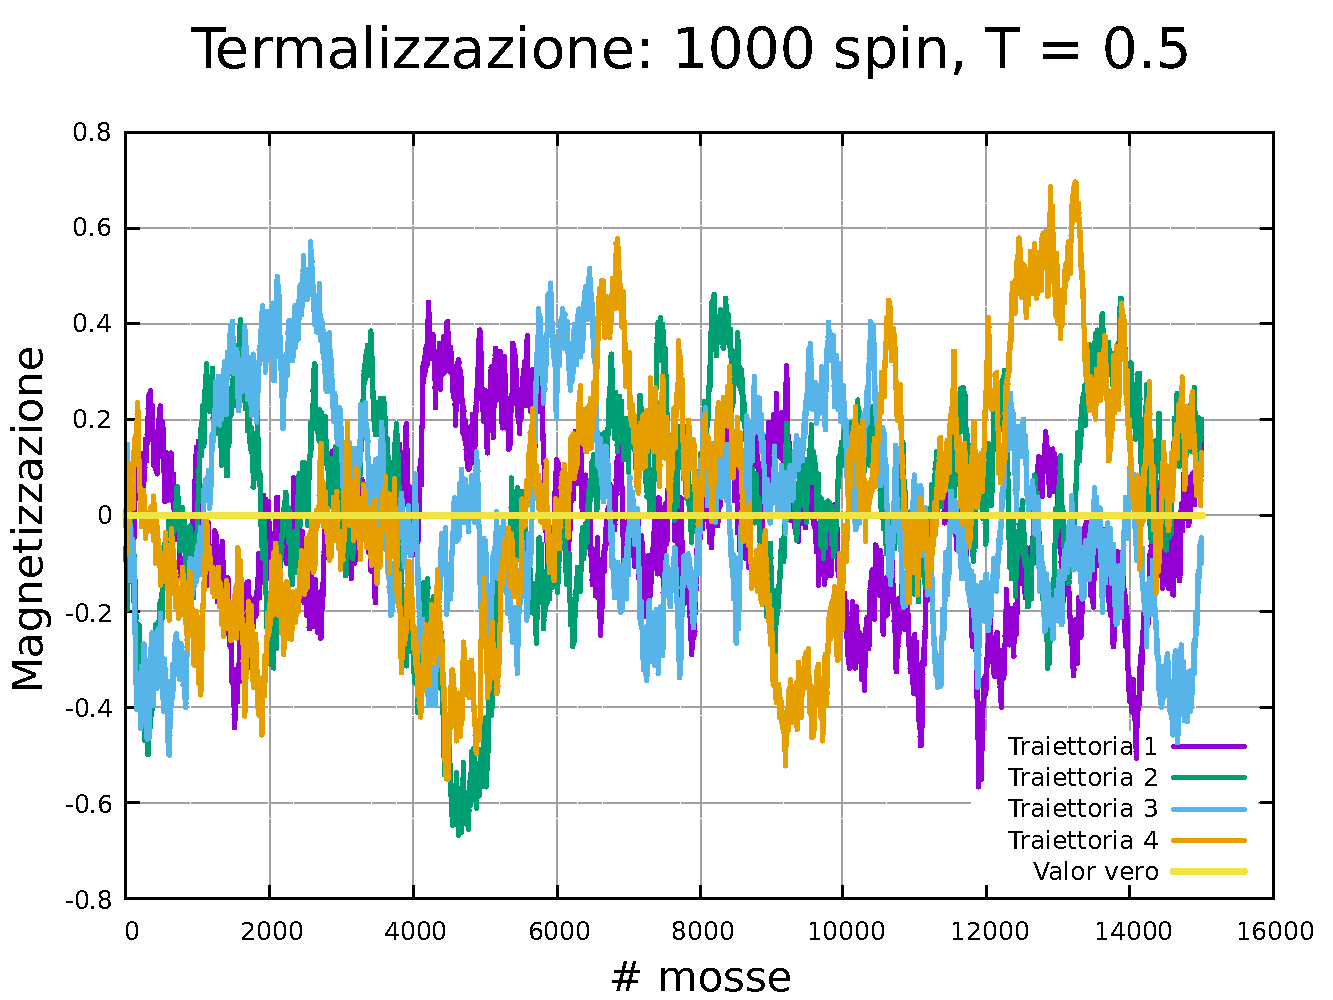
\includegraphics[page=1, width=\textwidth]{Immagini/simIsing1D/magn0.0/term/term_1000_0.5.pdf}
      \caption{$T\,=\,0.5$}
    \end{minipage}\hfill
    \begin{minipage}{0.45\textwidth}  
      \centering
      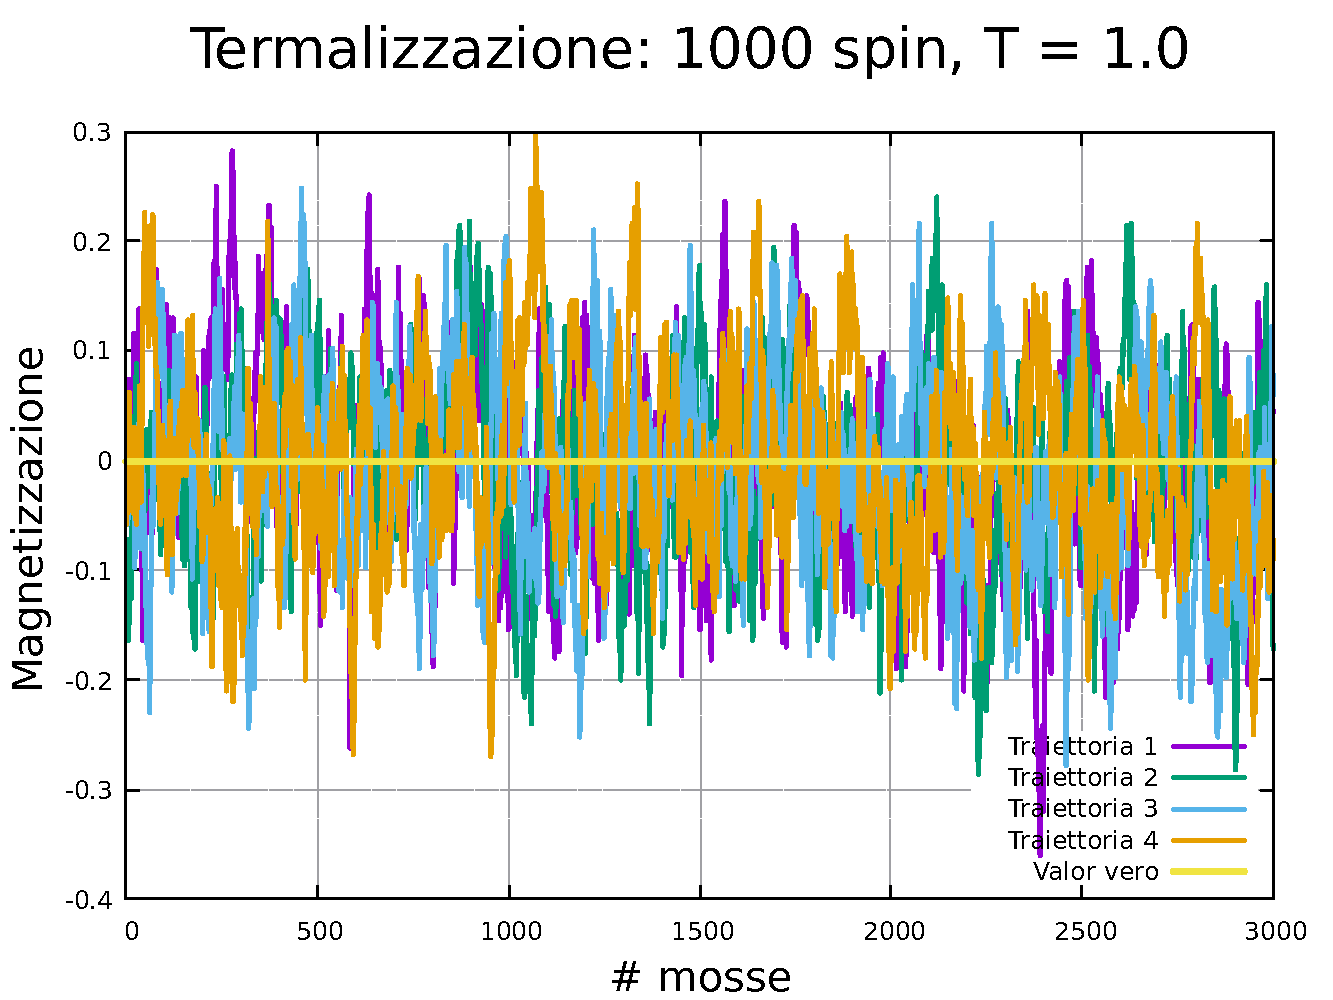
\includegraphics[page=1, width=\textwidth]{Immagini/simIsing1D/magn0.0/term/term_1000_1.0.pdf}
      \caption{$T\,=\,1.0$}
    \end{minipage}
    \vskip\baselineskip 
  
    \begin{minipage}{0.45\textwidth}  
      \centering
      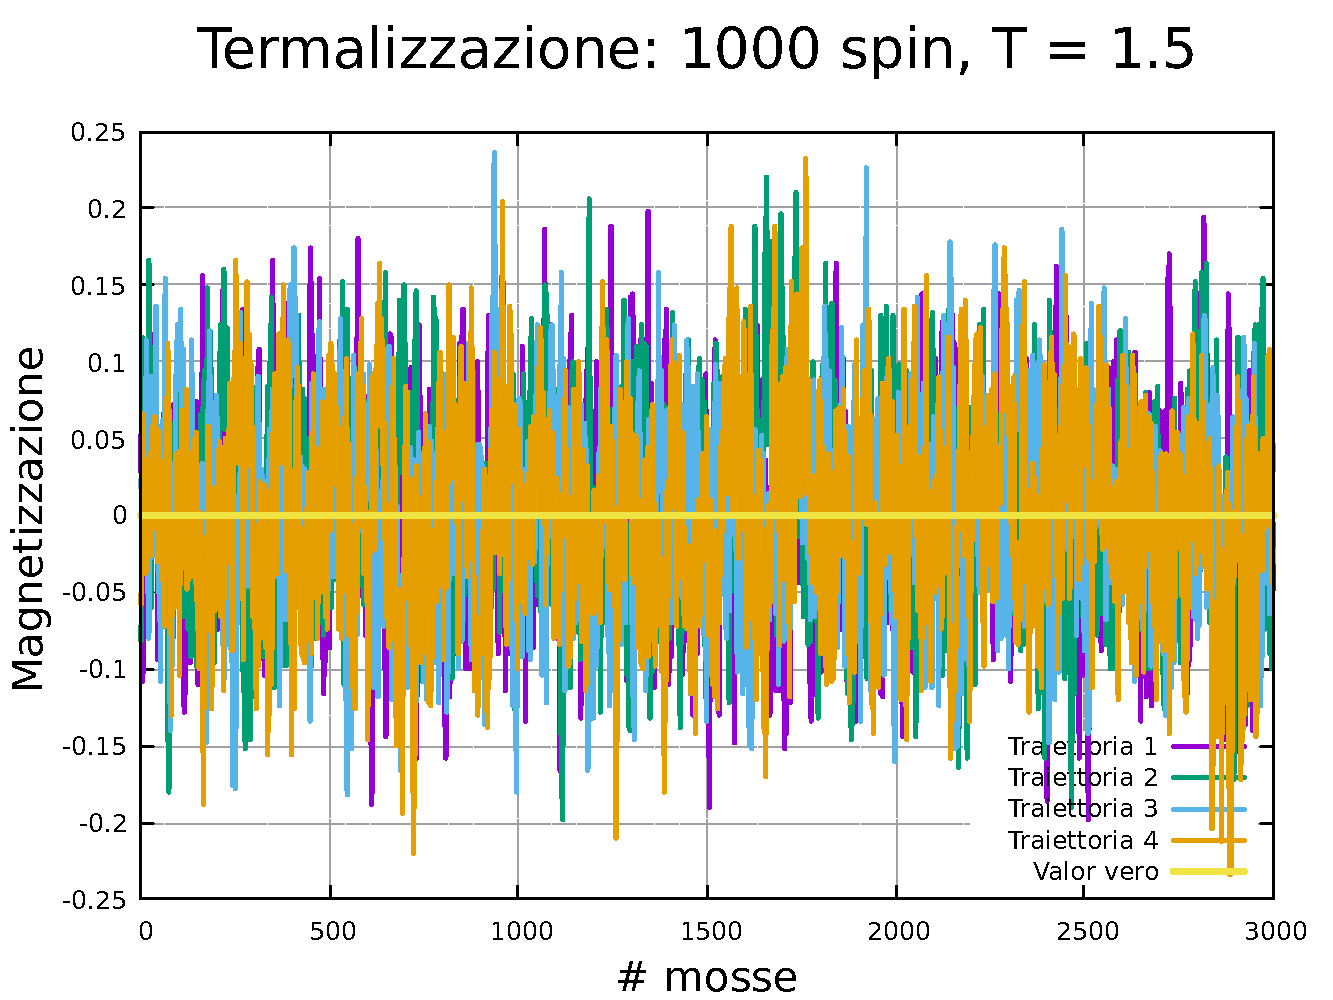
\includegraphics[page=1, width=\textwidth]{Immagini/simIsing1D/magn0.0/term/term_1000_1.5.pdf}
      \caption{$T\,=\,1.5$}
    \end{minipage}\hfill
    \begin{minipage}{0.45\textwidth}  
      \centering
      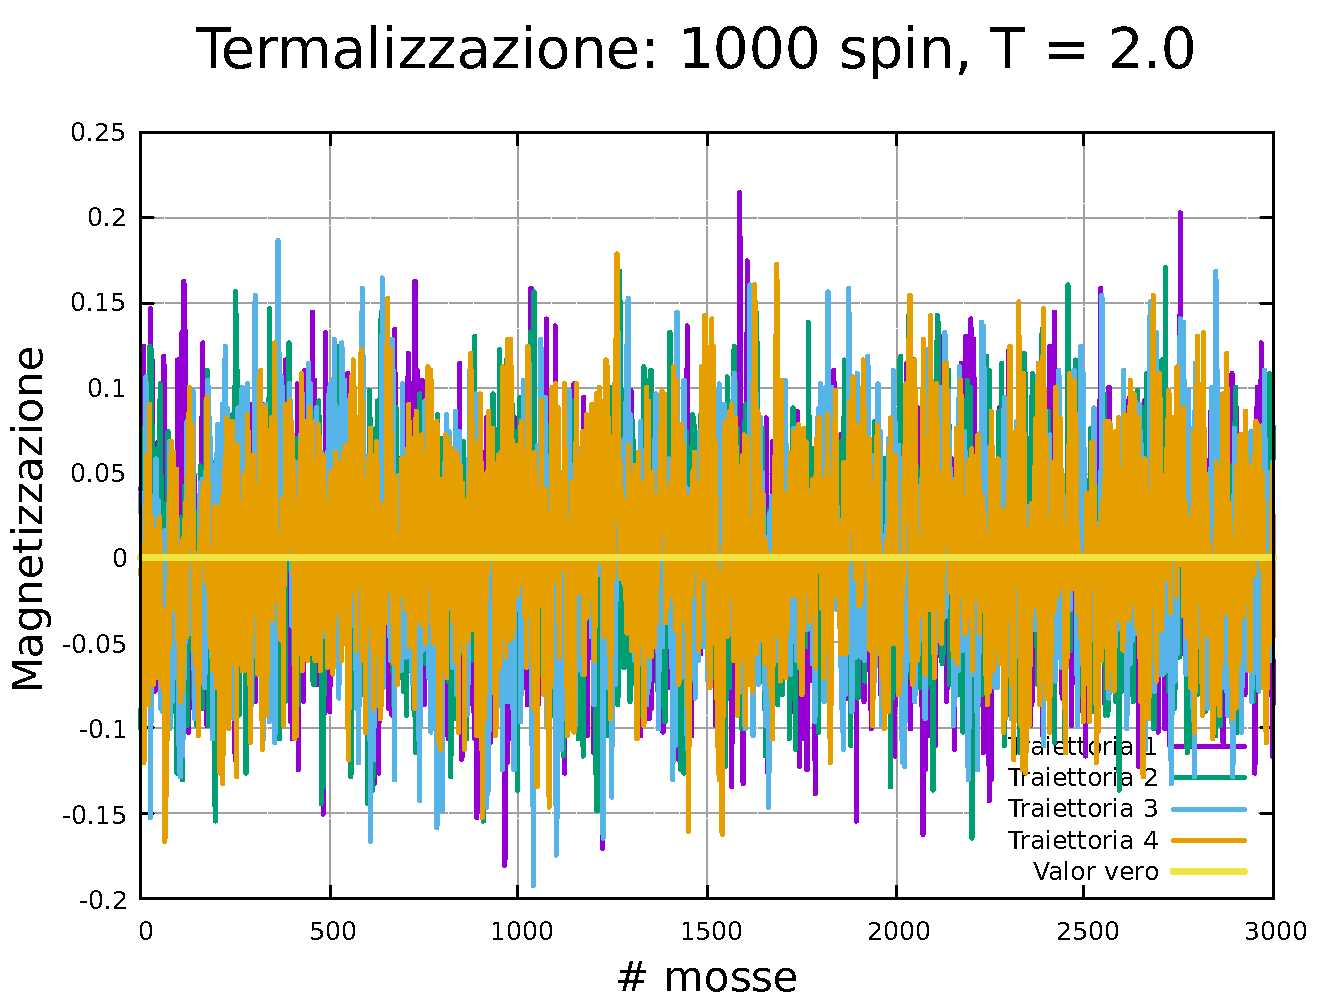
\includegraphics[page=1, width=\textwidth]{Immagini/simIsing1D/magn0.0/term/term_1000_2.0.pdf}
      \caption{$T\,=\,2.0$}
    \end{minipage}
    \caption{Studio della termalizzazione di un modello di Ising 1D costituito da 1000 spin.}
\end{figure}

\vspace*{\fill}

\newpage

\vspace*{\fill}

\begin{figure}[htbp]
    \centering
    \begin{minipage}{0.45\textwidth}  
      \centering
      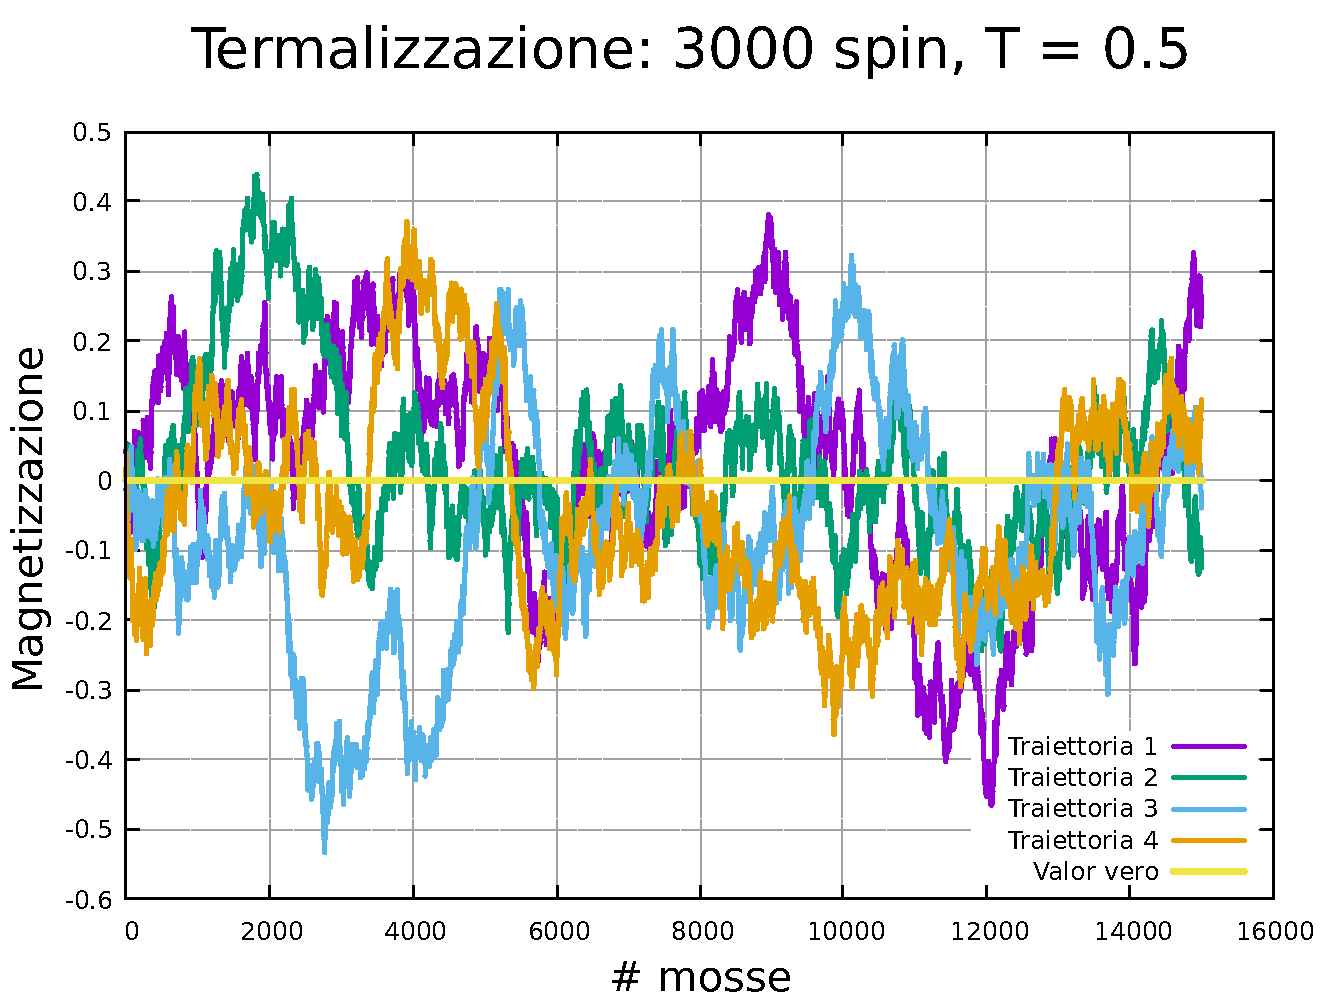
\includegraphics[page=1, width=\textwidth]{Immagini/simIsing1D/magn0.0/term/term_3000_0.5.pdf}
      \caption{$T\,=\,0.5$}
    \end{minipage}\hfill
    \begin{minipage}{0.45\textwidth}  
      \centering
      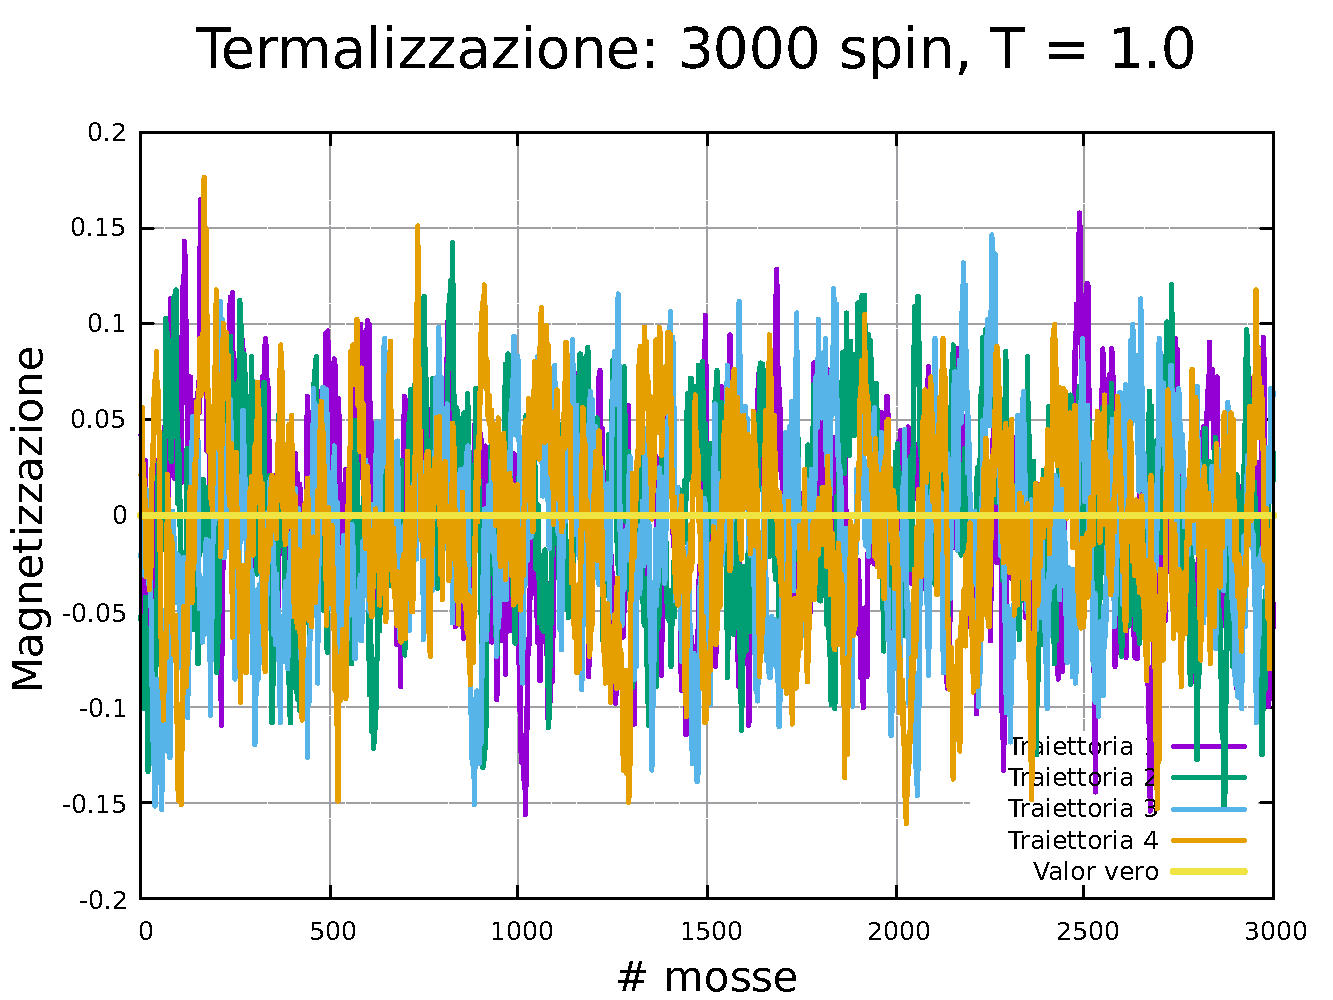
\includegraphics[page=1, width=\textwidth]{Immagini/simIsing1D/magn0.0/term/term_3000_1.0.pdf}
      \caption{$T\,=\,1.0$}
    \end{minipage}
    \vskip\baselineskip 
  
    \begin{minipage}{0.45\textwidth}  
      \centering
      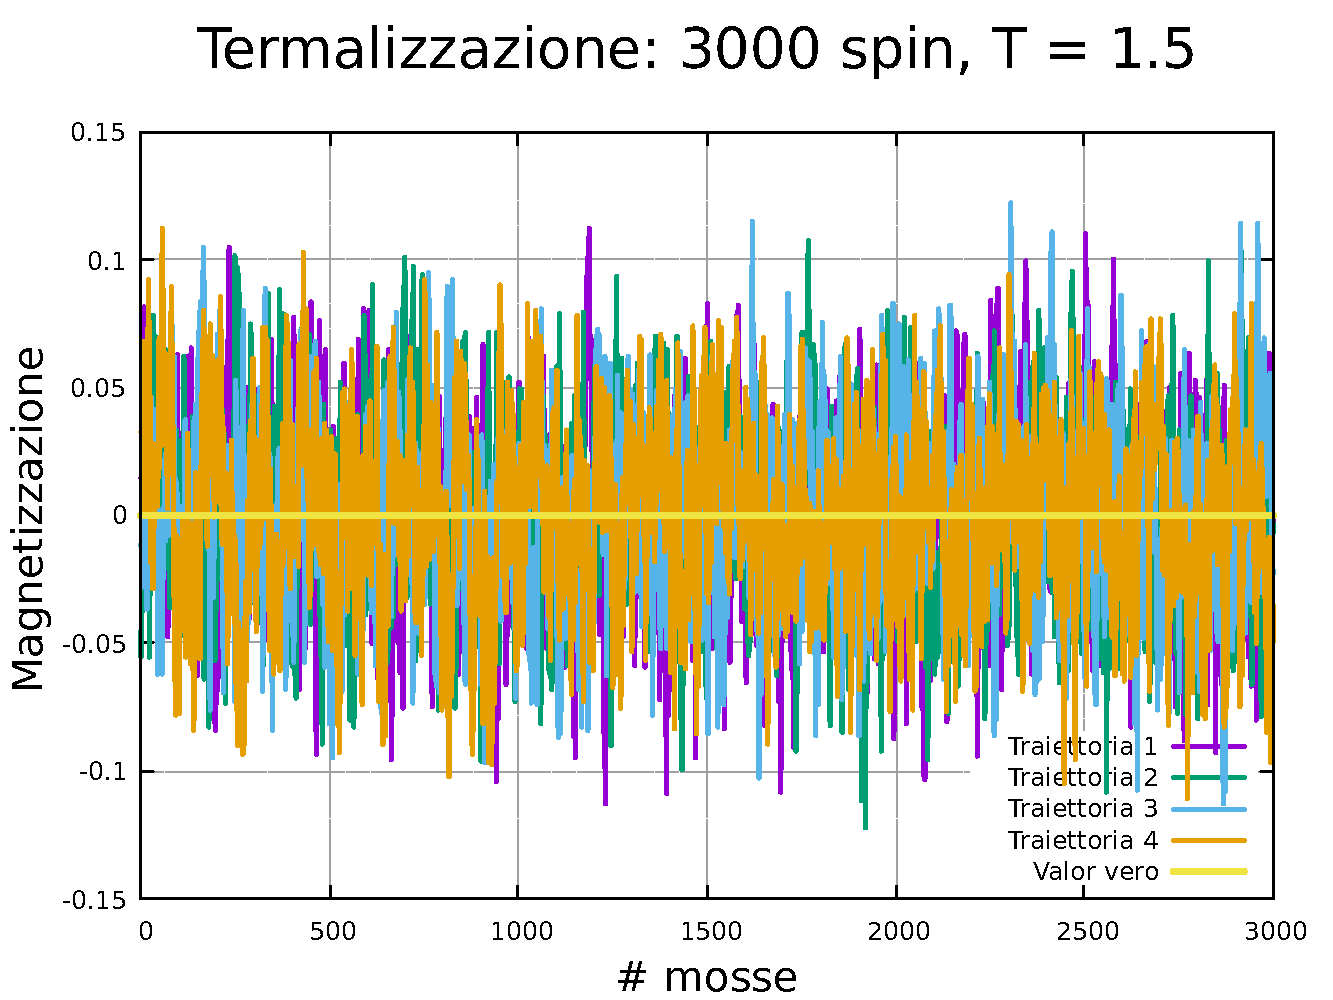
\includegraphics[page=1, width=\textwidth]{Immagini/simIsing1D/magn0.0/term/term_3000_1.5.pdf}
      \caption{$T\,=\,1.5$}
    \end{minipage}\hfill
    \begin{minipage}{0.45\textwidth}  
      \centering
      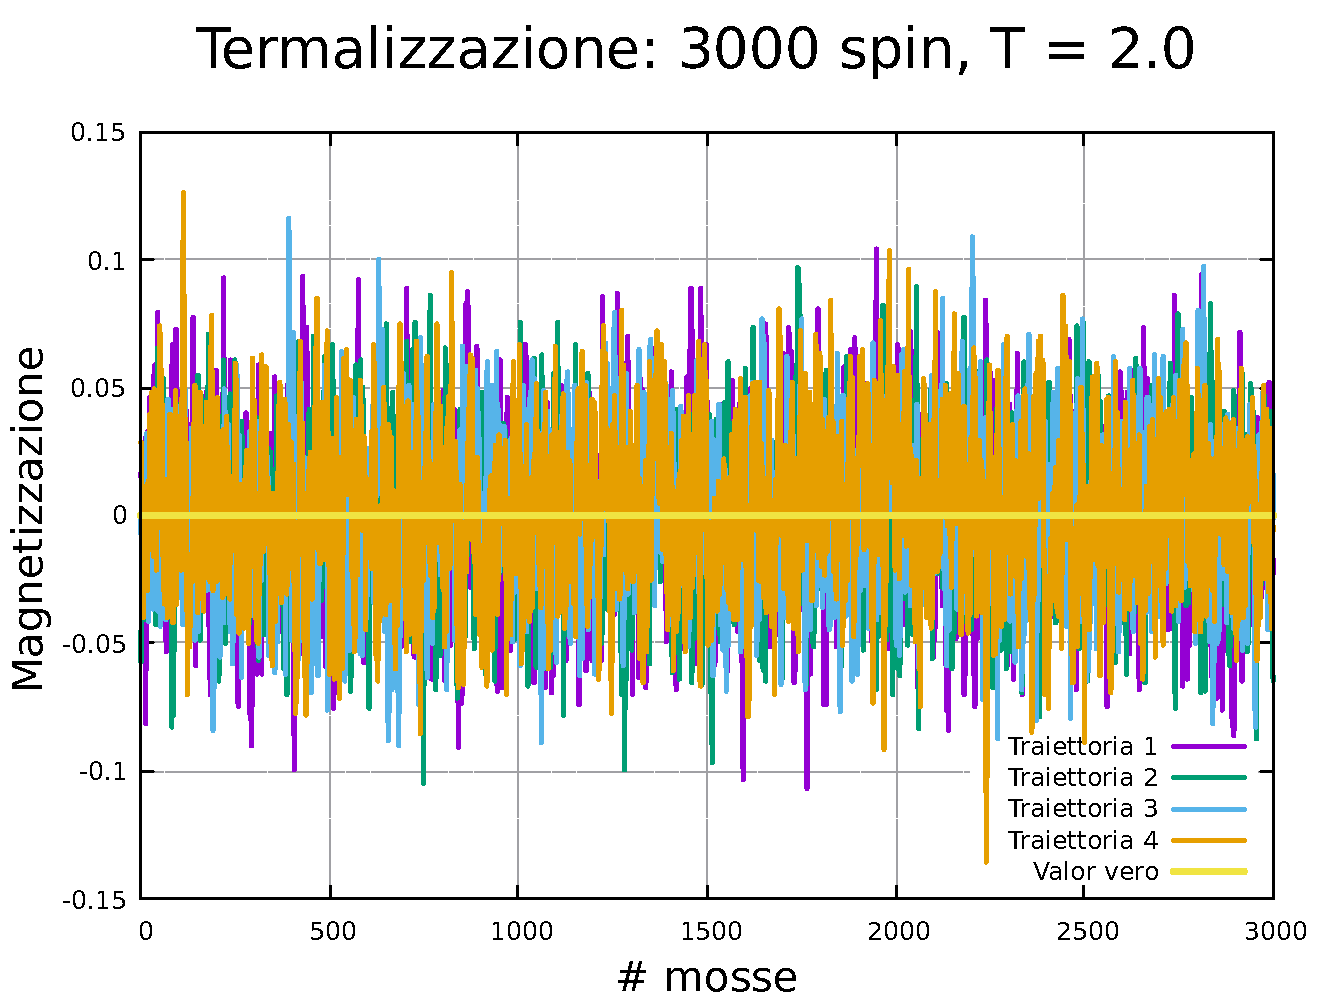
\includegraphics[page=1, width=\textwidth]{Immagini/simIsing1D/magn0.0/term/term_3000_2.0.pdf}
      \caption{$T\,=\,2.0$}
    \end{minipage}
    \caption{Studio della termalizzazione di un modello di Ising 1D costituito da 3000 spin.}
\end{figure}

\vspace*{\fill}

\newpage

\vspace*{\fill}

\begin{figure}[htbp]
    \centering
    \begin{minipage}{0.45\textwidth}  
      \centering
      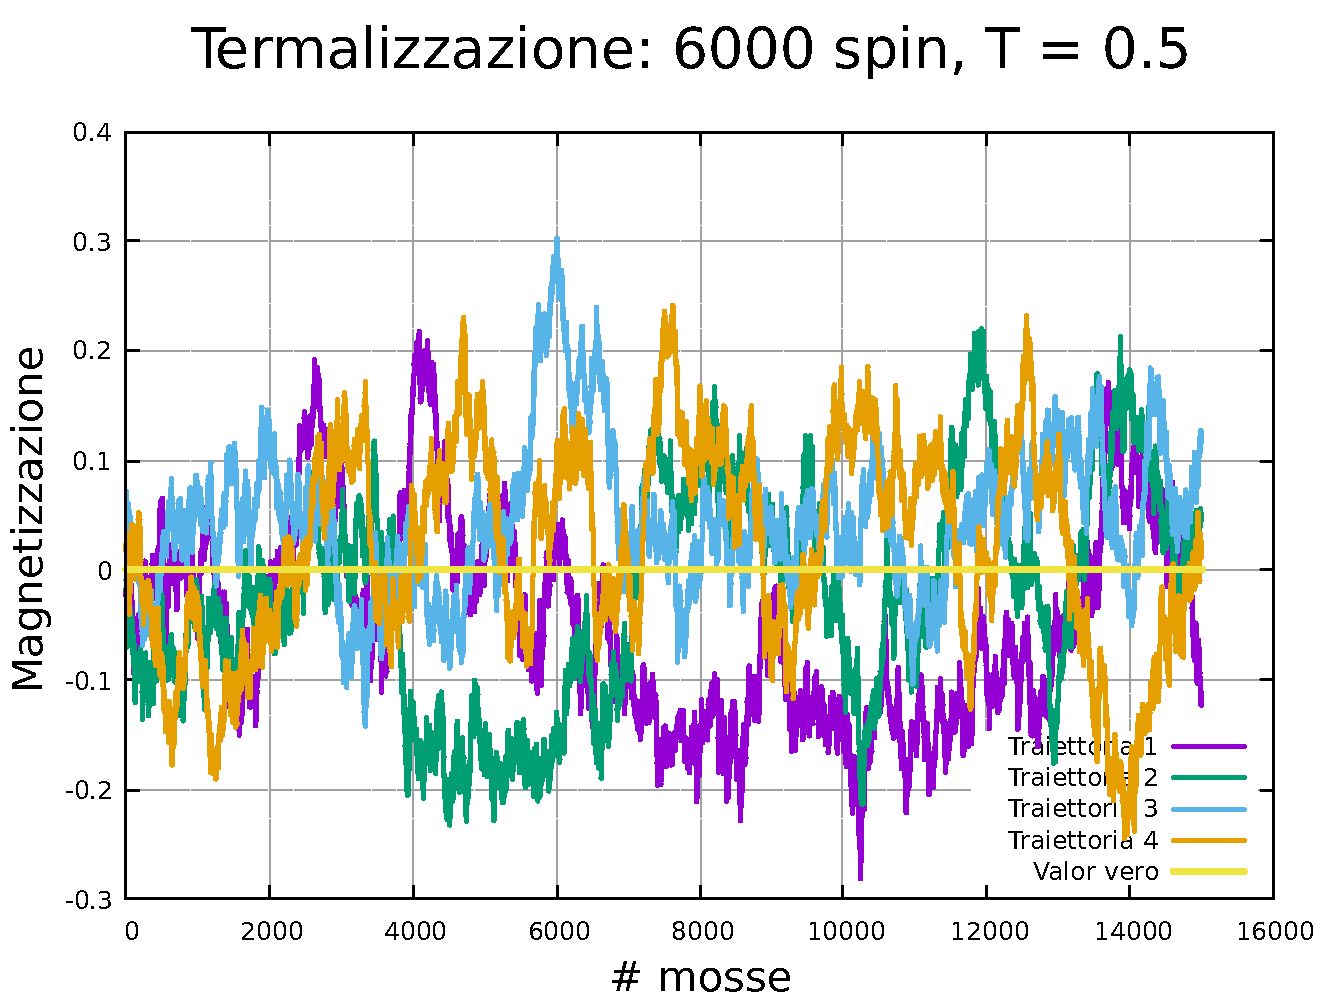
\includegraphics[page=1, width=\textwidth]{Immagini/simIsing1D/magn0.0/term/term_6000_0.5.pdf}
      \caption{$T\,=\,0.5$}
    \end{minipage}\hfill
    \begin{minipage}{0.45\textwidth}  
      \centering
      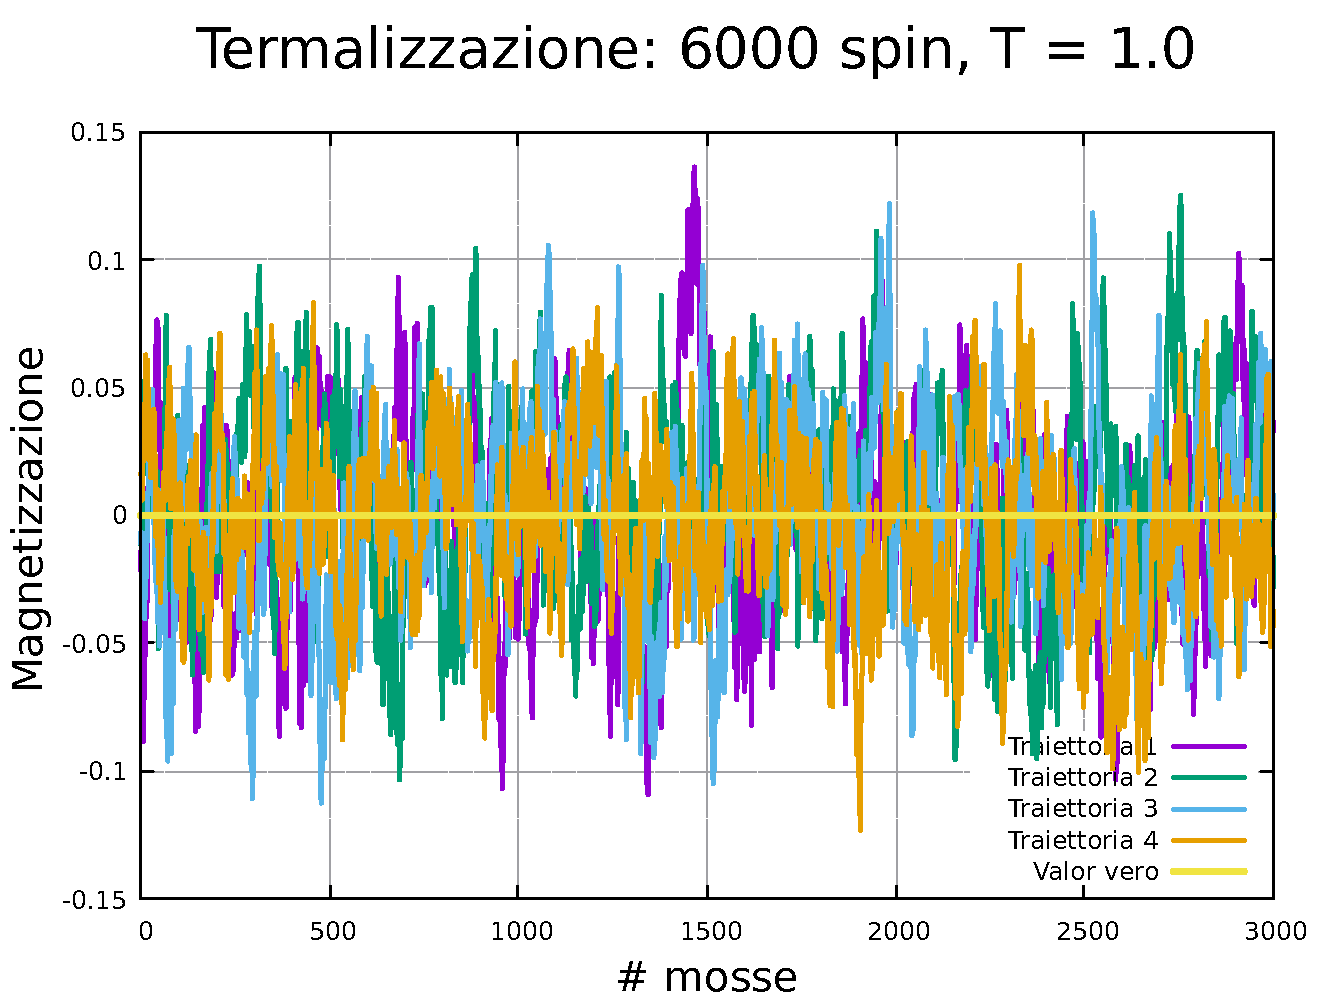
\includegraphics[page=1, width=\textwidth]{Immagini/simIsing1D/magn0.0/term/term_6000_1.0.pdf}
      \caption{$T\,=\,1.0$}
    \end{minipage}
    \vskip\baselineskip 
  
    \begin{minipage}{0.45\textwidth}  
      \centering
      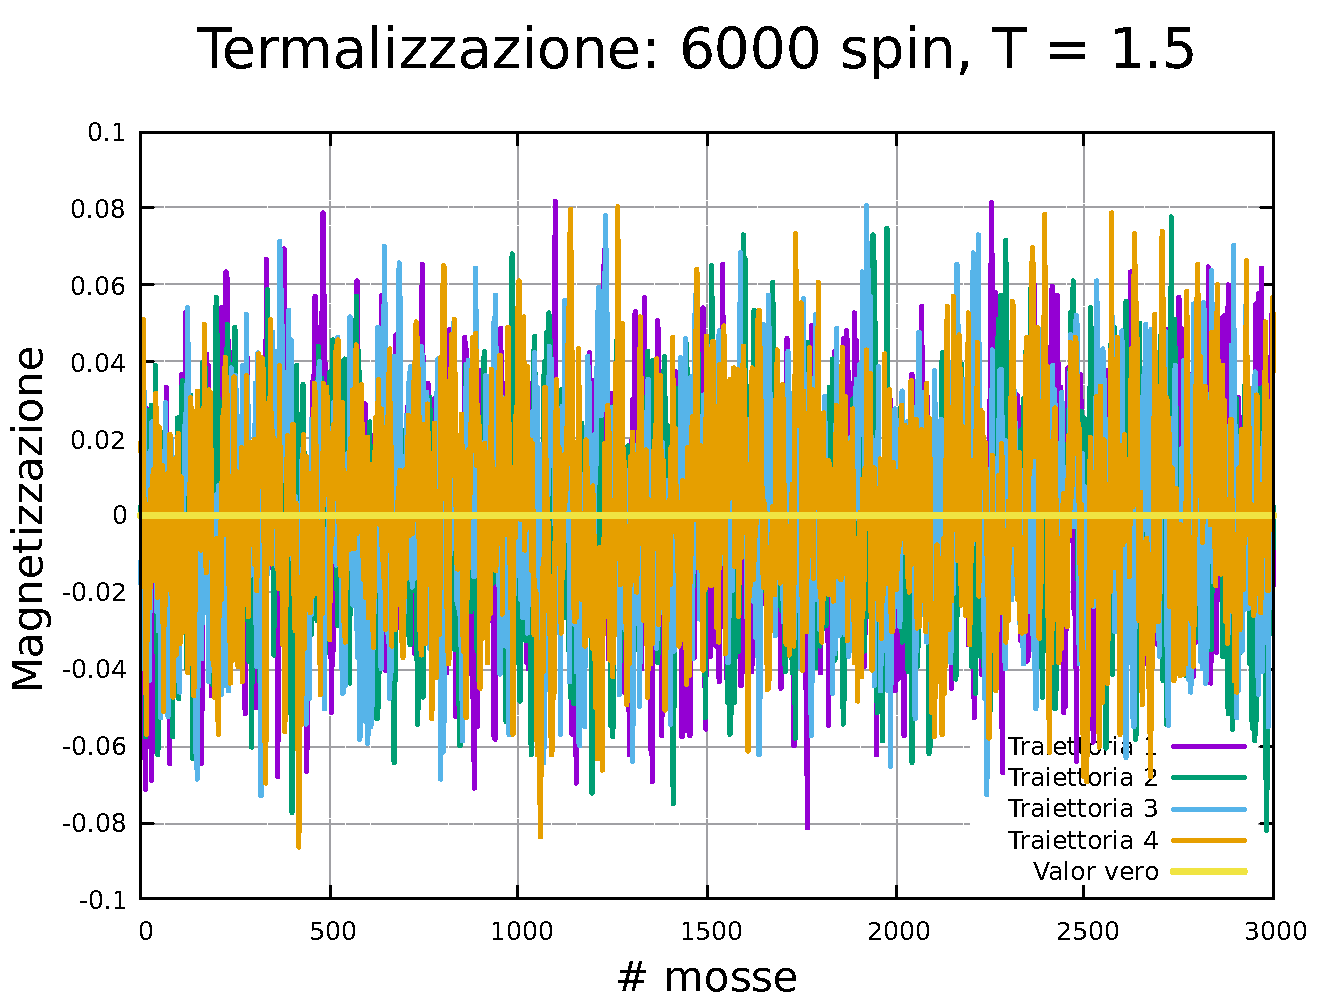
\includegraphics[page=1, width=\textwidth]{Immagini/simIsing1D/magn0.0/term/term_6000_1.5.pdf}
      \caption{$T\,=\,1.5$}
    \end{minipage}\hfill
    \begin{minipage}{0.45\textwidth}  
      \centering
      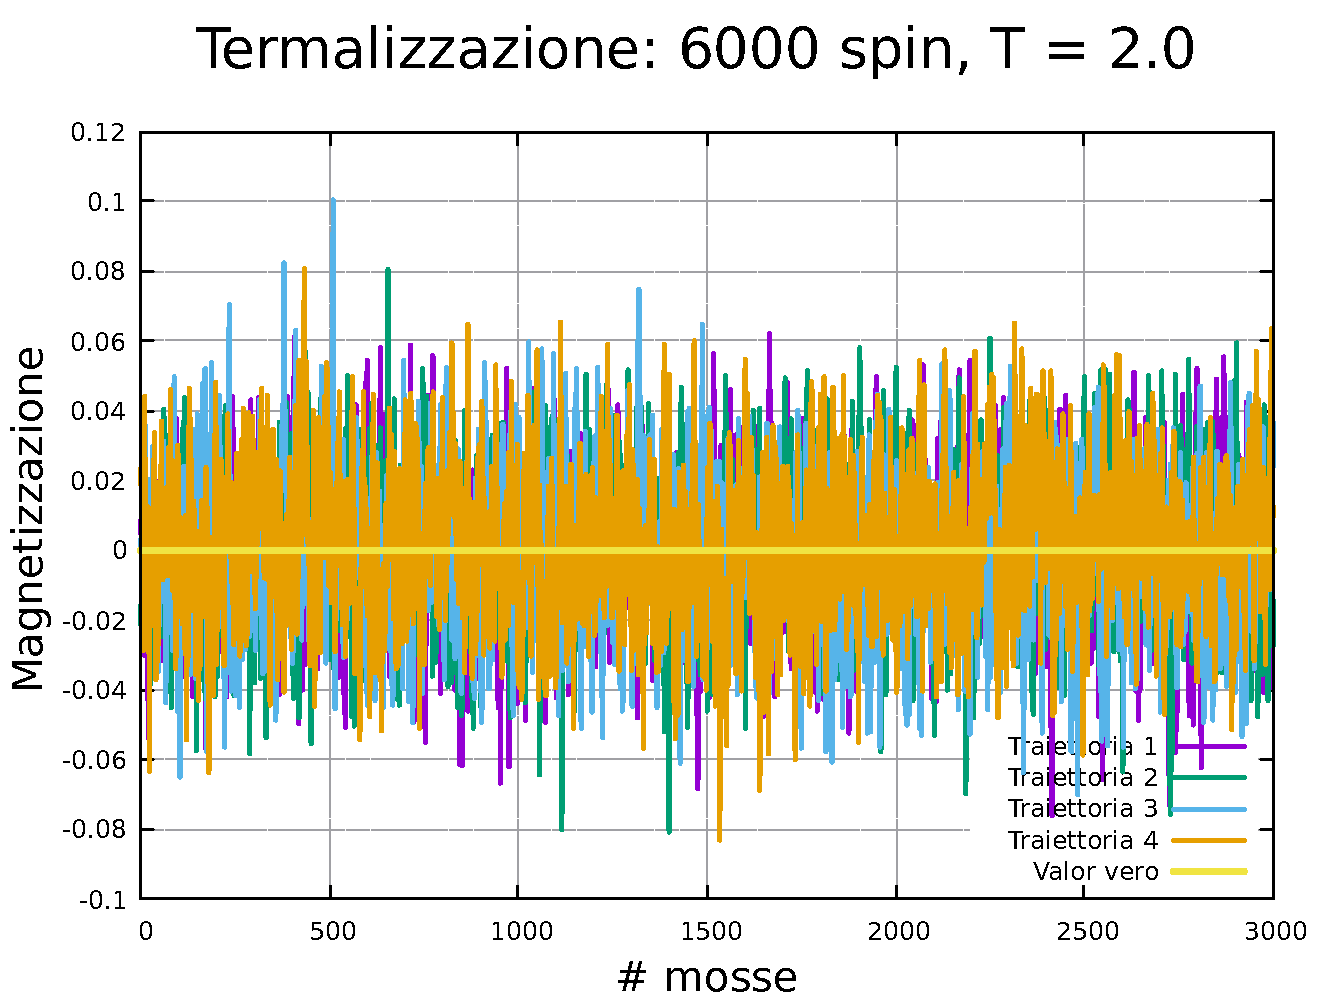
\includegraphics[page=1, width=\textwidth]{Immagini/simIsing1D/magn0.0/term/term_6000_2.0.pdf}
      \caption{$T\,=\,2.0$}
    \end{minipage}
    \caption{Studio della termalizzazione di un modello di Ising 1D costituito da 6000 spin.}
\end{figure}

\vspace*{\fill}

\newpage

\vspace*{\fill}

\begin{figure}[htbp]
    \centering
    \begin{minipage}{0.45\textwidth}  
      \centering
      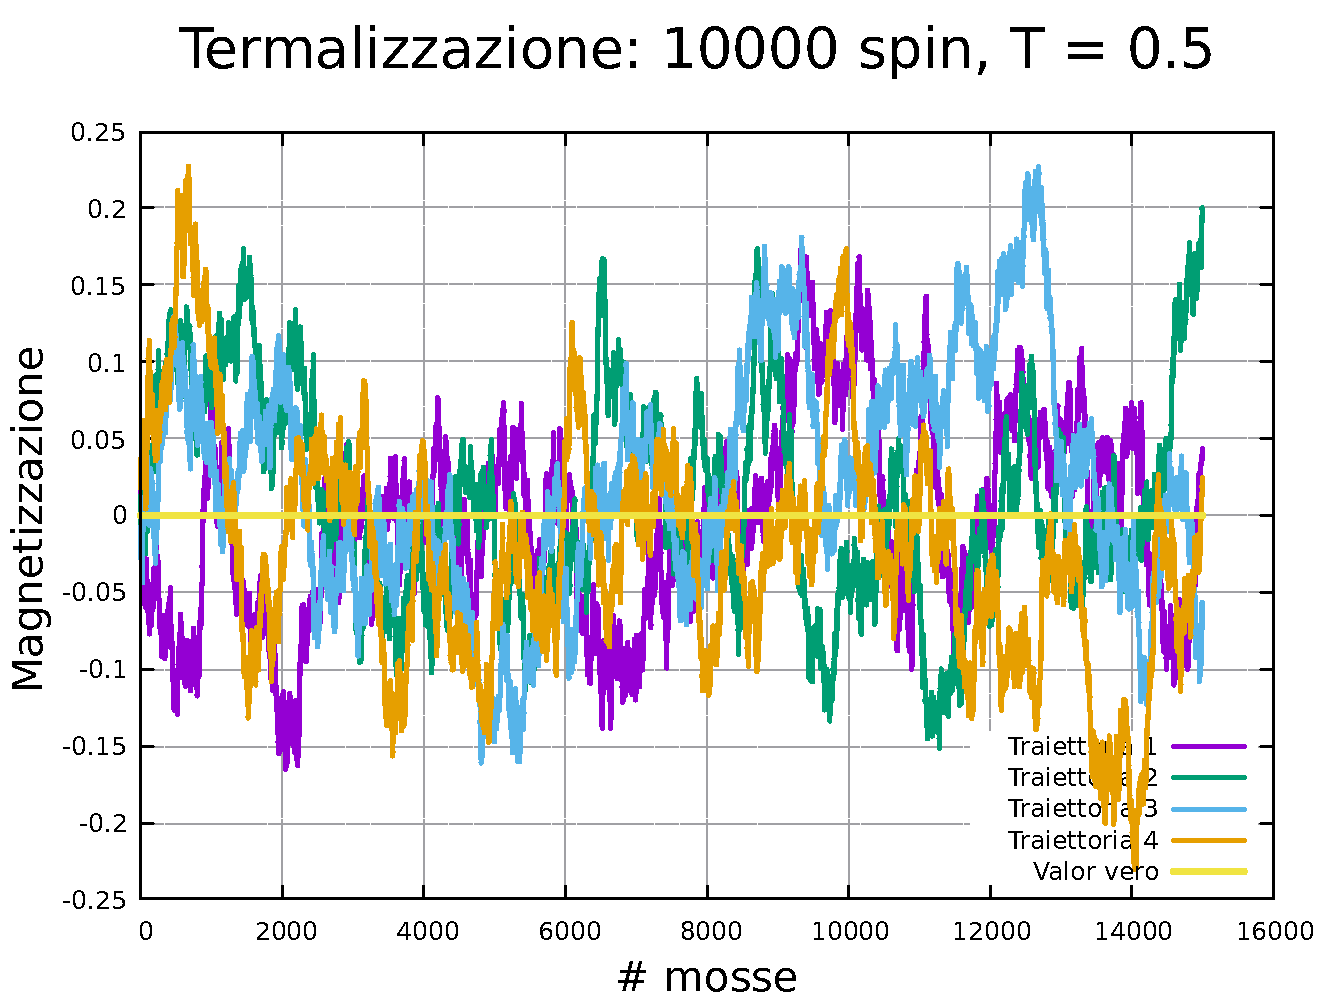
\includegraphics[page=1, width=\textwidth]{Immagini/simIsing1D/magn0.0/term/term_10000_0.5.pdf}
      \caption{$T\,=\,0.5$}
    \end{minipage}\hfill
    \begin{minipage}{0.45\textwidth}  
      \centering
      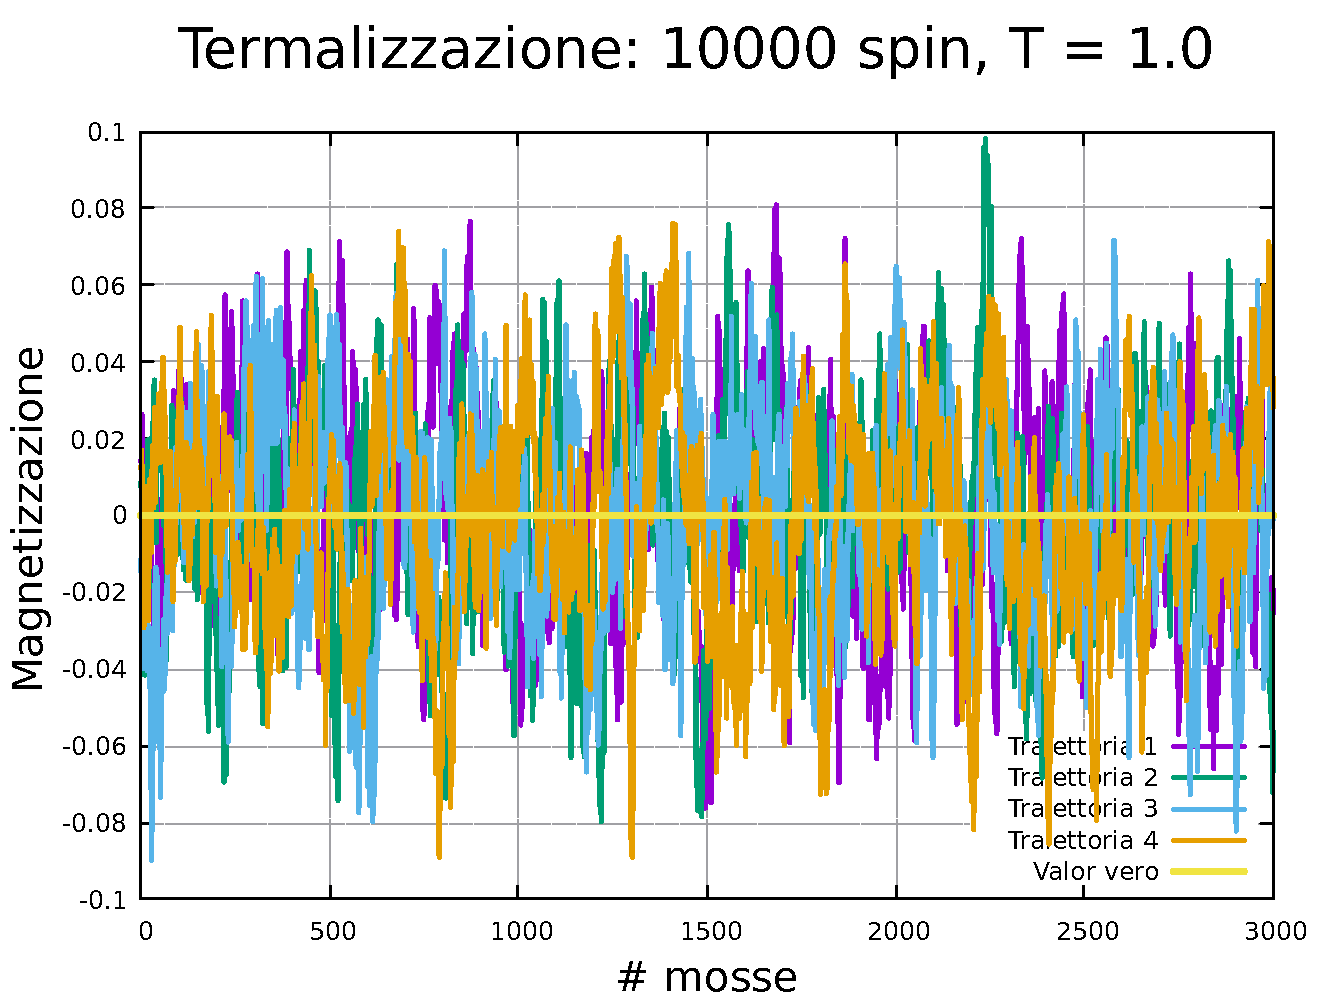
\includegraphics[page=1, width=\textwidth]{Immagini/simIsing1D/magn0.0/term/term_10000_1.0.pdf}
      \caption{$T\,=\,1.0$}
    \end{minipage}
    \vskip\baselineskip 
  
    \begin{minipage}{0.45\textwidth}  
      \centering
      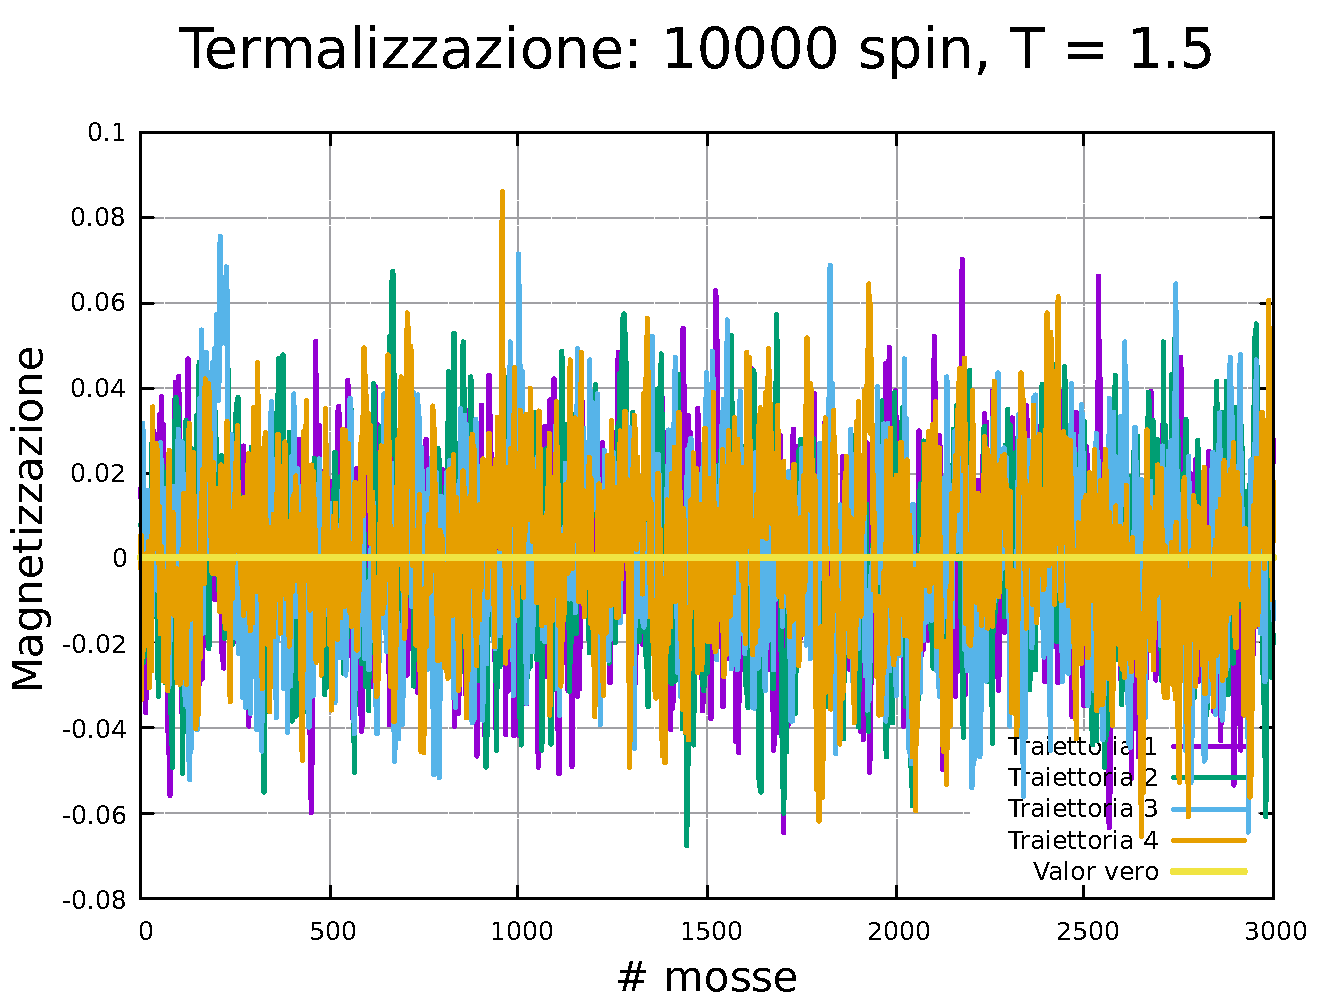
\includegraphics[page=1, width=\textwidth]{Immagini/simIsing1D/magn0.0/term/term_10000_1.5.pdf}
      \caption{$T\,=\,1.5$}
    \end{minipage}\hfill
    \begin{minipage}{0.45\textwidth}  
      \centering
      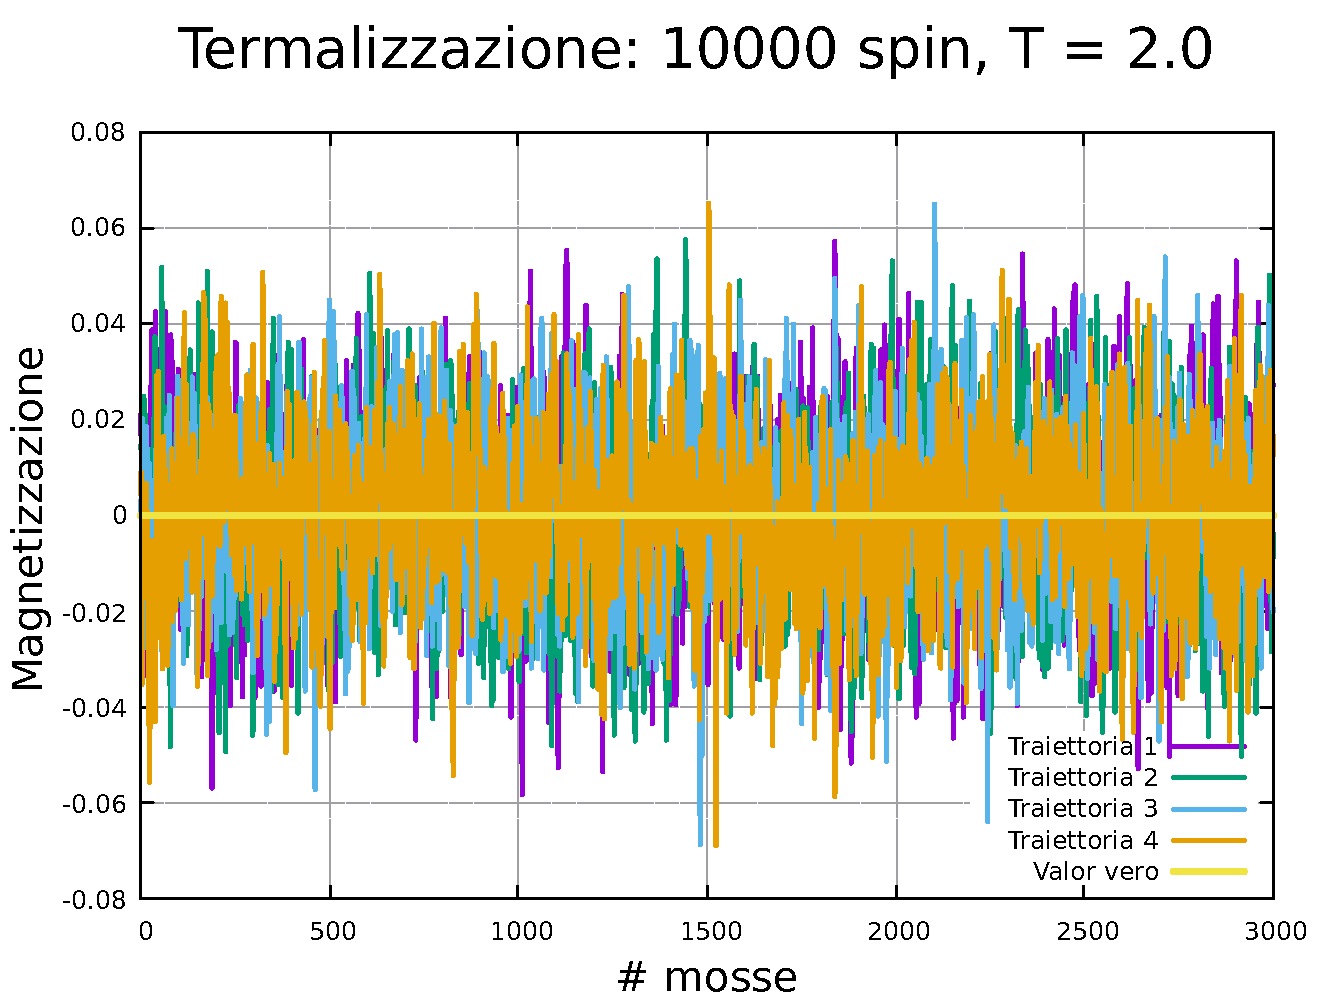
\includegraphics[page=1, width=\textwidth]{Immagini/simIsing1D/magn0.0/term/term_10000_2.0.pdf}
      \caption{$T\,=\,2.0$}
    \end{minipage}
    \caption{Studio della termalizzazione di un modello di Ising 1D costituito da 10000 spin.}
\end{figure}

\vspace*{\fill}

\newpage



\subsection{Auto-correlazione}

\vspace*{\fill}

\begin{figure}[htbp]
    \centering
    \begin{minipage}{0.45\textwidth}  
      \centering
      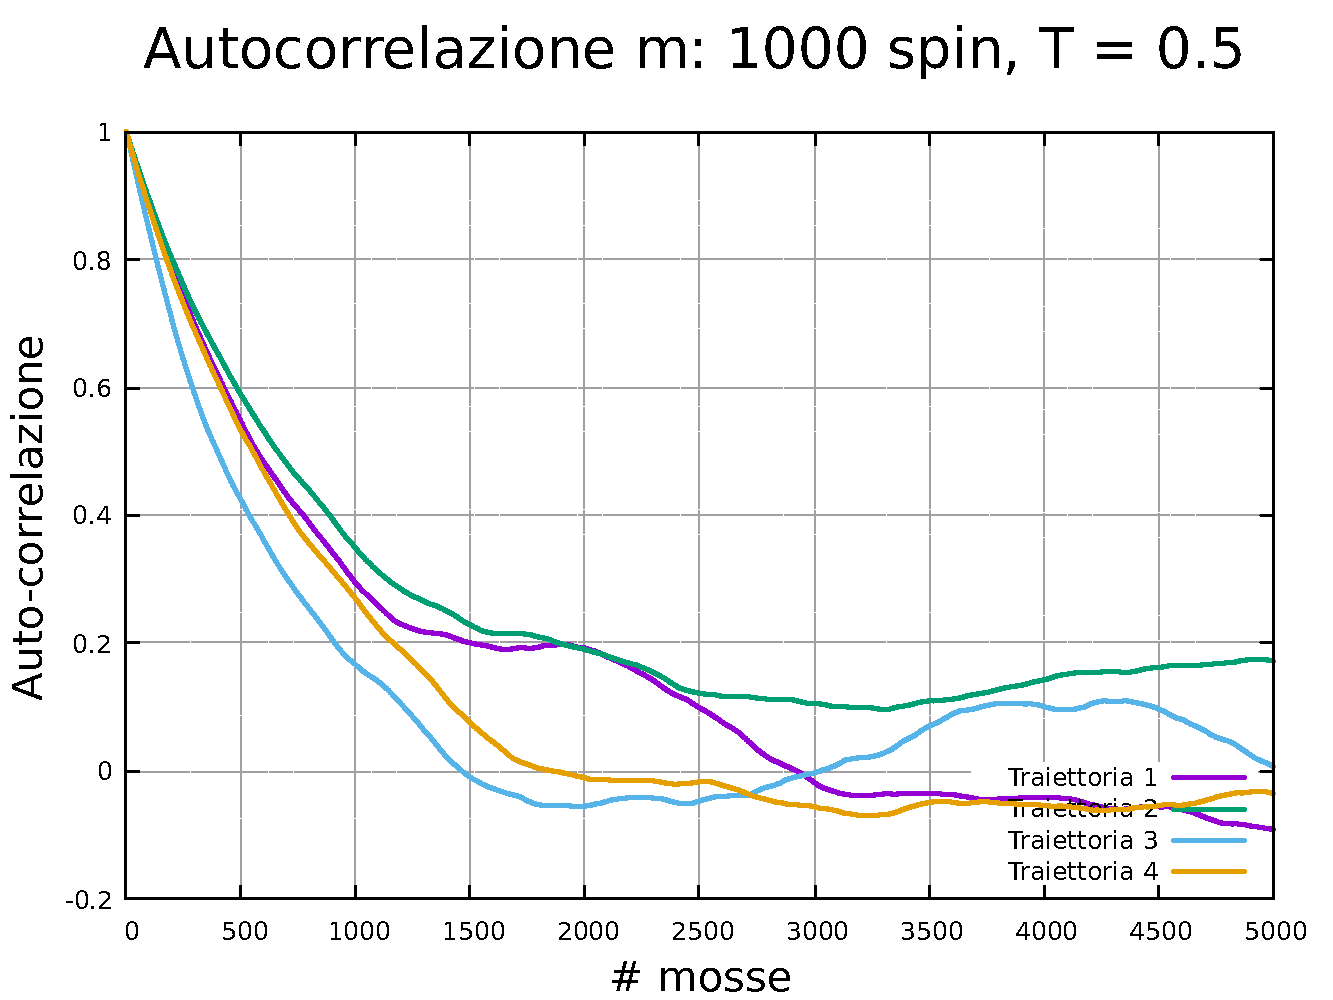
\includegraphics[page=1, width=\textwidth]{Immagini/simIsing1D/magn0.0/tcorr/auto_1000_0.5.pdf}
      \caption{$T\,=\,0.5$}
    \end{minipage}\hfill
    \begin{minipage}{0.45\textwidth}  
      \centering
      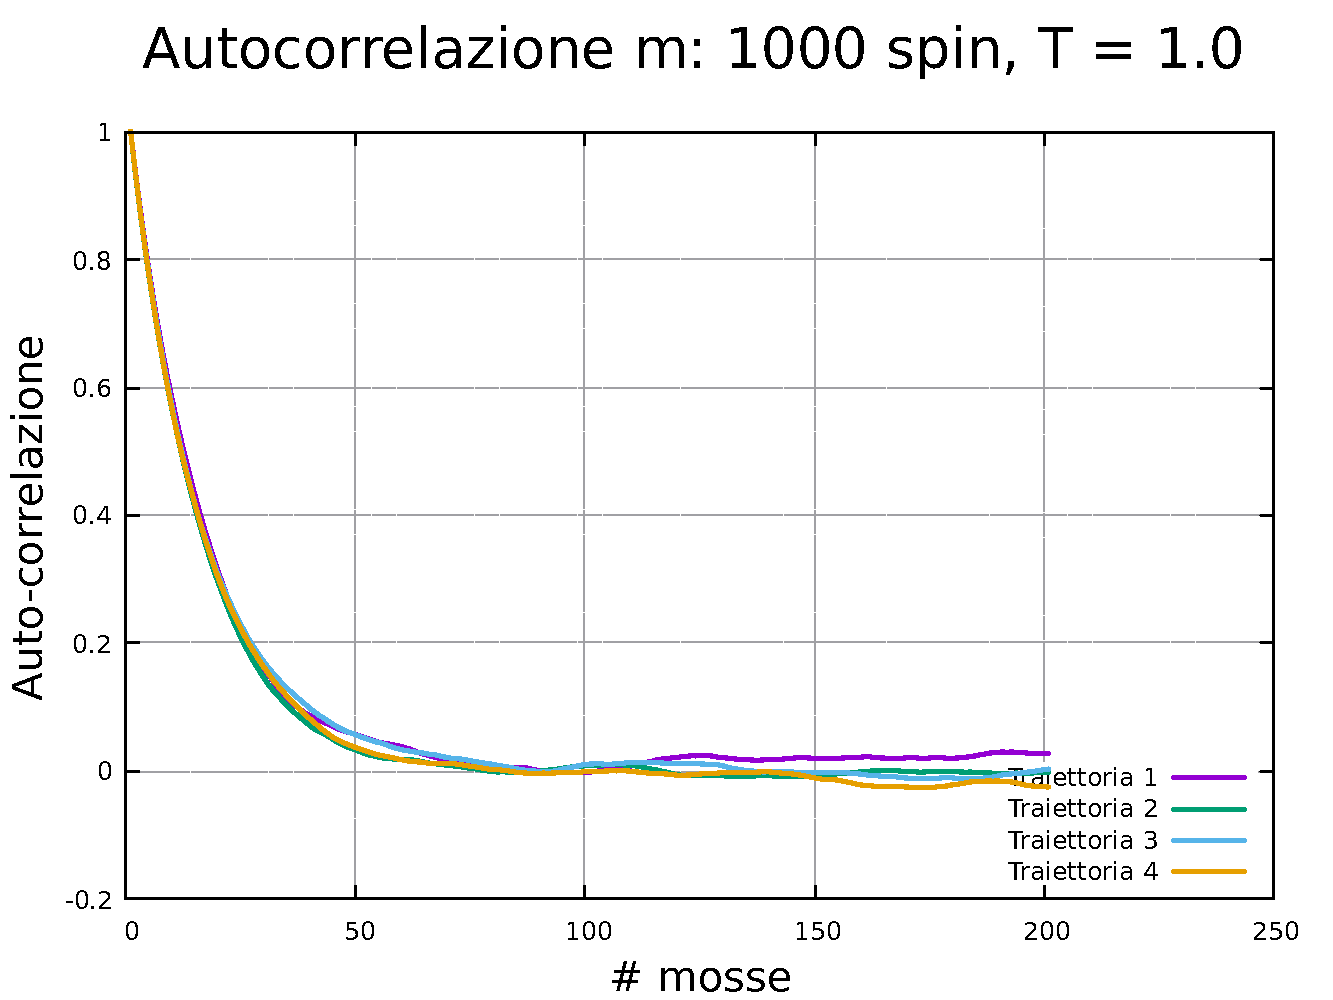
\includegraphics[page=1, width=\textwidth]{Immagini/simIsing1D/magn0.0/tcorr/auto_1000_1.0.pdf}
      \caption{$T\,=\,1.0$}
    \end{minipage}
    \vskip\baselineskip 
  
    \begin{minipage}{0.45\textwidth}  
      \centering
      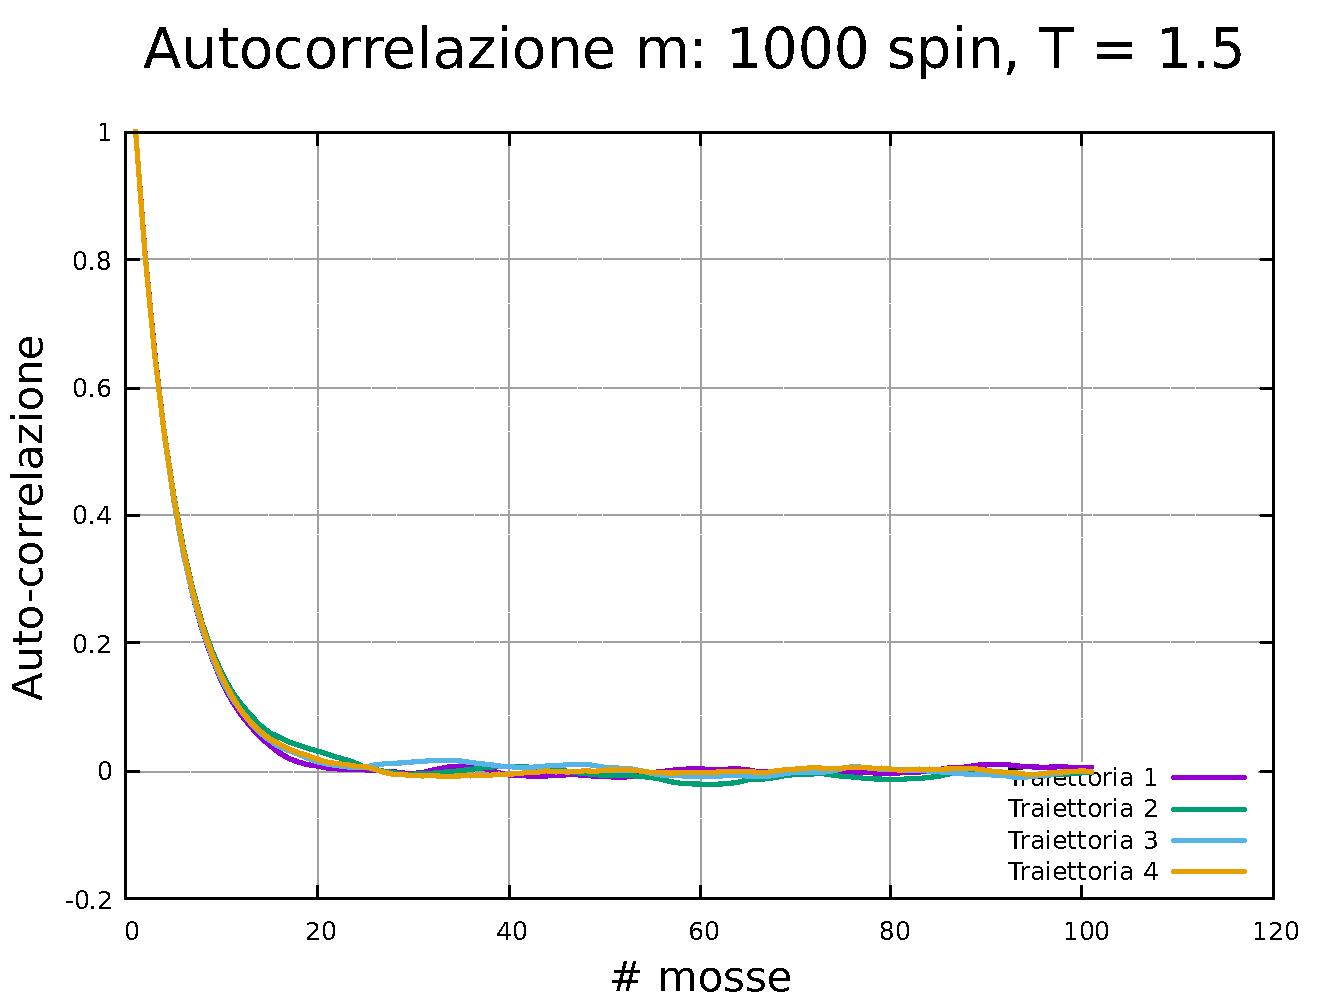
\includegraphics[page=1, width=\textwidth]{Immagini/simIsing1D/magn0.0/tcorr/auto_1000_1.5.pdf}
      \caption{$T\,=\,1.5$}
    \end{minipage}\hfill
    \begin{minipage}{0.45\textwidth}  
      \centering
      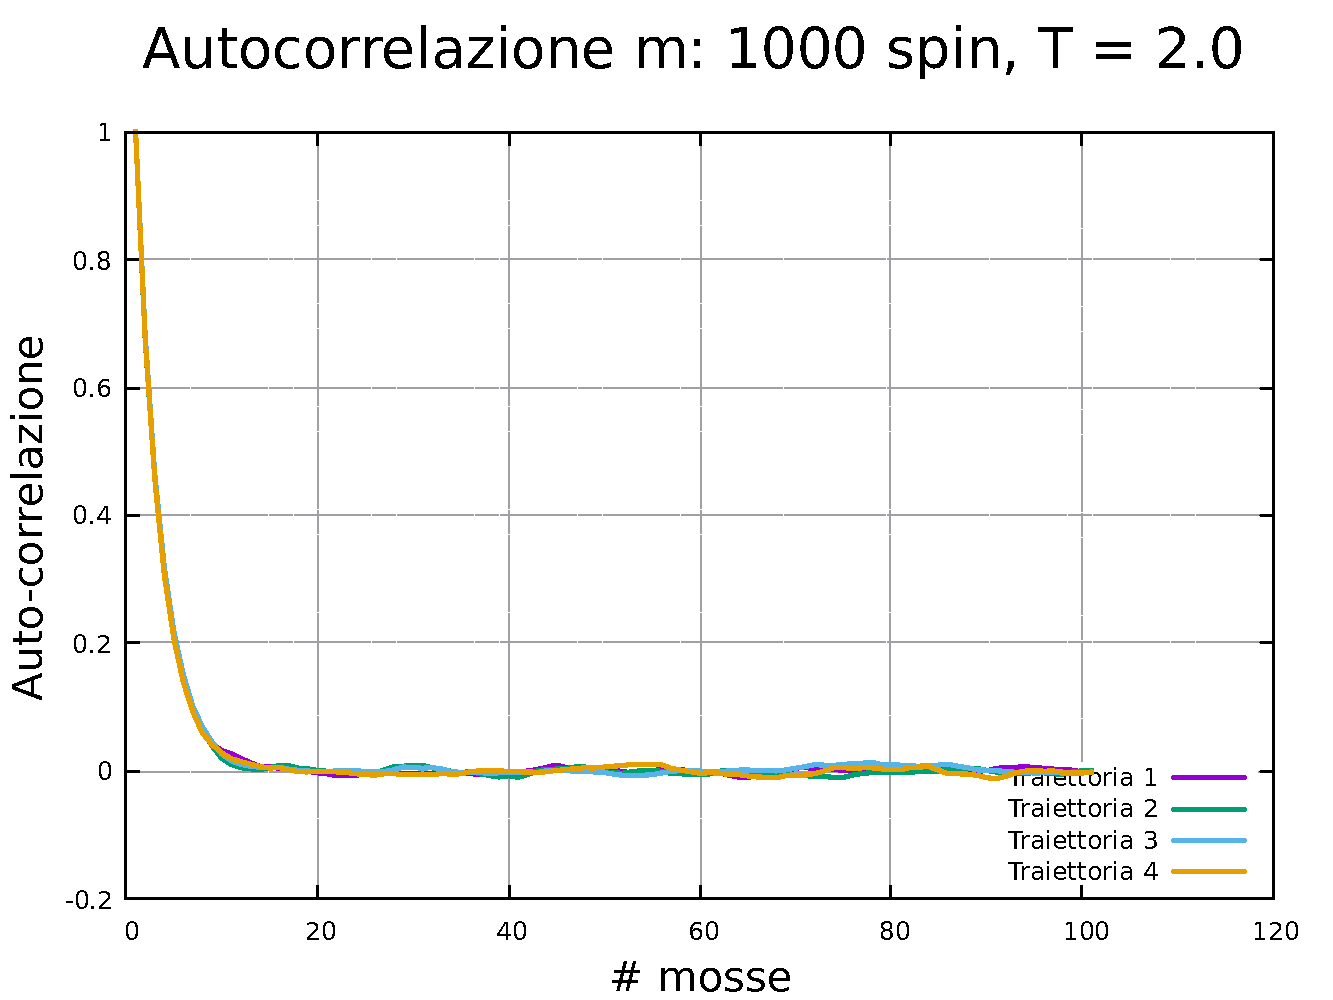
\includegraphics[page=1, width=\textwidth]{Immagini/simIsing1D/magn0.0/tcorr/auto_1000_2.0.pdf}
      \caption{$T\,=\,2.0$}
    \end{minipage}
    \caption{Studio dell'auto-correlazione per un modello di Ising 1D costituito da 1000 spin.}
\end{figure}

\vspace*{\fill}

\newpage

\vspace*{\fill}

\begin{figure}[htbp]
    \centering
    \begin{minipage}{0.45\textwidth}  
      \centering
      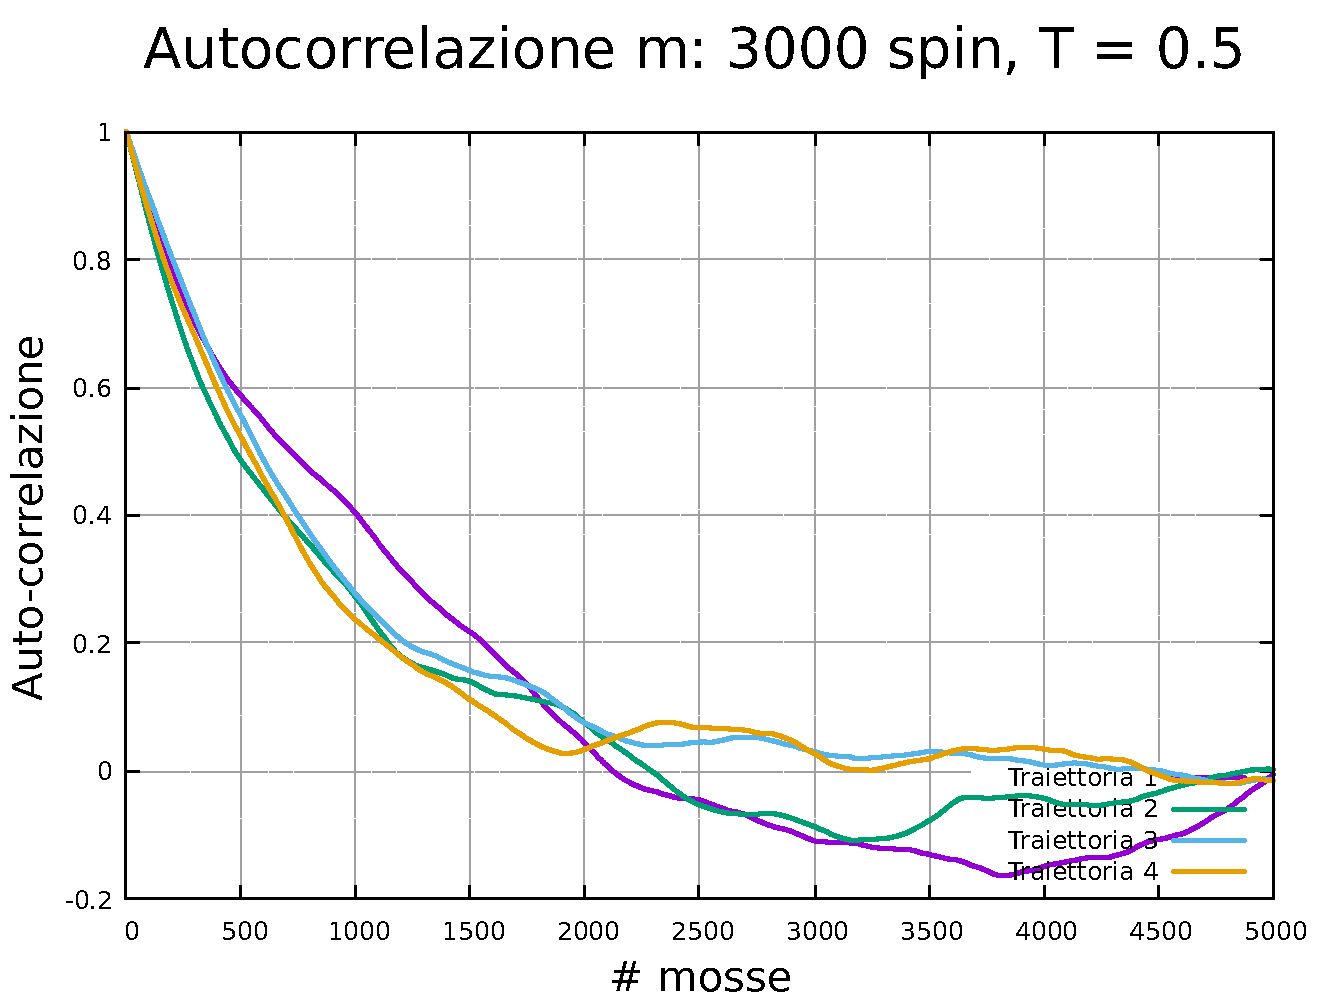
\includegraphics[page=1, width=\textwidth]{Immagini/simIsing1D/magn0.0/tcorr/auto_3000_0.5.pdf}
      \caption{$T\,=\,0.5$}
    \end{minipage}\hfill
    \begin{minipage}{0.45\textwidth}  
      \centering
      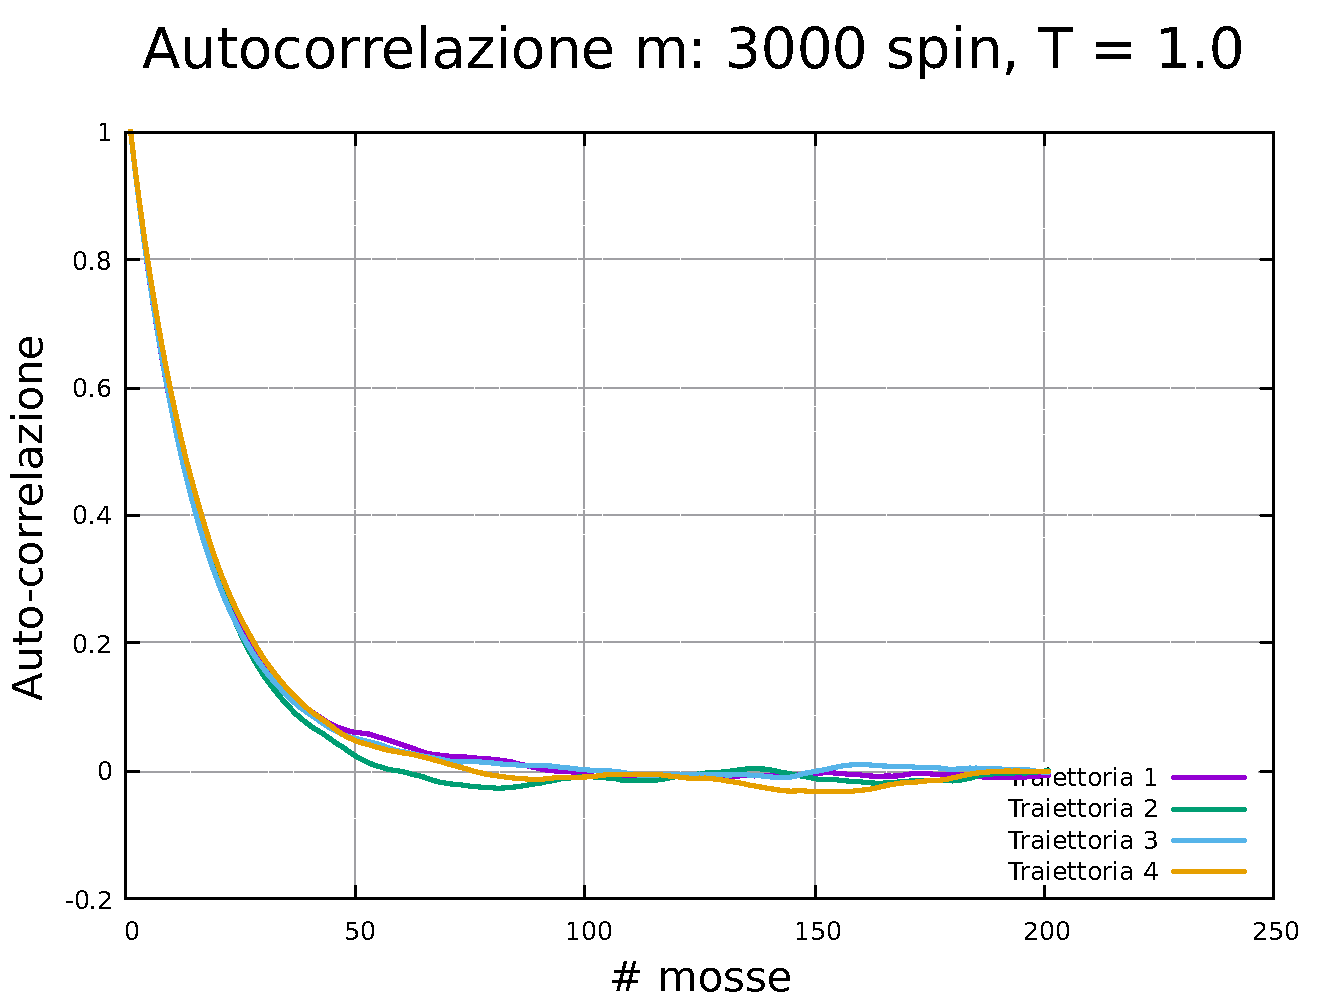
\includegraphics[page=1, width=\textwidth]{Immagini/simIsing1D/magn0.0/tcorr/auto_3000_1.0.pdf}
      \caption{$T\,=\,1.0$}
    \end{minipage}
    \vskip\baselineskip 
  
    \begin{minipage}{0.45\textwidth}  
      \centering
      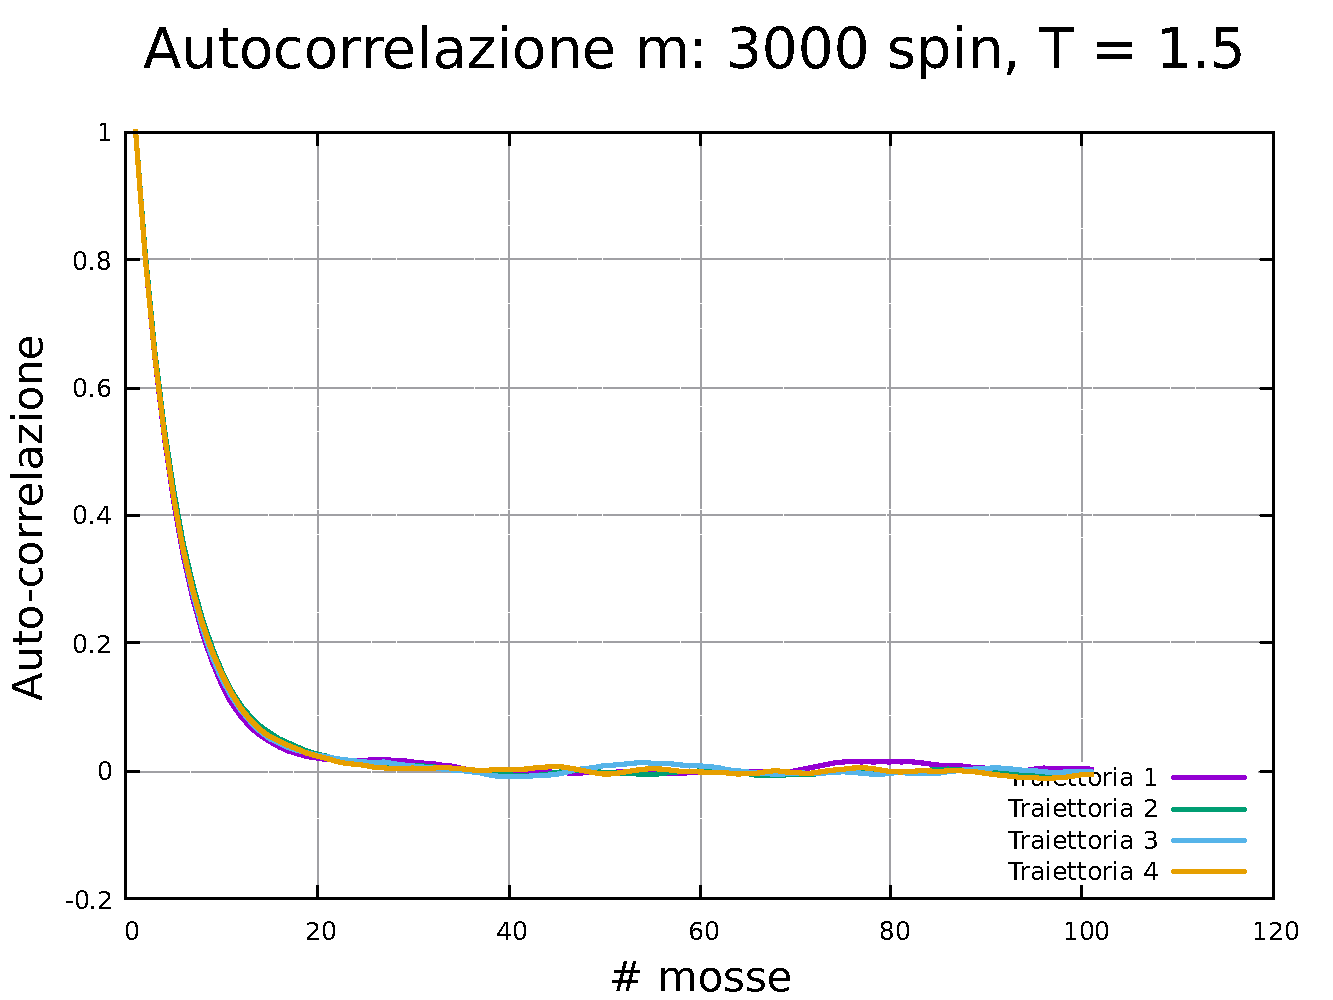
\includegraphics[page=1, width=\textwidth]{Immagini/simIsing1D/magn0.0/tcorr/auto_3000_1.5.pdf}
      \caption{$T\,=\,1.5$}
    \end{minipage}\hfill
    \begin{minipage}{0.45\textwidth}  
      \centering
      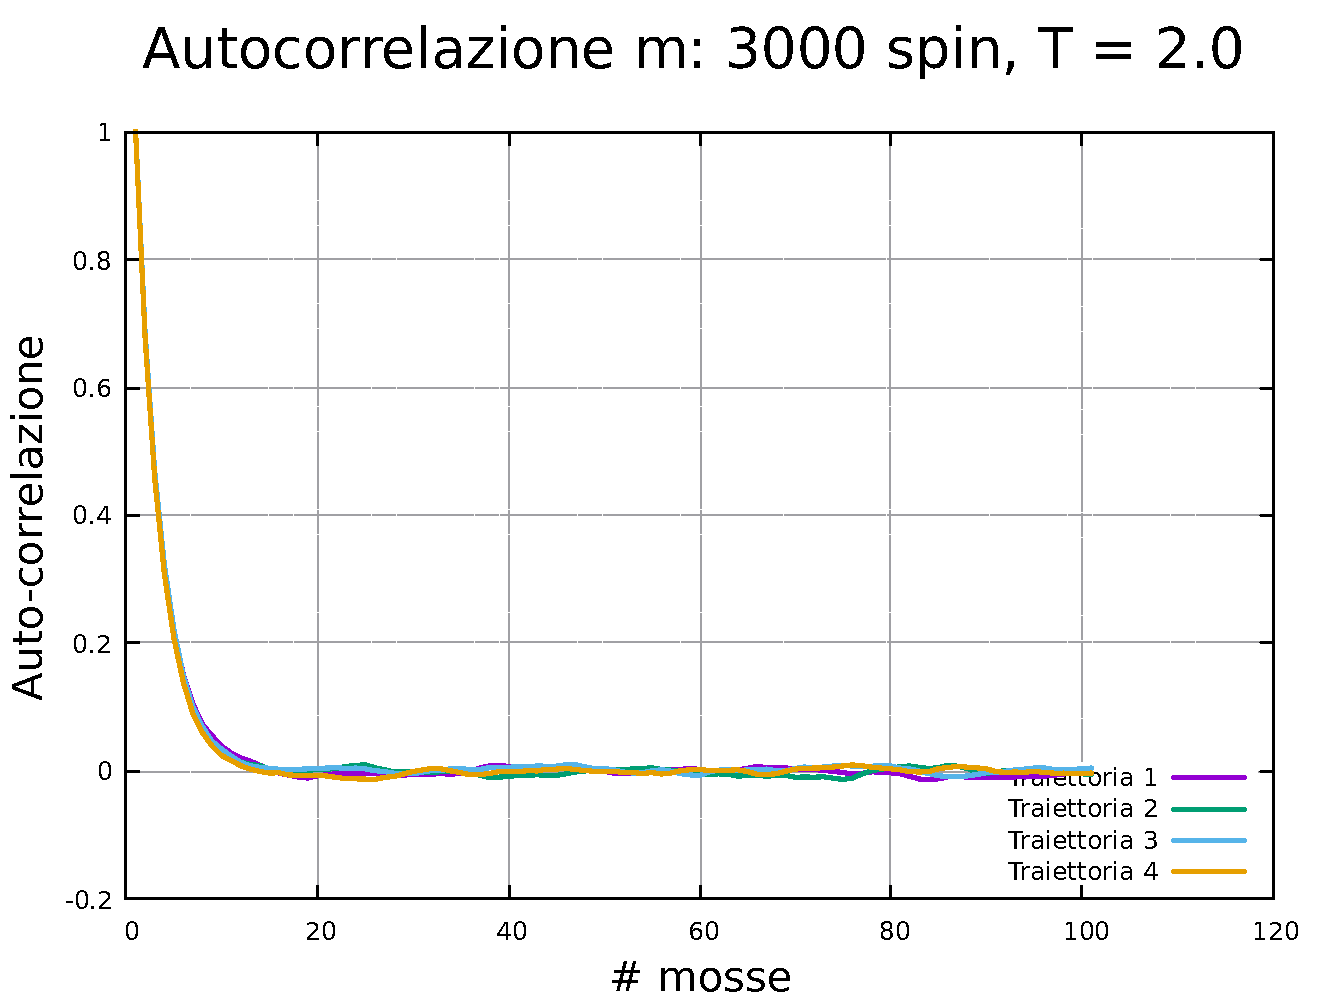
\includegraphics[page=1, width=\textwidth]{Immagini/simIsing1D/magn0.0/tcorr/auto_3000_2.0.pdf}
      \caption{$T\,=\,2.0$}
    \end{minipage}
    \caption{Studio dell'auto-correlazione per un modello di Ising 1D costituito da 3000 spin.}
\end{figure}

\vspace*{\fill}

\newpage

\vspace*{\fill}

\begin{figure}[htbp]
    \centering
    \begin{minipage}{0.45\textwidth}  
      \centering
      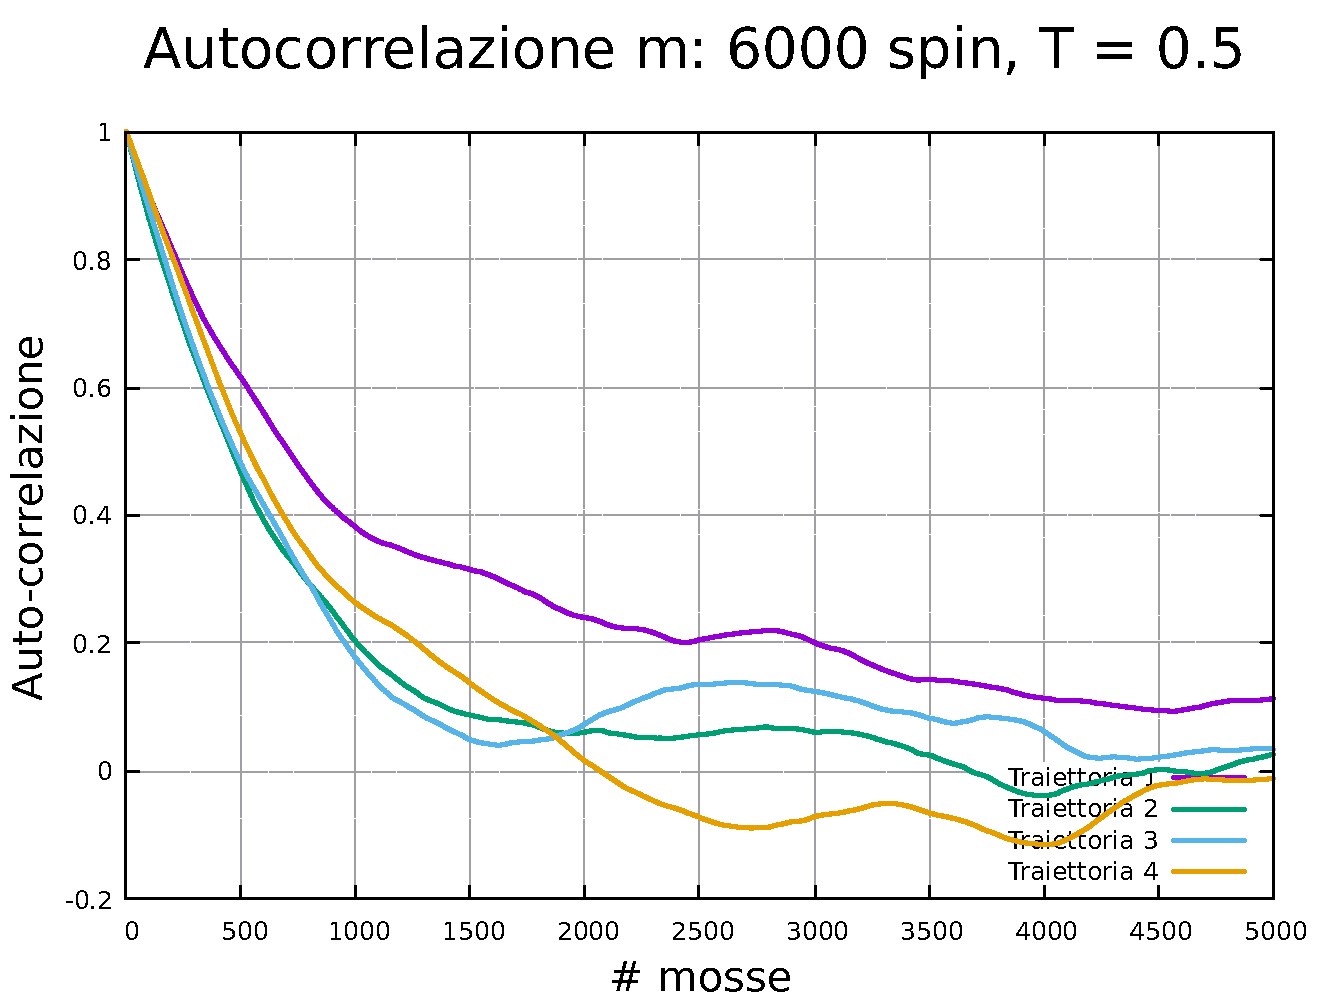
\includegraphics[page=1, width=\textwidth]{Immagini/simIsing1D/magn0.0/tcorr/auto_6000_0.5.pdf}
      \caption{$T\,=\,0.5$}
    \end{minipage}\hfill
    \begin{minipage}{0.45\textwidth}  
      \centering
      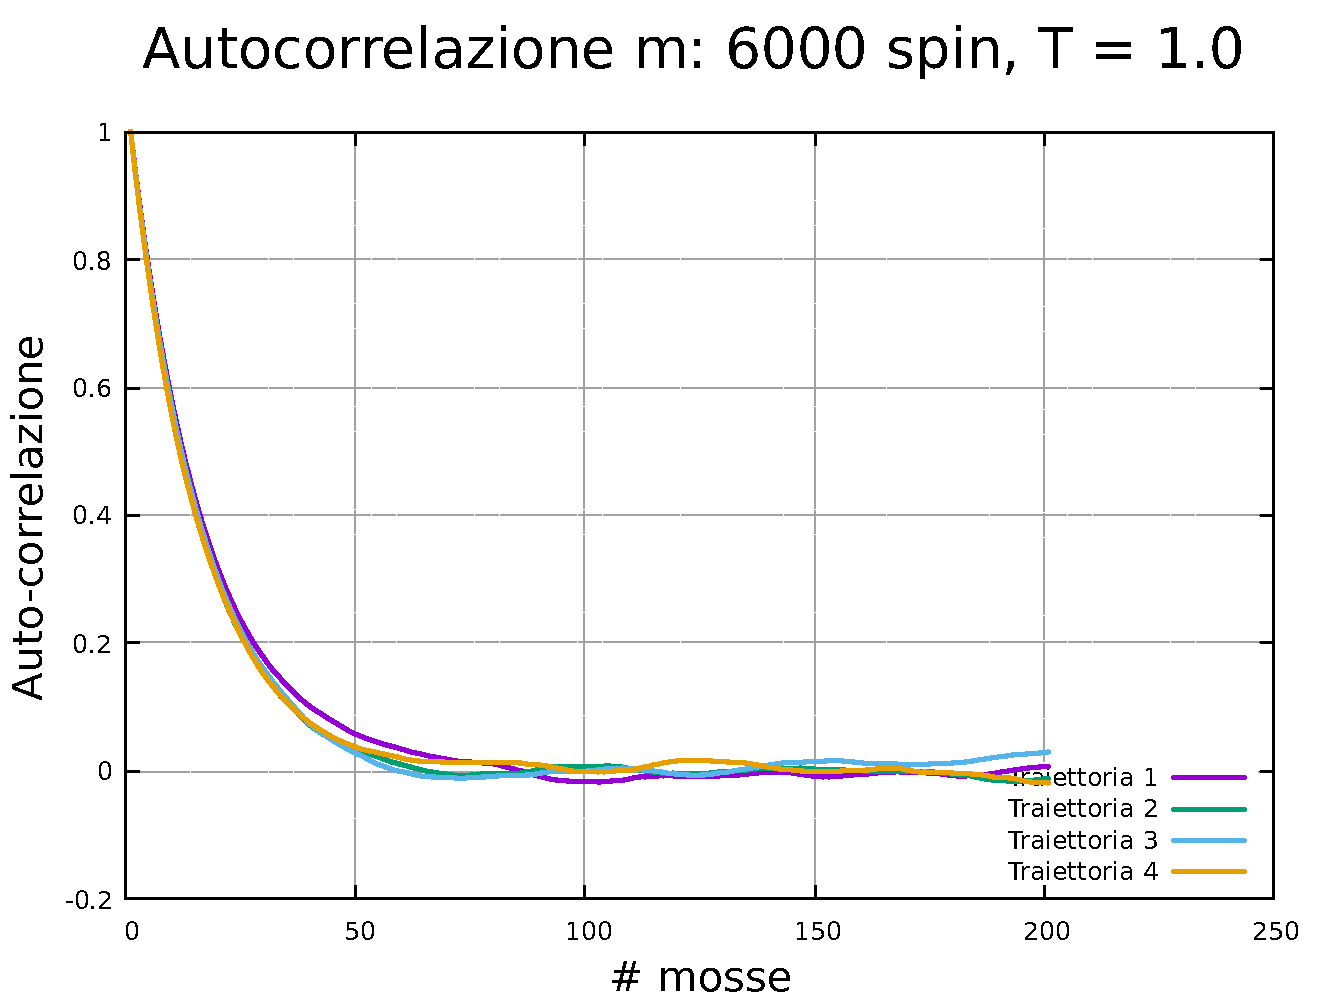
\includegraphics[page=1, width=\textwidth]{Immagini/simIsing1D/magn0.0/tcorr/auto_6000_1.0.pdf}
      \caption{$T\,=\,1.0$}
    \end{minipage}
    \vskip\baselineskip 
  
    \begin{minipage}{0.45\textwidth}  
      \centering
      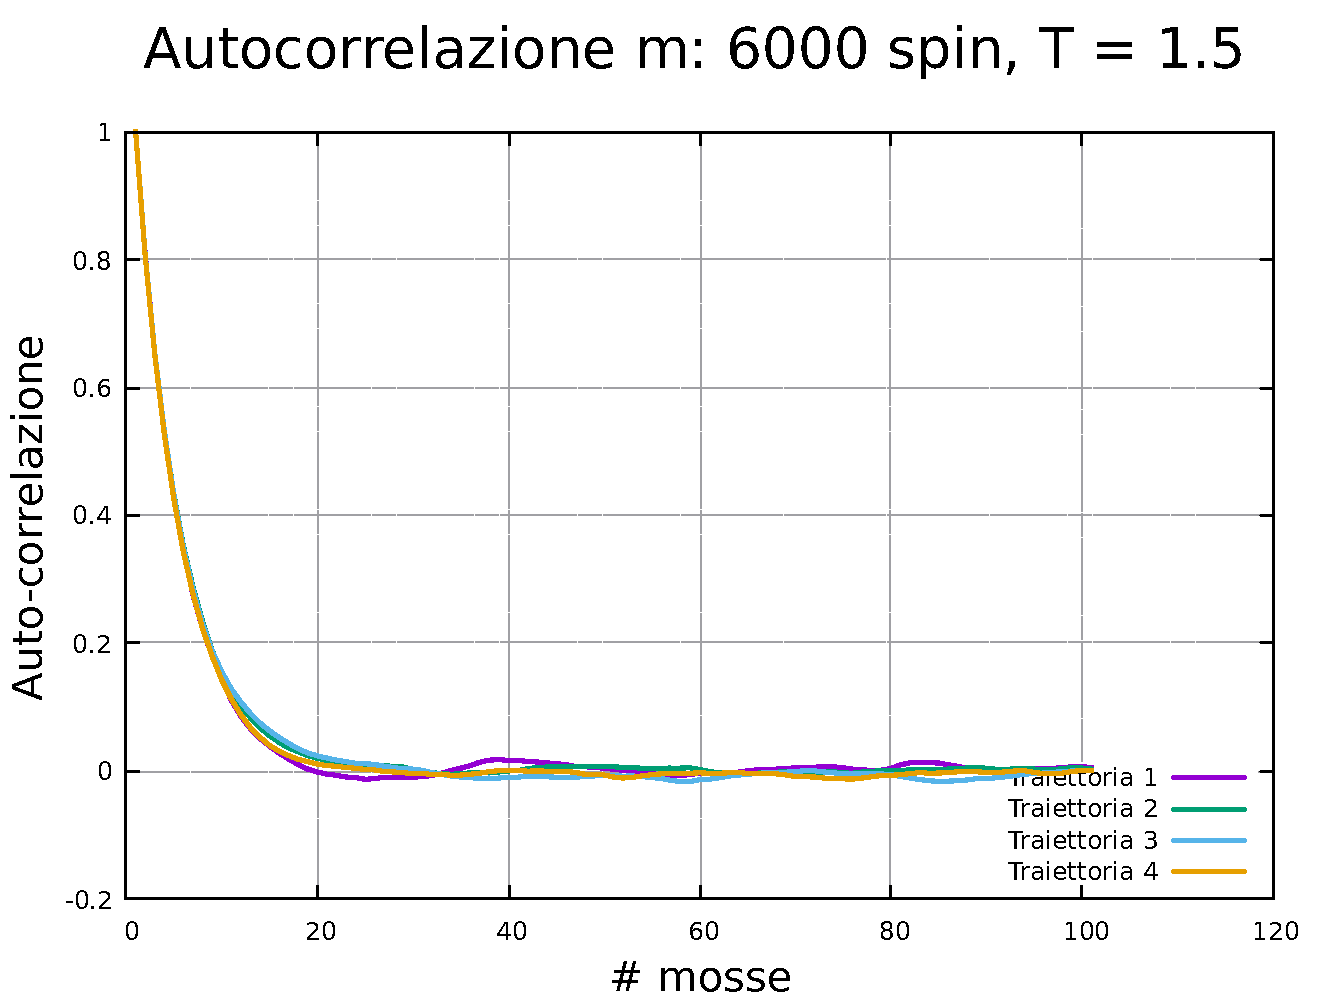
\includegraphics[page=1, width=\textwidth]{Immagini/simIsing1D/magn0.0/tcorr/auto_6000_1.5.pdf}
      \caption{$T\,=\,1.5$}
    \end{minipage}\hfill
    \begin{minipage}{0.45\textwidth}  
      \centering
      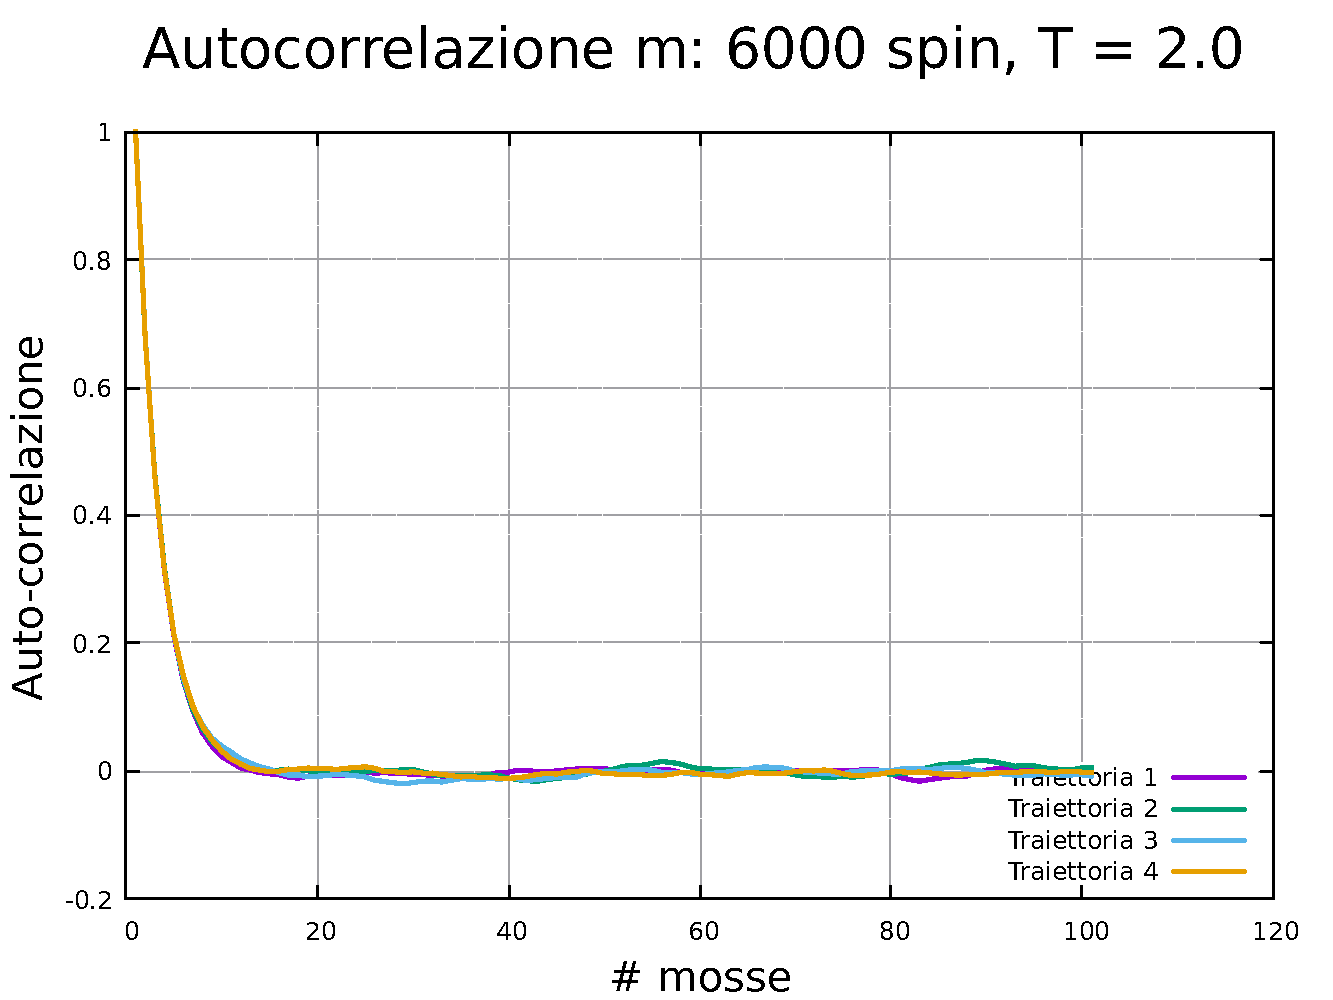
\includegraphics[page=1, width=\textwidth]{Immagini/simIsing1D/magn0.0/tcorr/auto_6000_2.0.pdf}
      \caption{$T\,=\,2.0$}
    \end{minipage}
    \caption{Studio dell'auto-correlazione per un modello di Ising 1D costituito da 6000 spin.}
\end{figure}

\vspace*{\fill}

\newpage

\vspace*{\fill}

\begin{figure}[htbp]
    \centering
    \begin{minipage}{0.45\textwidth}  
      \centering
      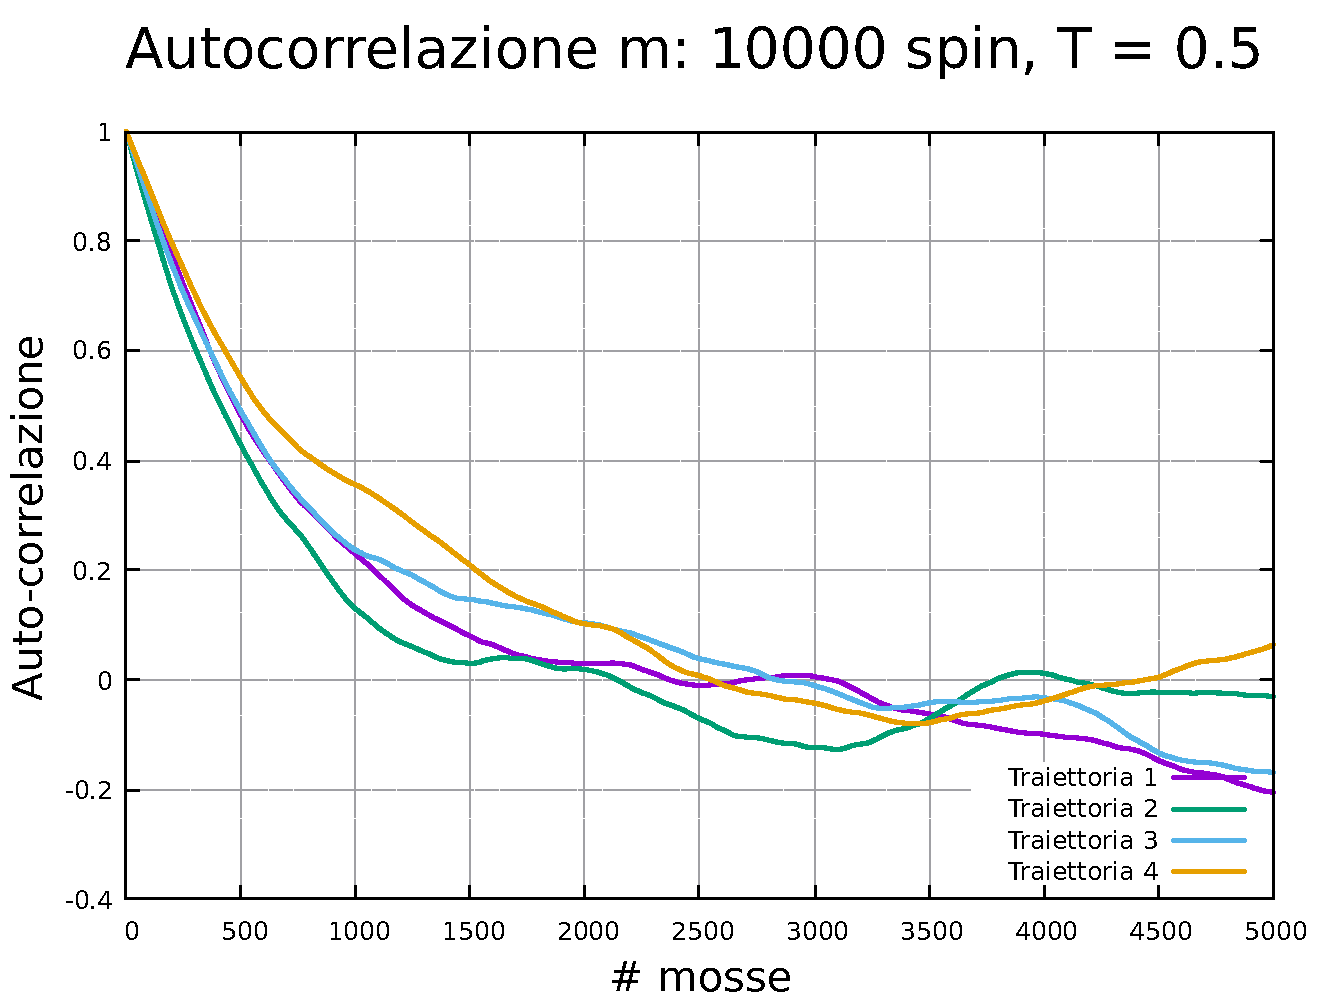
\includegraphics[page=1, width=\textwidth]{Immagini/simIsing1D/magn0.0/tcorr/auto_10000_0.5.pdf}
      \caption{$T\,=\,0.5$}
    \end{minipage}\hfill
    \begin{minipage}{0.45\textwidth}  
      \centering
      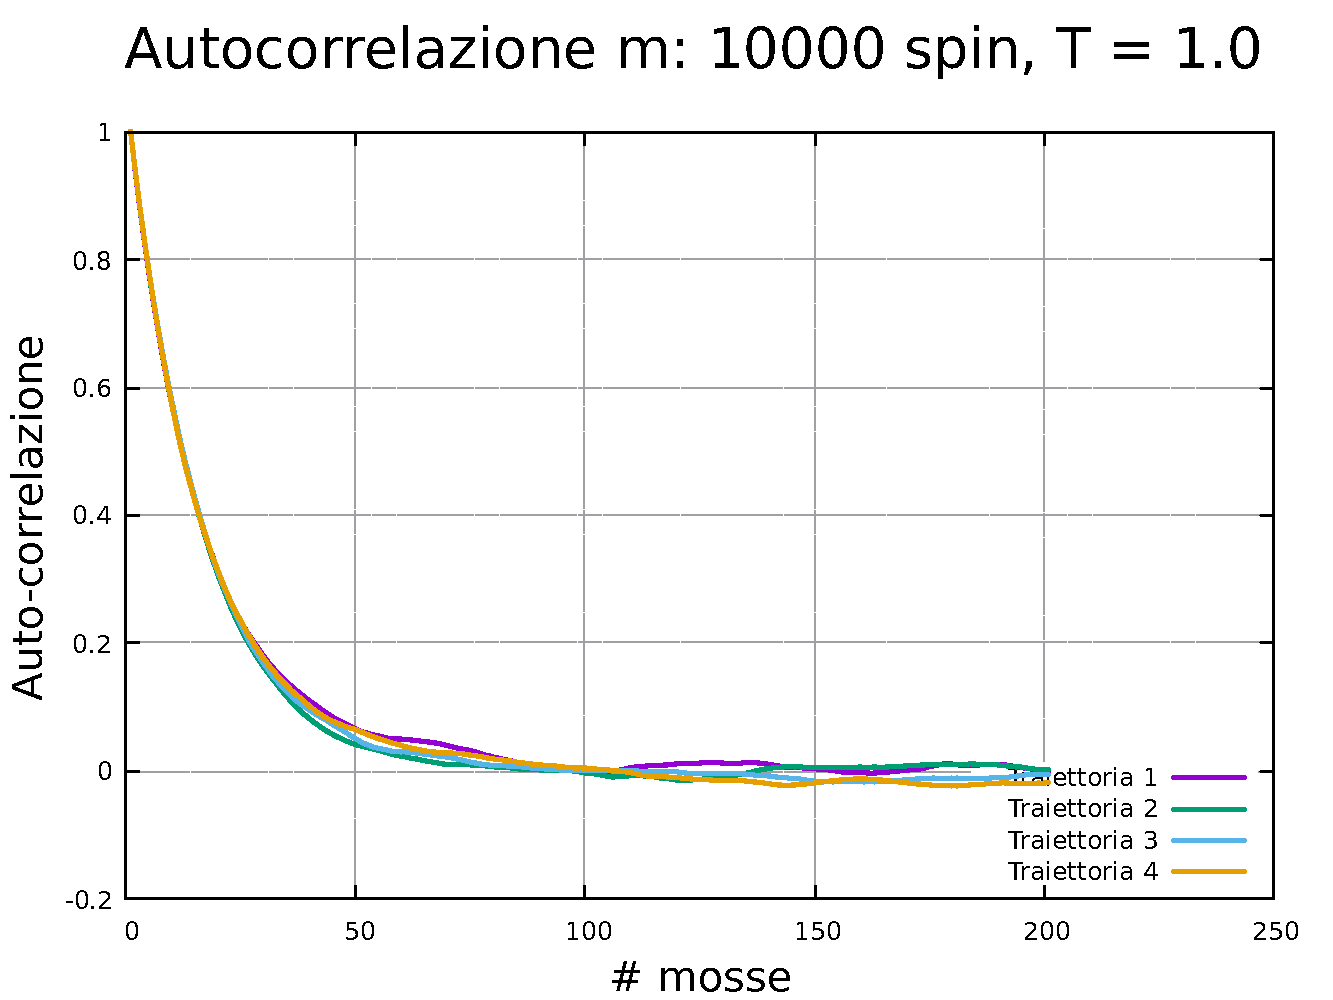
\includegraphics[page=1, width=\textwidth]{Immagini/simIsing1D/magn0.0/tcorr/auto_10000_1.0.pdf}
      \caption{$T\,=\,1.0$}
    \end{minipage}
    \vskip\baselineskip 
  
    \begin{minipage}{0.45\textwidth}  
      \centering
      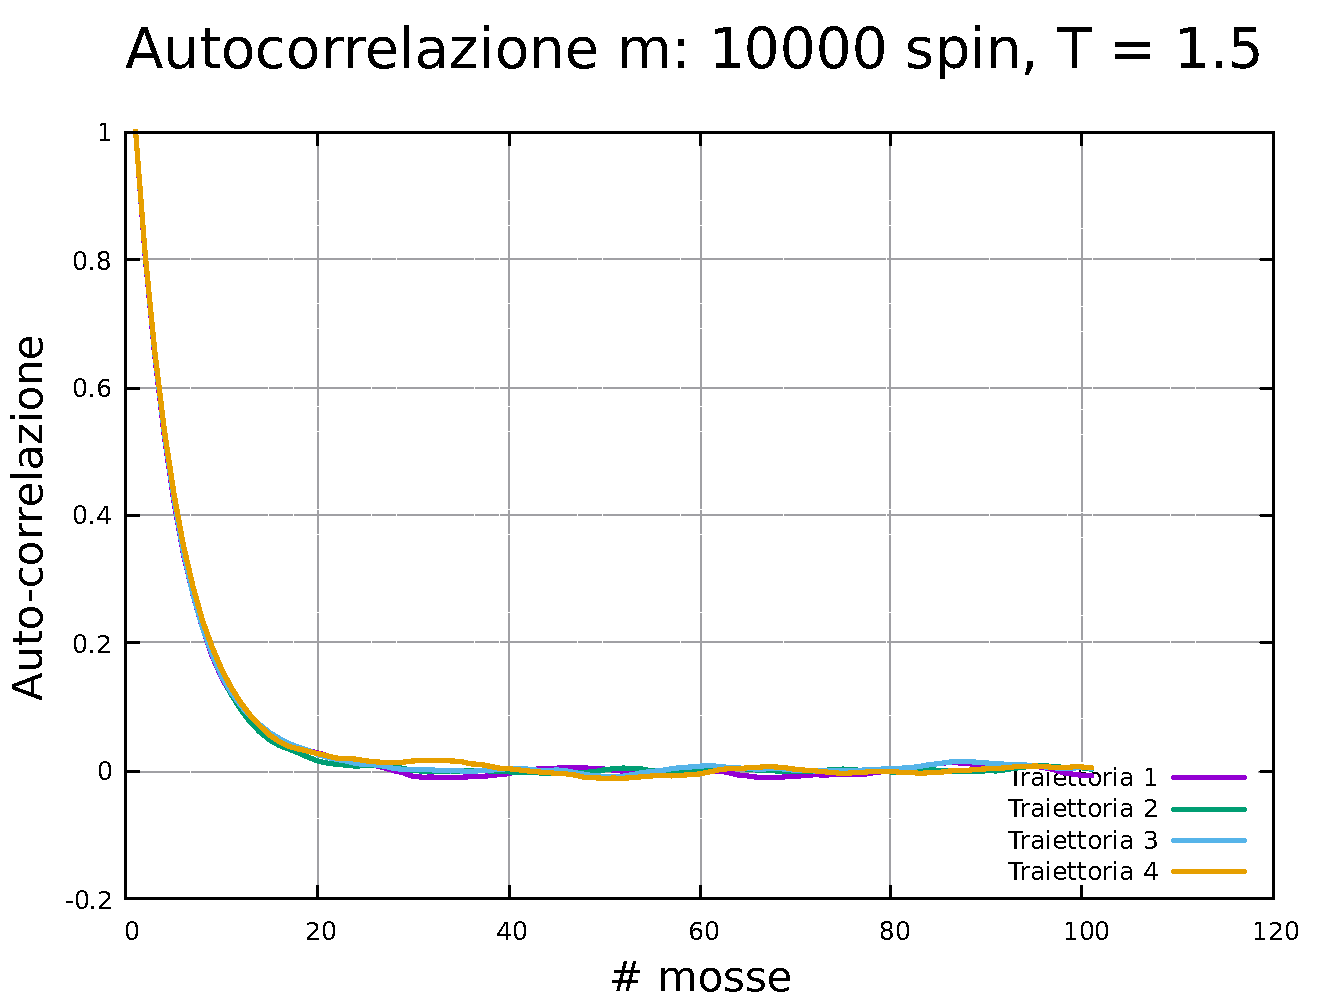
\includegraphics[page=1, width=\textwidth]{Immagini/simIsing1D/magn0.0/tcorr/auto_10000_1.5.pdf}
      \caption{$T\,=\,1.5$}
    \end{minipage}\hfill
    \begin{minipage}{0.45\textwidth}  
      \centering
      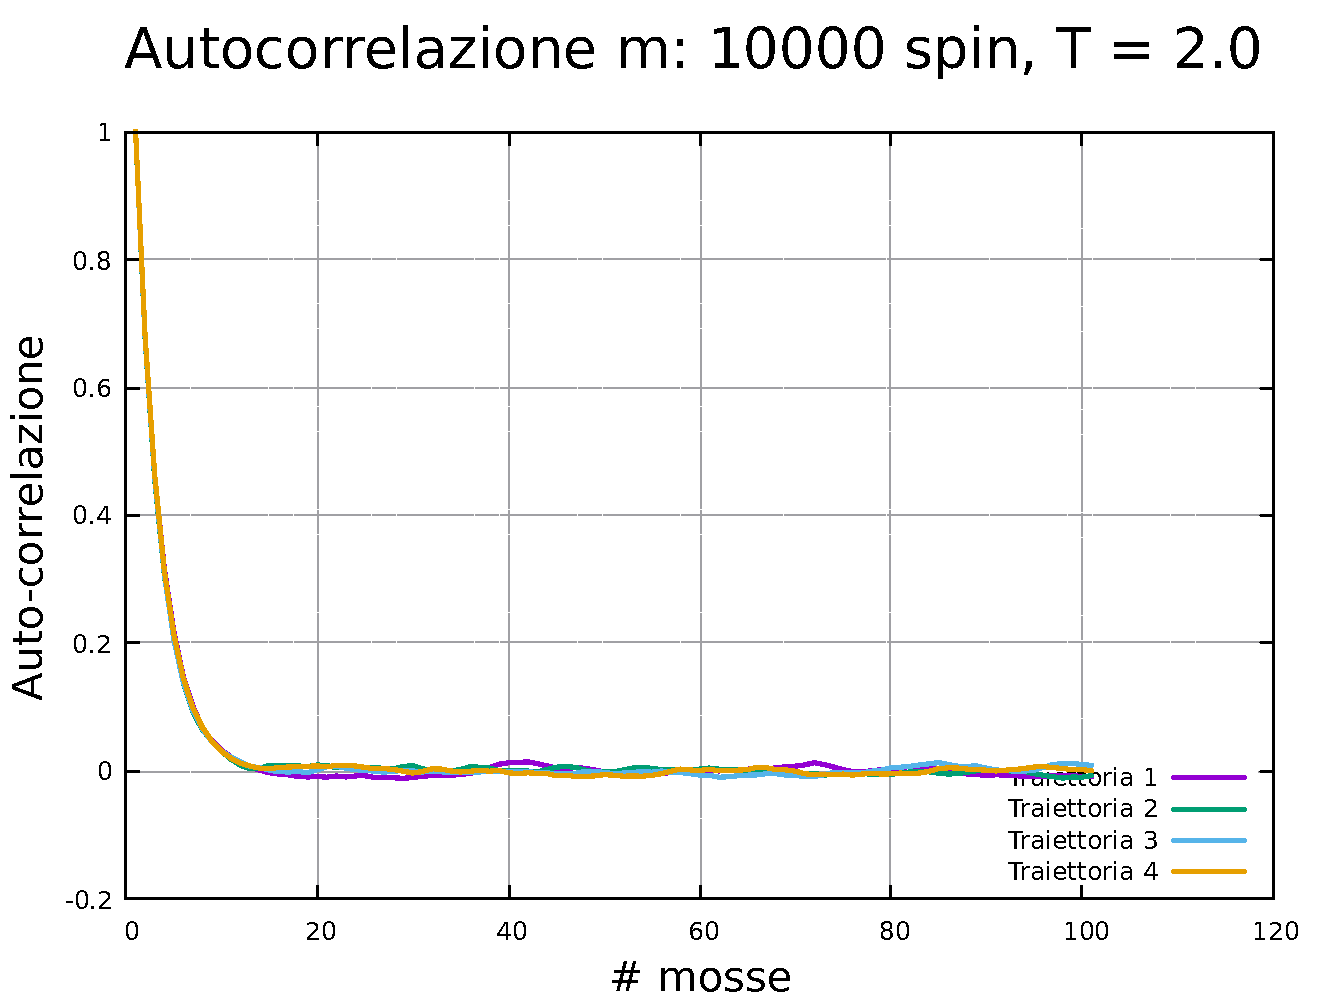
\includegraphics[page=1, width=\textwidth]{Immagini/simIsing1D/magn0.0/tcorr/auto_10000_2.0.pdf}
      \caption{$T\,=\,2.0$}
    \end{minipage}
    \caption{Studio dell'auto-correlazione per un modello di Ising 1D costituito da 10000 spin.}
\end{figure}

\vspace*{\fill}

\newpage



\subsection{Dimensione dei blocchi}

\vspace*{\fill}

\begin{figure}[htbp]
    \centering
    \begin{minipage}{0.45\textwidth}  
      \centering
      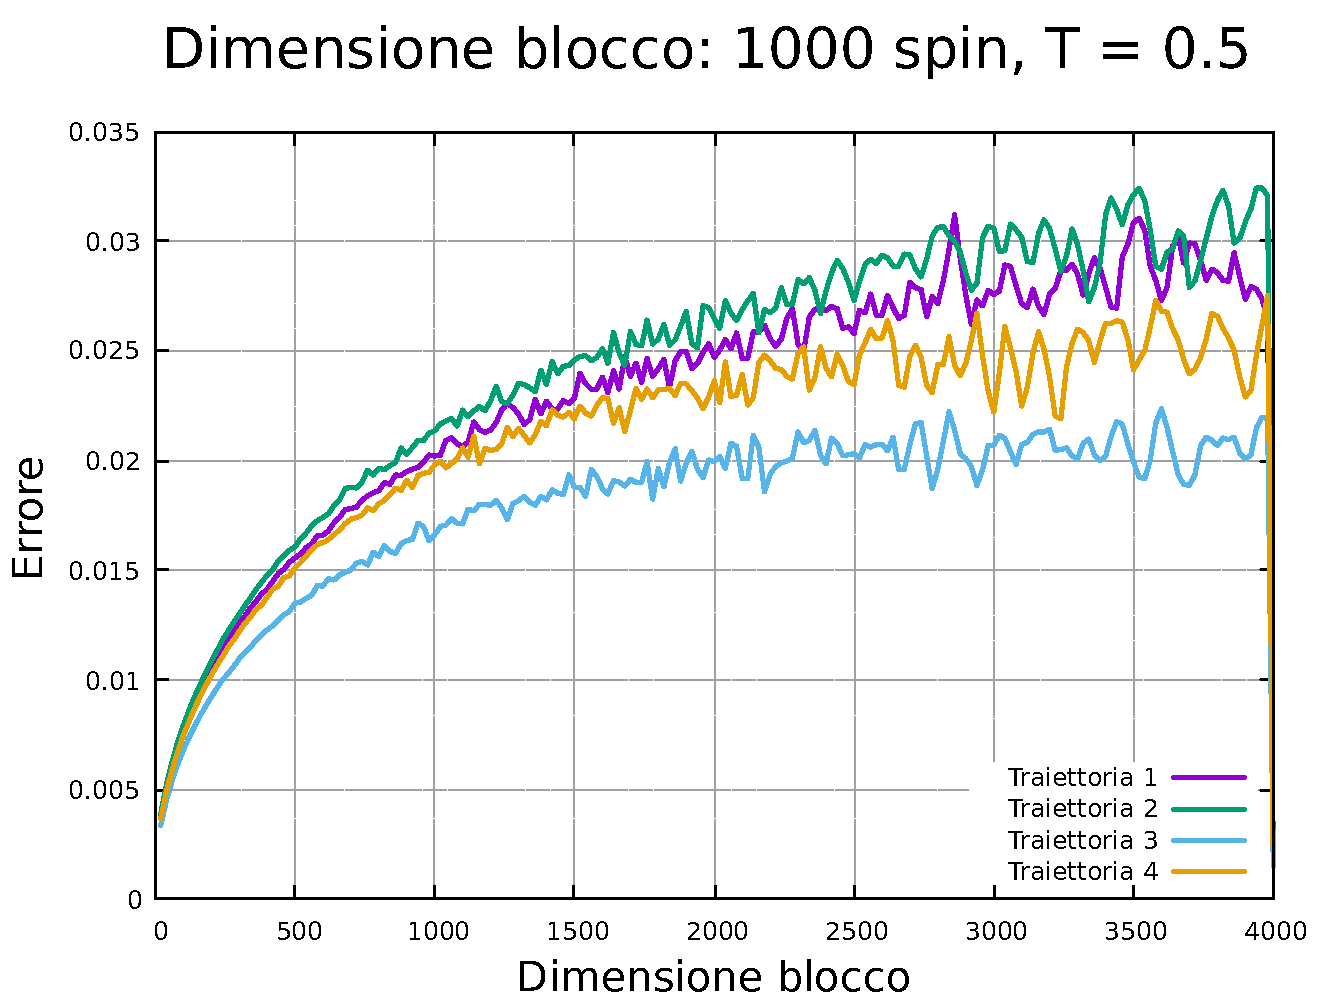
\includegraphics[page=1, width=\textwidth]{Immagini/simIsing1D/magn0.0/lblk/err_1000_0.5.pdf}
      \caption{$T\,=\,0.5$}
    \end{minipage}\hfill
    \begin{minipage}{0.45\textwidth}  
      \centering
      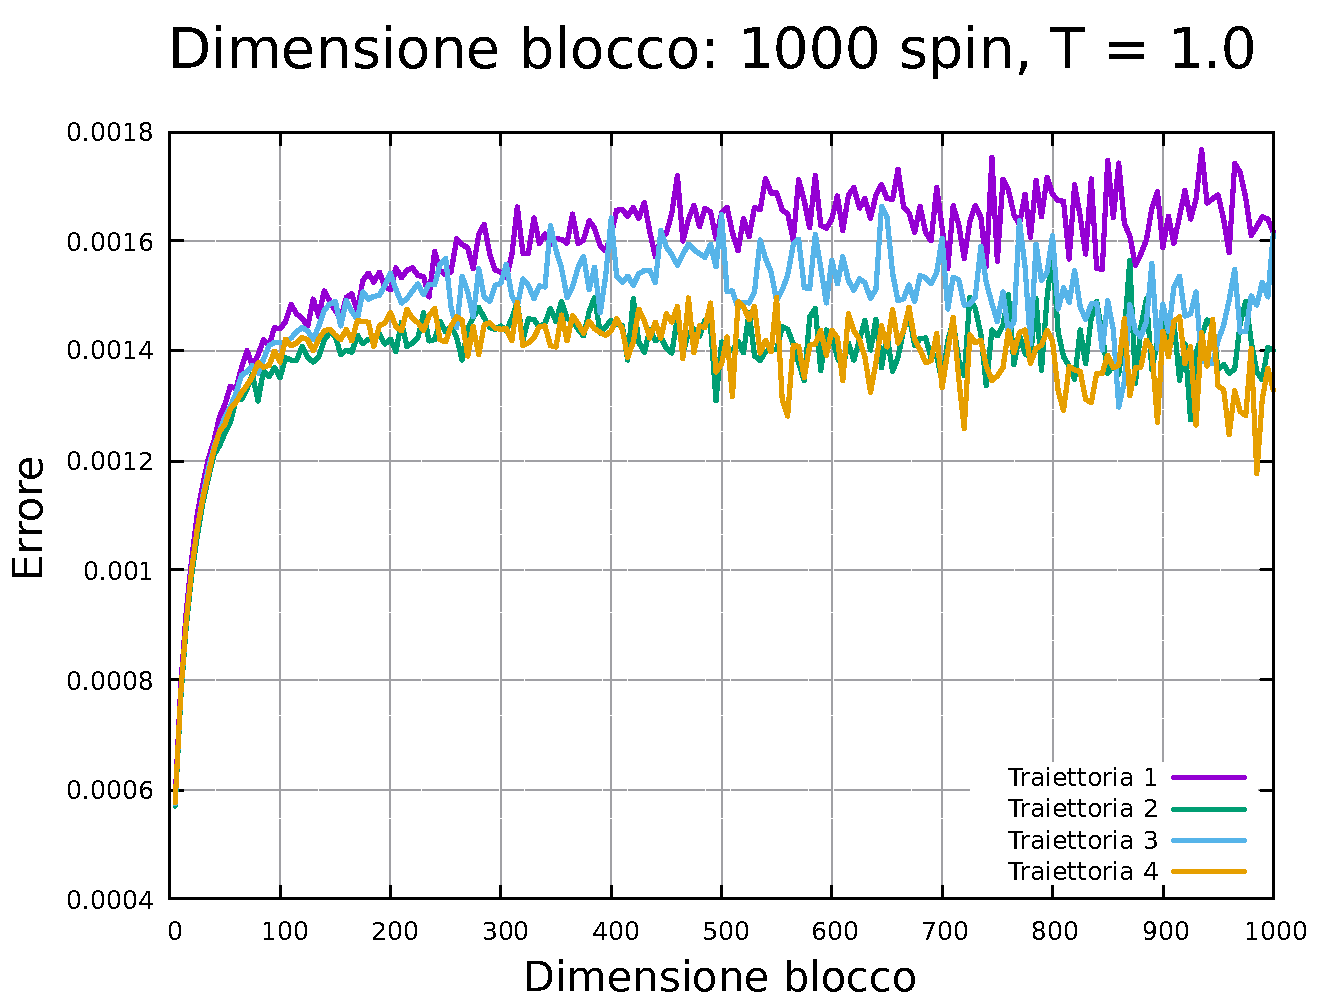
\includegraphics[page=1, width=\textwidth]{Immagini/simIsing1D/magn0.0/lblk/err_1000_1.0.pdf}
      \caption{$T\,=\,1.0$}
    \end{minipage}
    \vskip\baselineskip 
  
    \begin{minipage}{0.45\textwidth}  
      \centering
      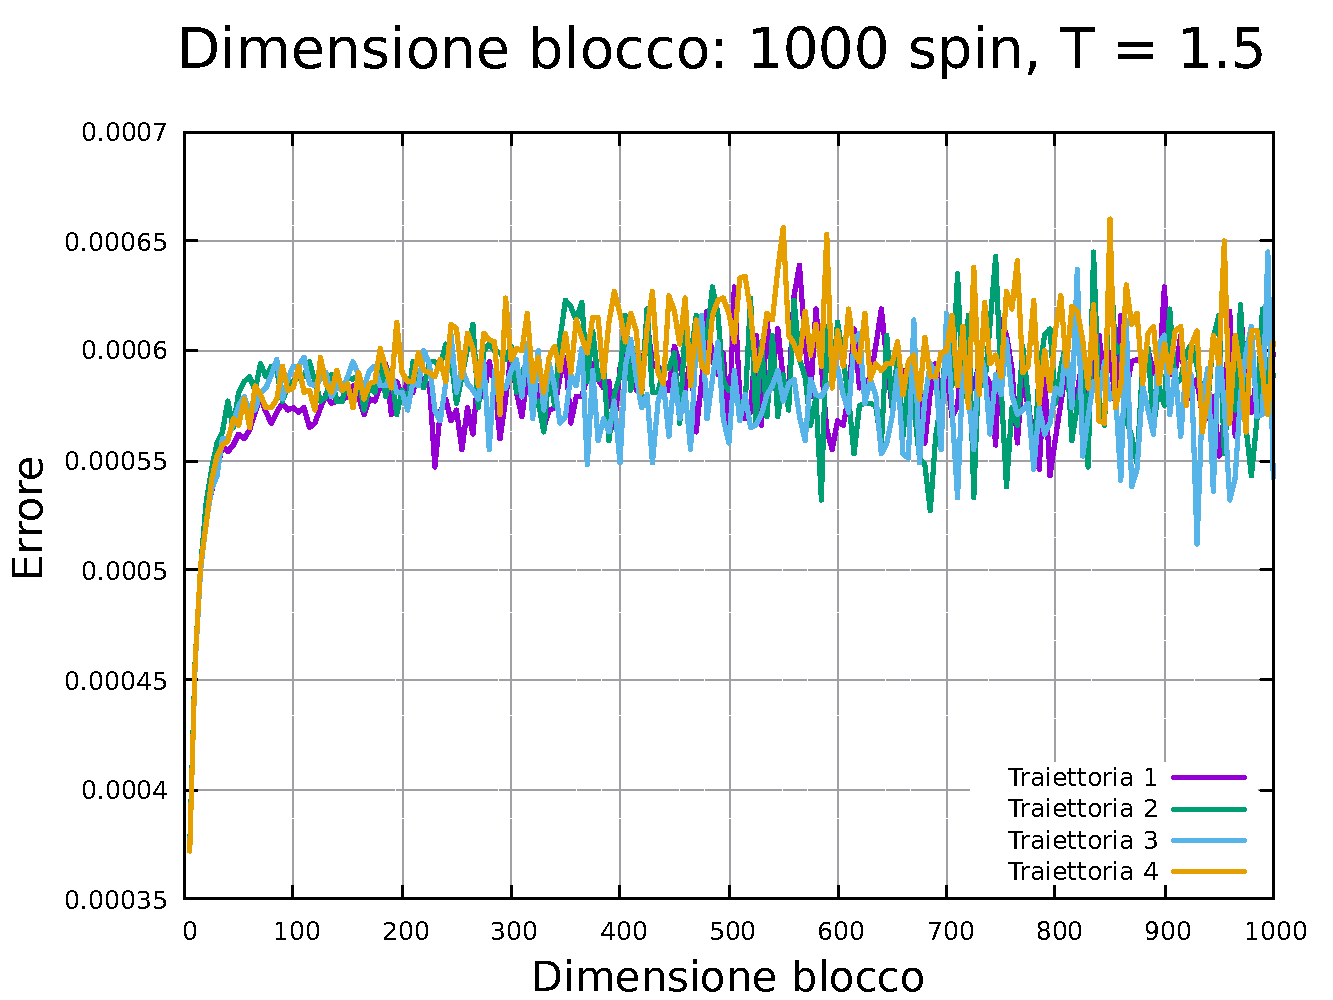
\includegraphics[page=1, width=\textwidth]{Immagini/simIsing1D/magn0.0/lblk/err_1000_1.5.pdf}
      \caption{$T\,=\,1.5$}
    \end{minipage}\hfill
    \begin{minipage}{0.45\textwidth}  
      \centering
      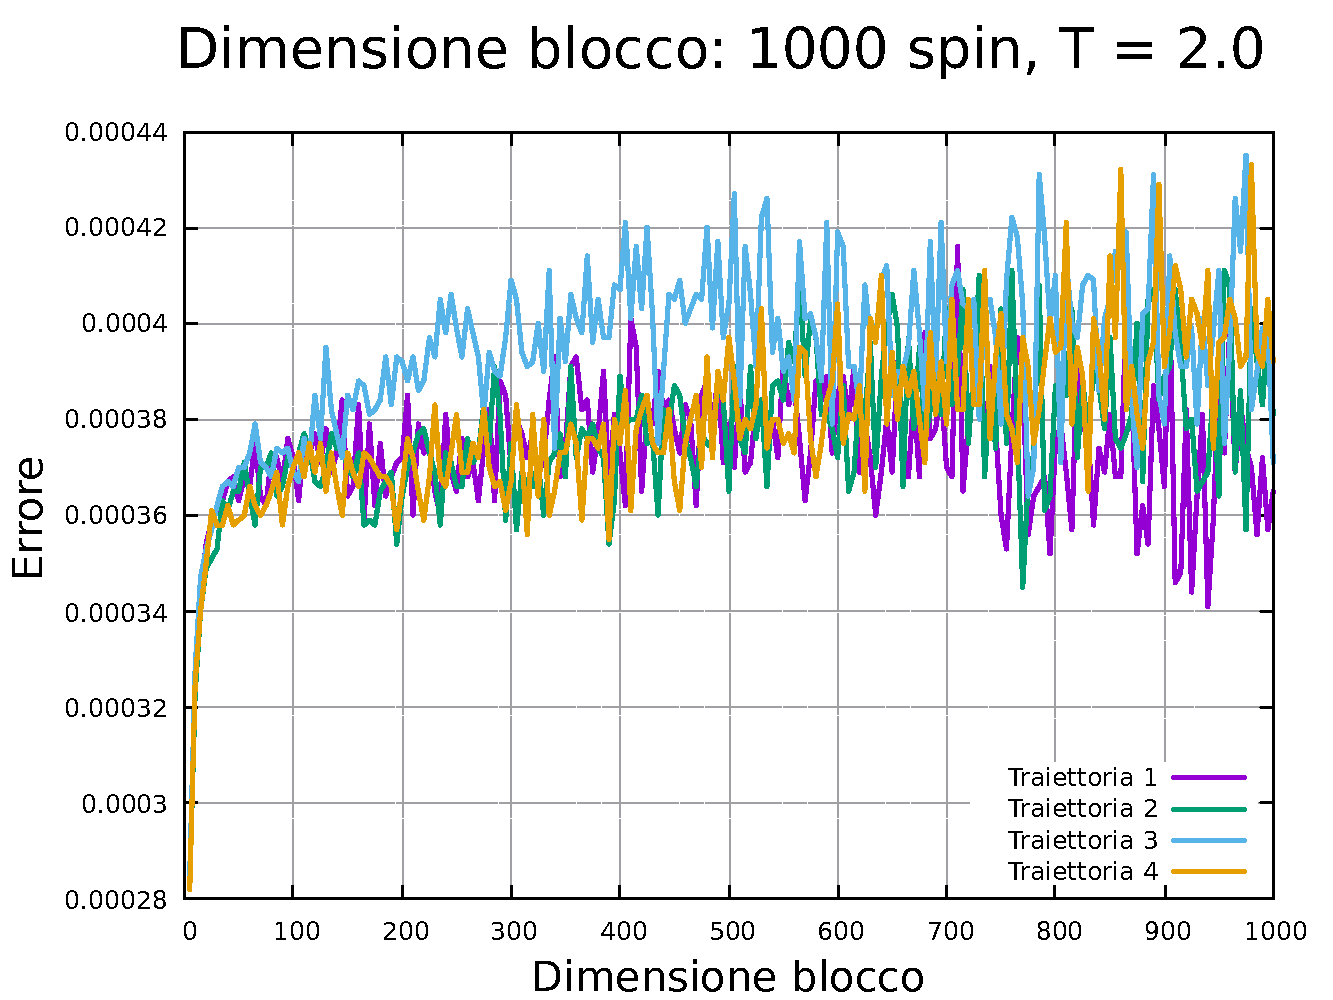
\includegraphics[page=1, width=\textwidth]{Immagini/simIsing1D/magn0.0/lblk/err_1000_2.0.pdf}
      \caption{$T\,=\,2.0$}
    \end{minipage}
    \caption{Errore in funzione della lunghezza dei blocchi per un modello di Ising 1D costituito da 1000 spin.}
\end{figure}

\vspace*{\fill}

\newpage

\vspace*{\fill}

\begin{figure}[htbp]
    \centering
    \begin{minipage}{0.45\textwidth}  
      \centering
      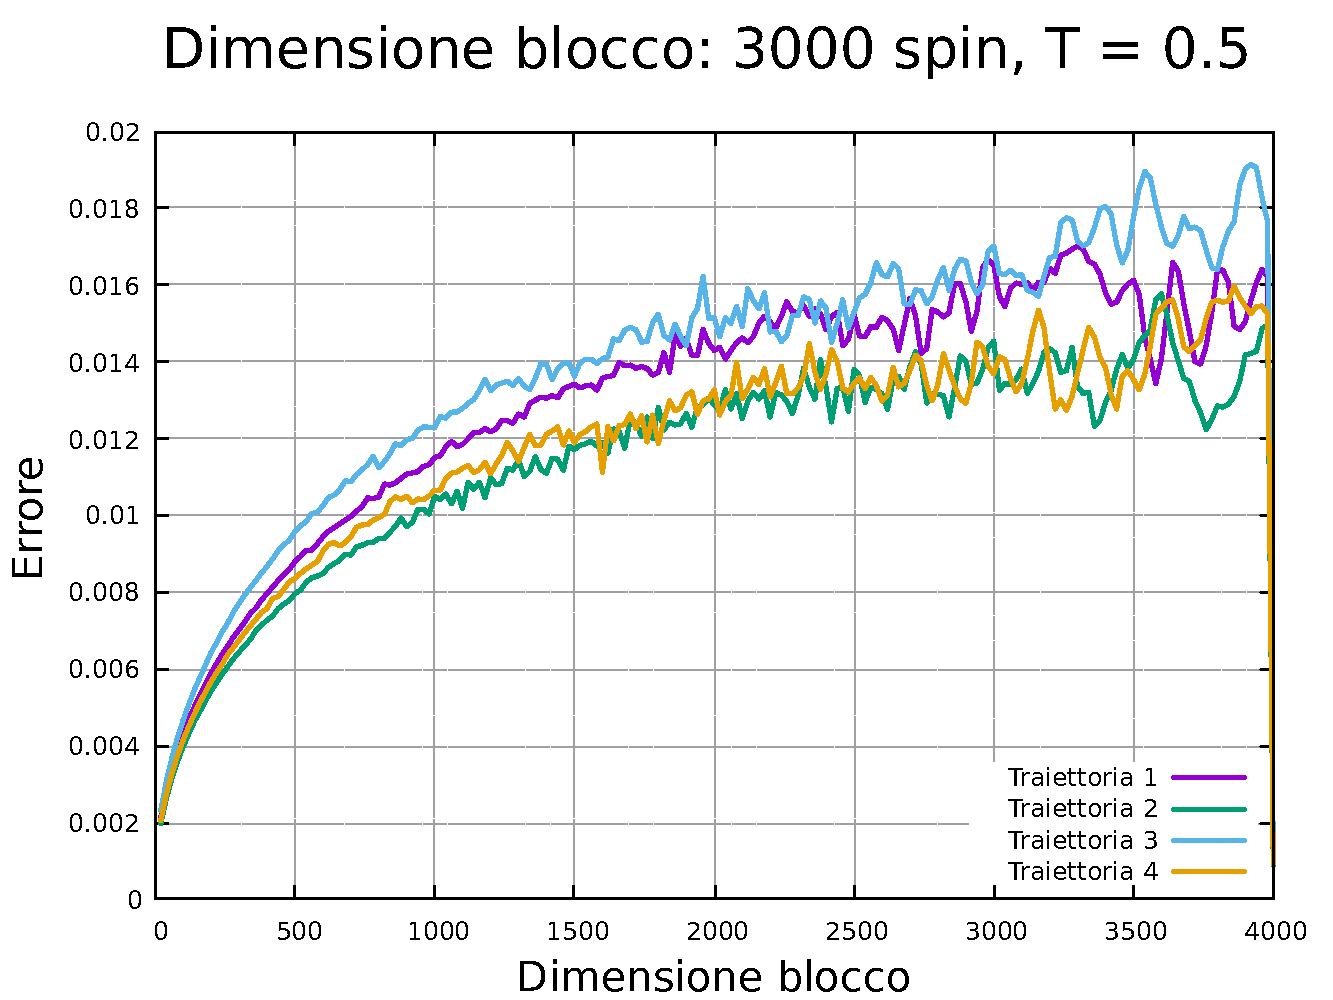
\includegraphics[page=1, width=\textwidth]{Immagini/simIsing1D/magn0.0/lblk/err_3000_0.5.pdf}
      \caption{$T\,=\,0.5$}
    \end{minipage}\hfill
    \begin{minipage}{0.45\textwidth}  
      \centering
      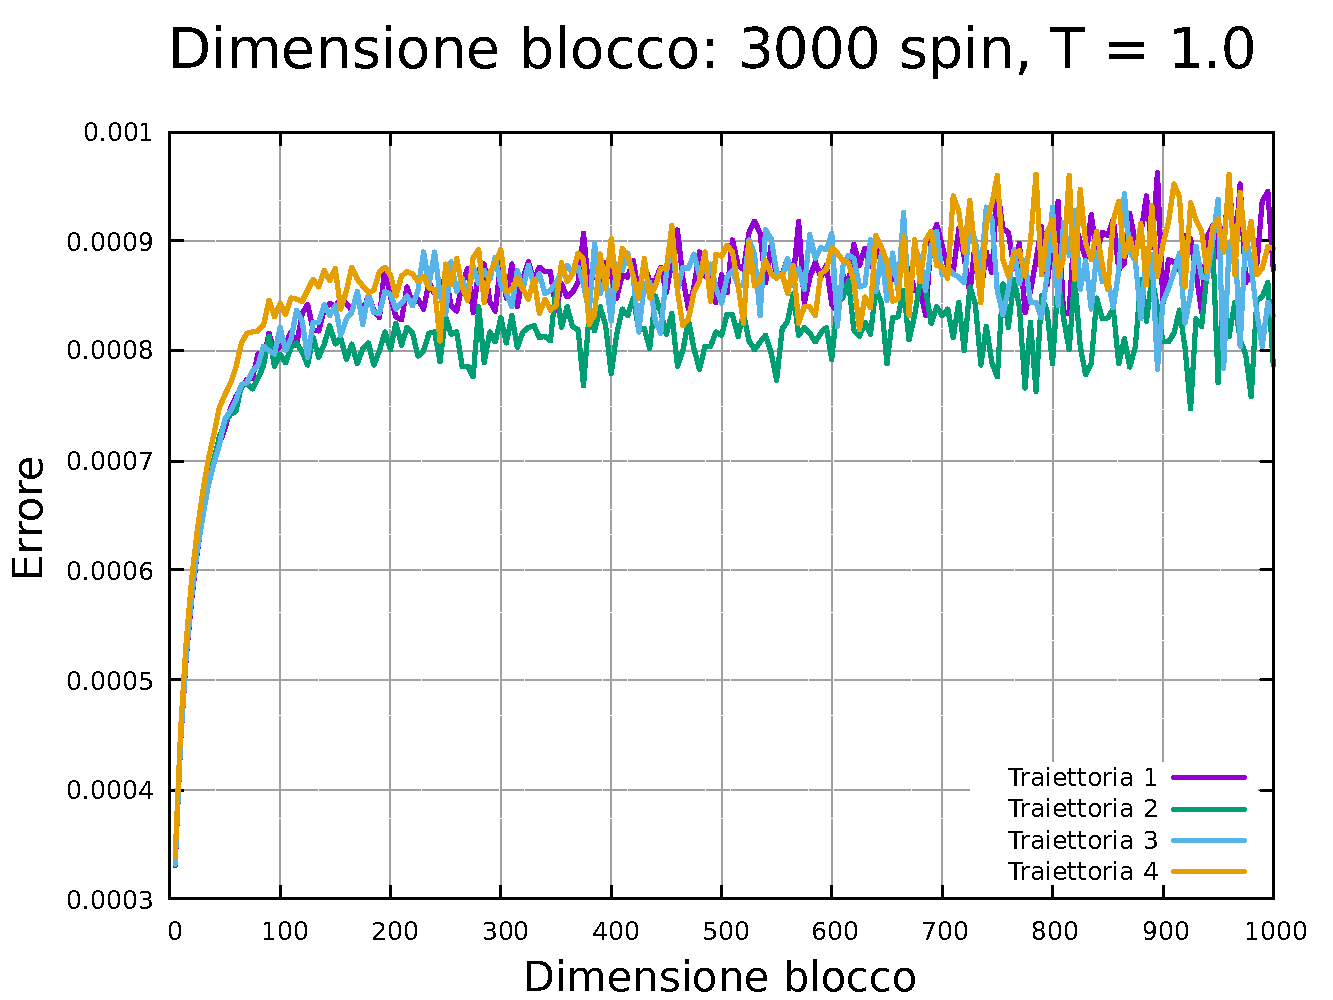
\includegraphics[page=1, width=\textwidth]{Immagini/simIsing1D/magn0.0/lblk/err_3000_1.0.pdf}
      \caption{$T\,=\,1.0$}
    \end{minipage}
    \vskip\baselineskip 
  
    \begin{minipage}{0.45\textwidth}  
      \centering
      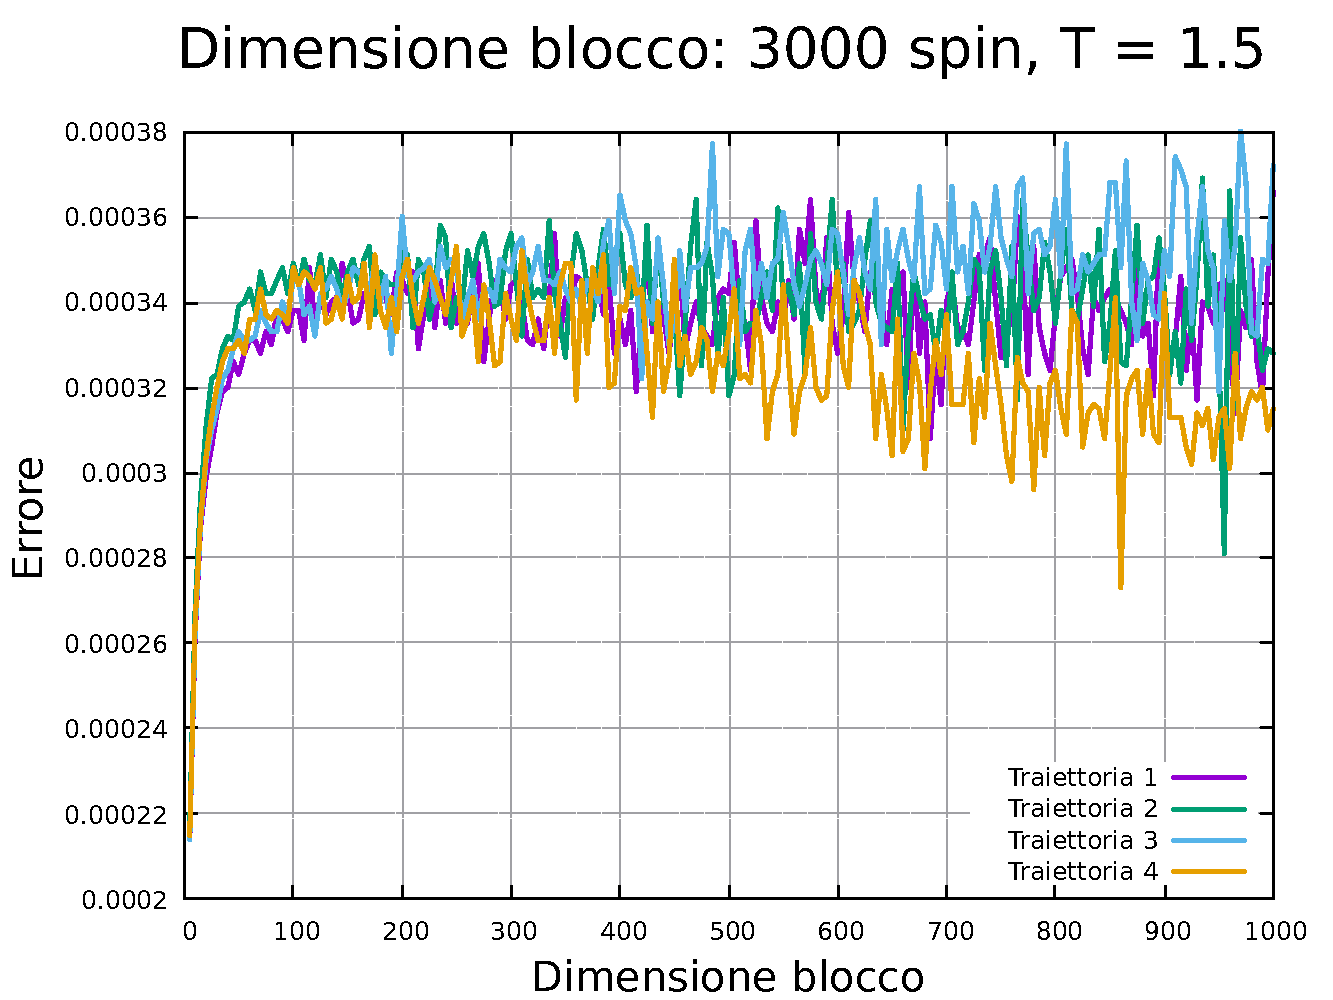
\includegraphics[page=1, width=\textwidth]{Immagini/simIsing1D/magn0.0/lblk/err_3000_1.5.pdf}
      \caption{$T\,=\,1.5$}
    \end{minipage}\hfill
    \begin{minipage}{0.45\textwidth}  
      \centering
      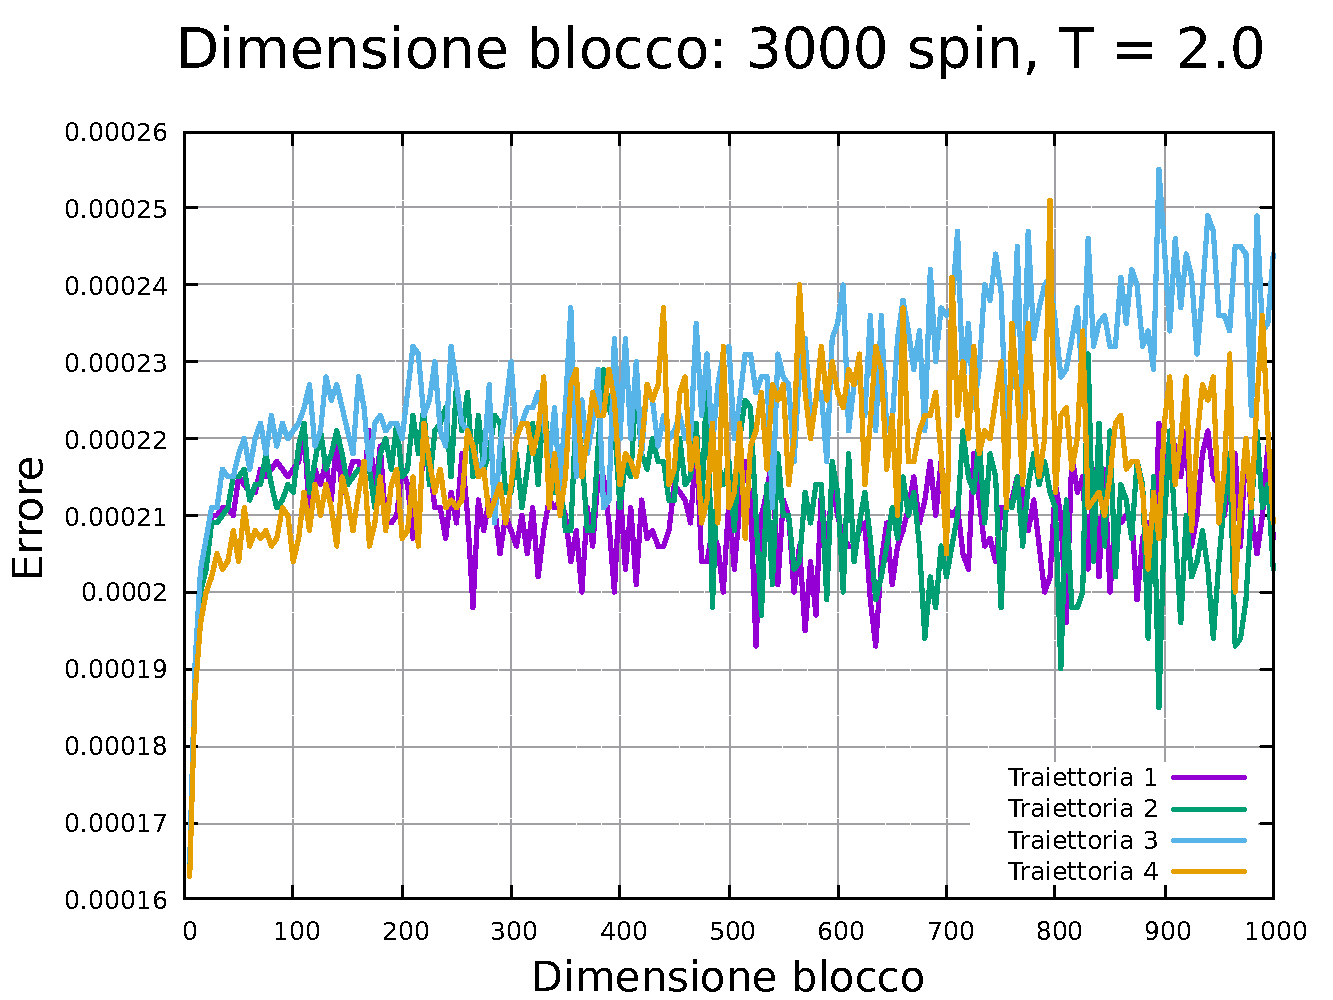
\includegraphics[page=1, width=\textwidth]{Immagini/simIsing1D/magn0.0/lblk/err_3000_2.0.pdf}
      \caption{$T\,=\,2.0$}
    \end{minipage}
    \caption{Errore in funzione della lunghezza dei blocchi per un modello di Ising 1D costituito da 3000 spin.}
\end{figure}

\vspace*{\fill}

\newpage

\vspace*{\fill}

\begin{figure}[htbp]
    \centering
    \begin{minipage}{0.45\textwidth}  
      \centering
      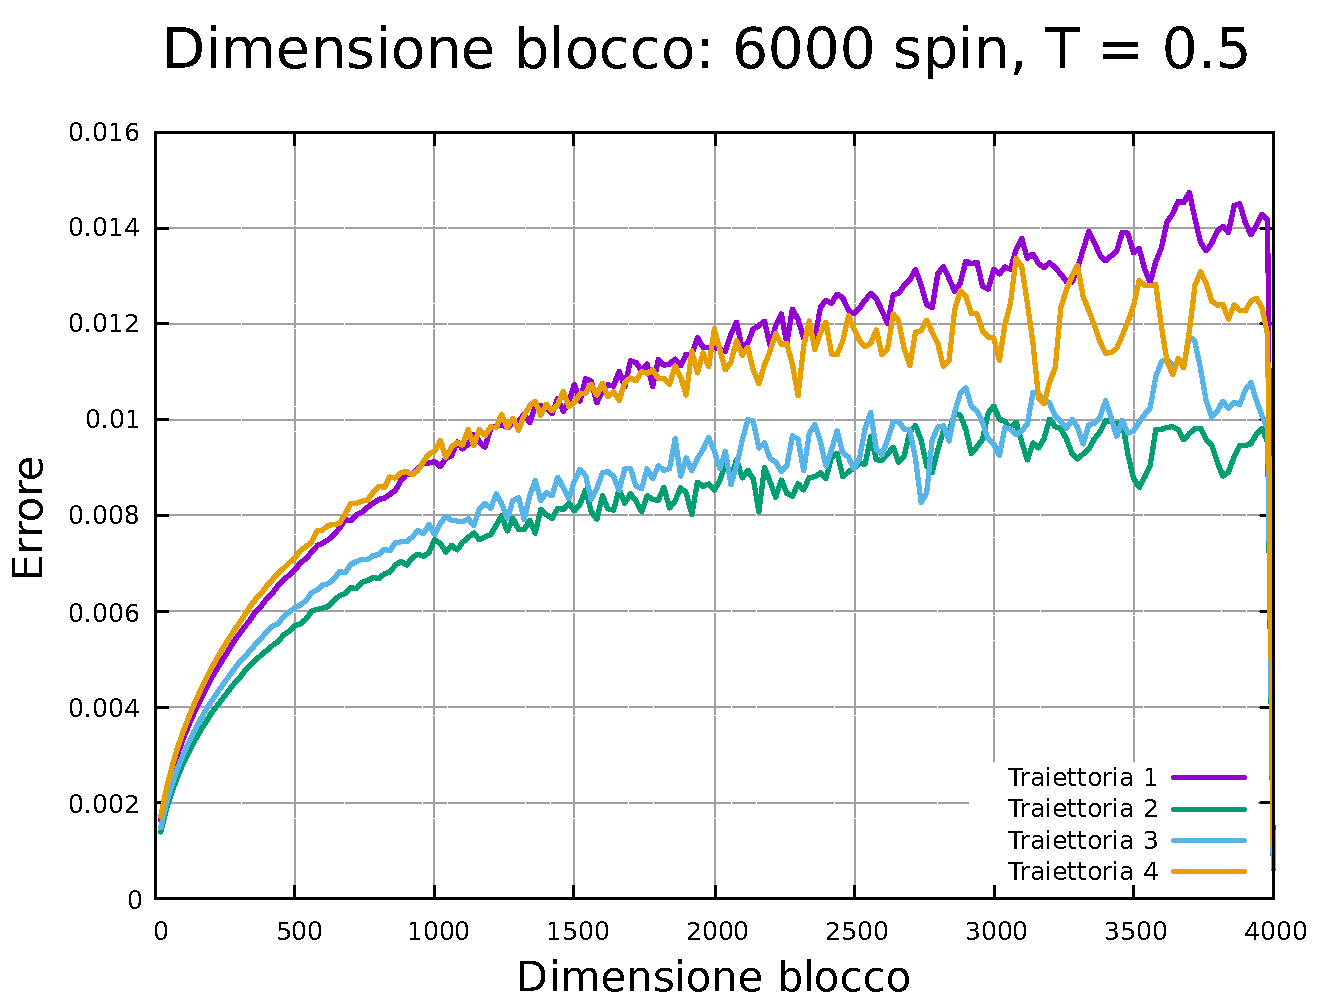
\includegraphics[page=1, width=\textwidth]{Immagini/simIsing1D/magn0.0/lblk/err_6000_0.5.pdf}
      \caption{$T\,=\,0.5$}
    \end{minipage}\hfill
    \begin{minipage}{0.45\textwidth}  
      \centering
      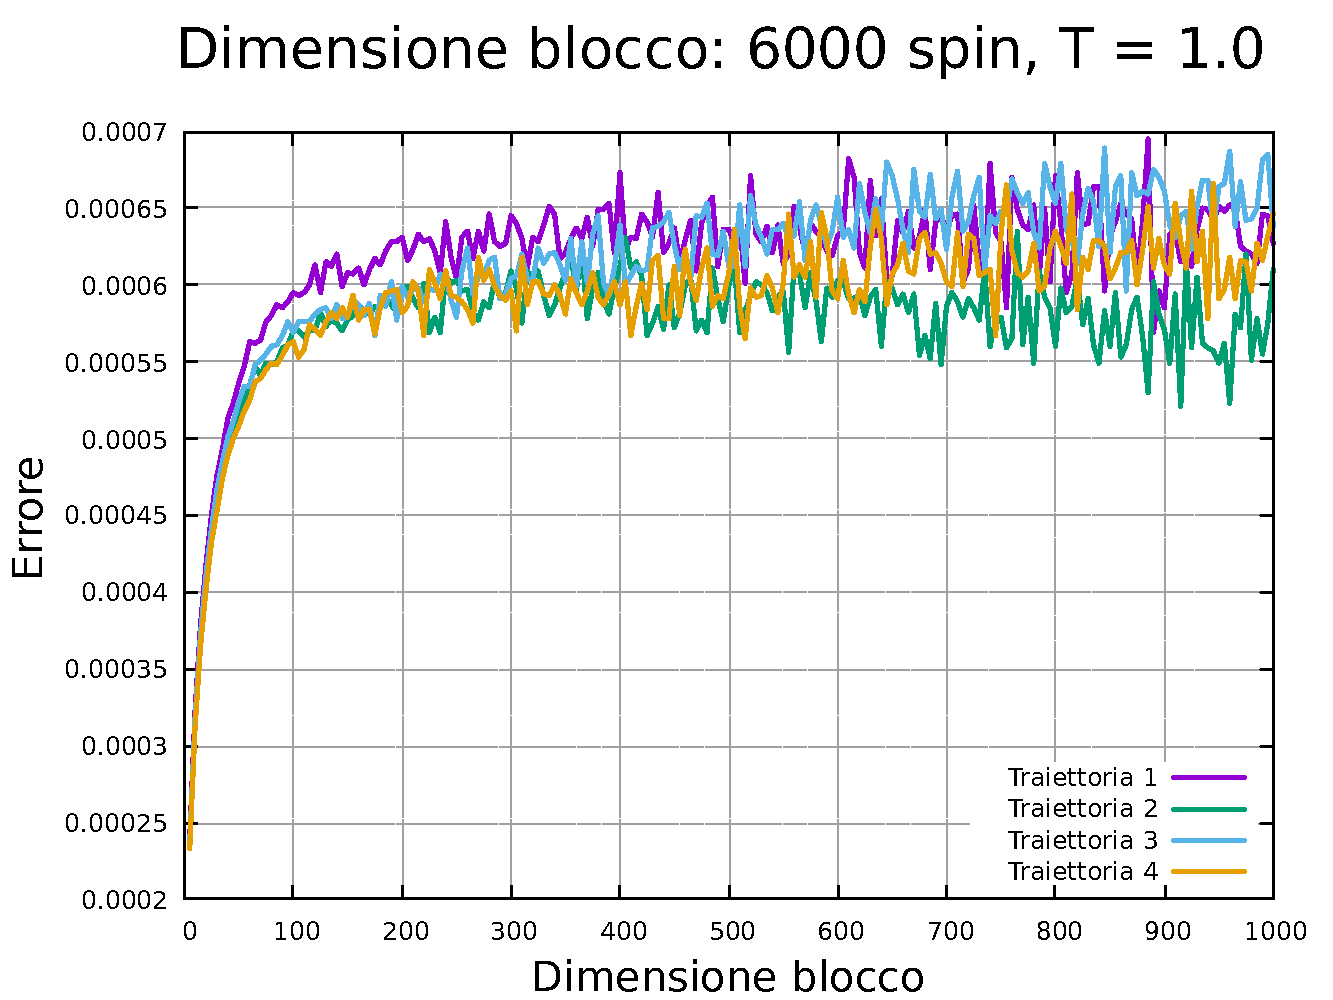
\includegraphics[page=1, width=\textwidth]{Immagini/simIsing1D/magn0.0/lblk/err_6000_1.0.pdf}
      \caption{$T\,=\,1.0$}
    \end{minipage}
    \vskip\baselineskip 
  
    \begin{minipage}{0.45\textwidth}  
      \centering
      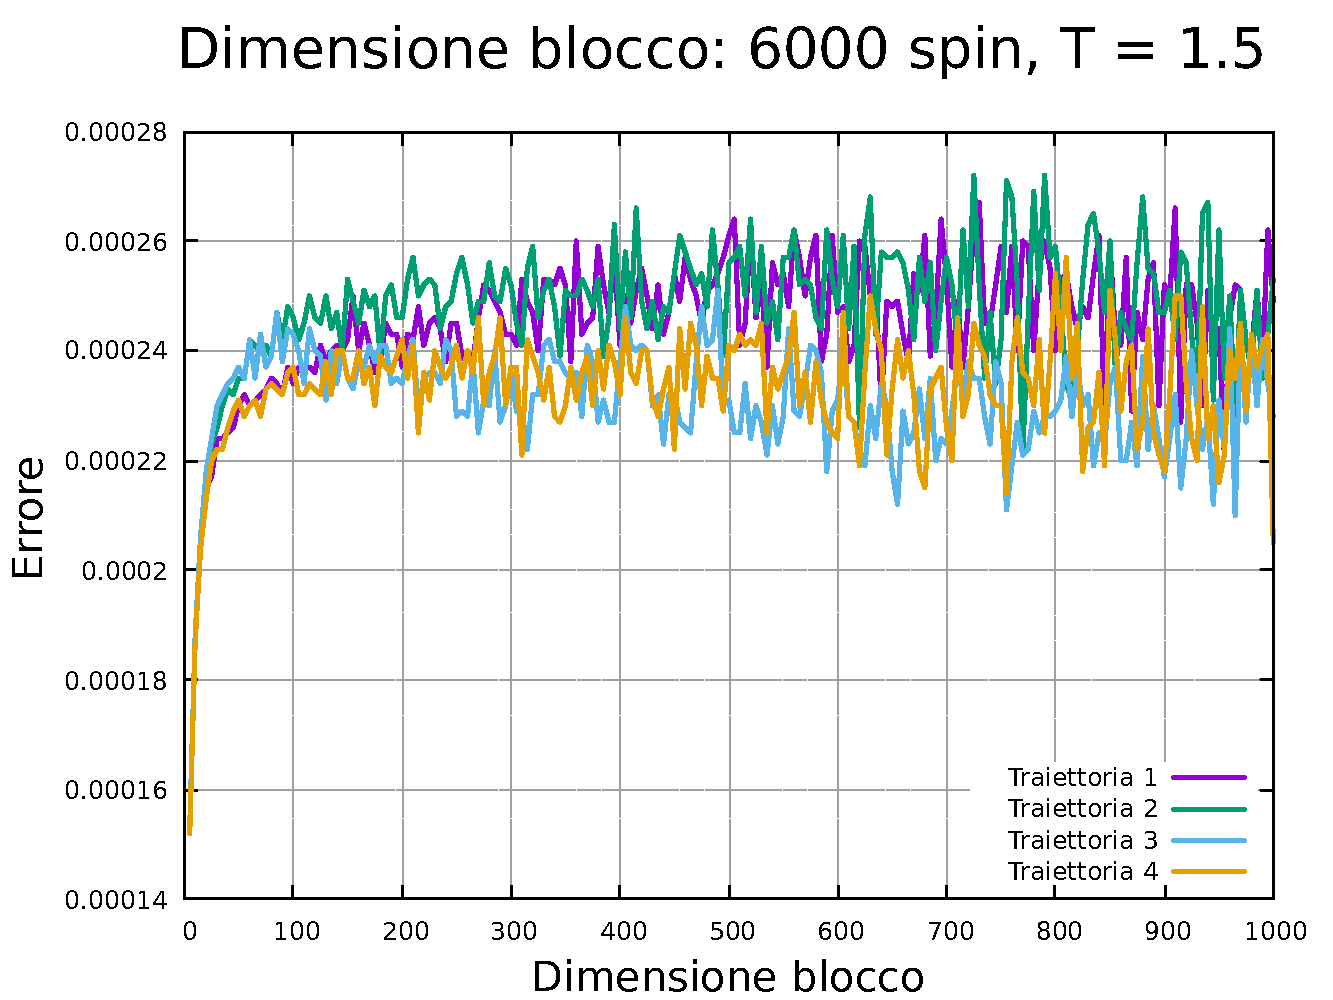
\includegraphics[page=1, width=\textwidth]{Immagini/simIsing1D/magn0.0/lblk/err_6000_1.5.pdf}
      \caption{$T\,=\,1.5$}
    \end{minipage}\hfill
    \begin{minipage}{0.45\textwidth}  
      \centering
      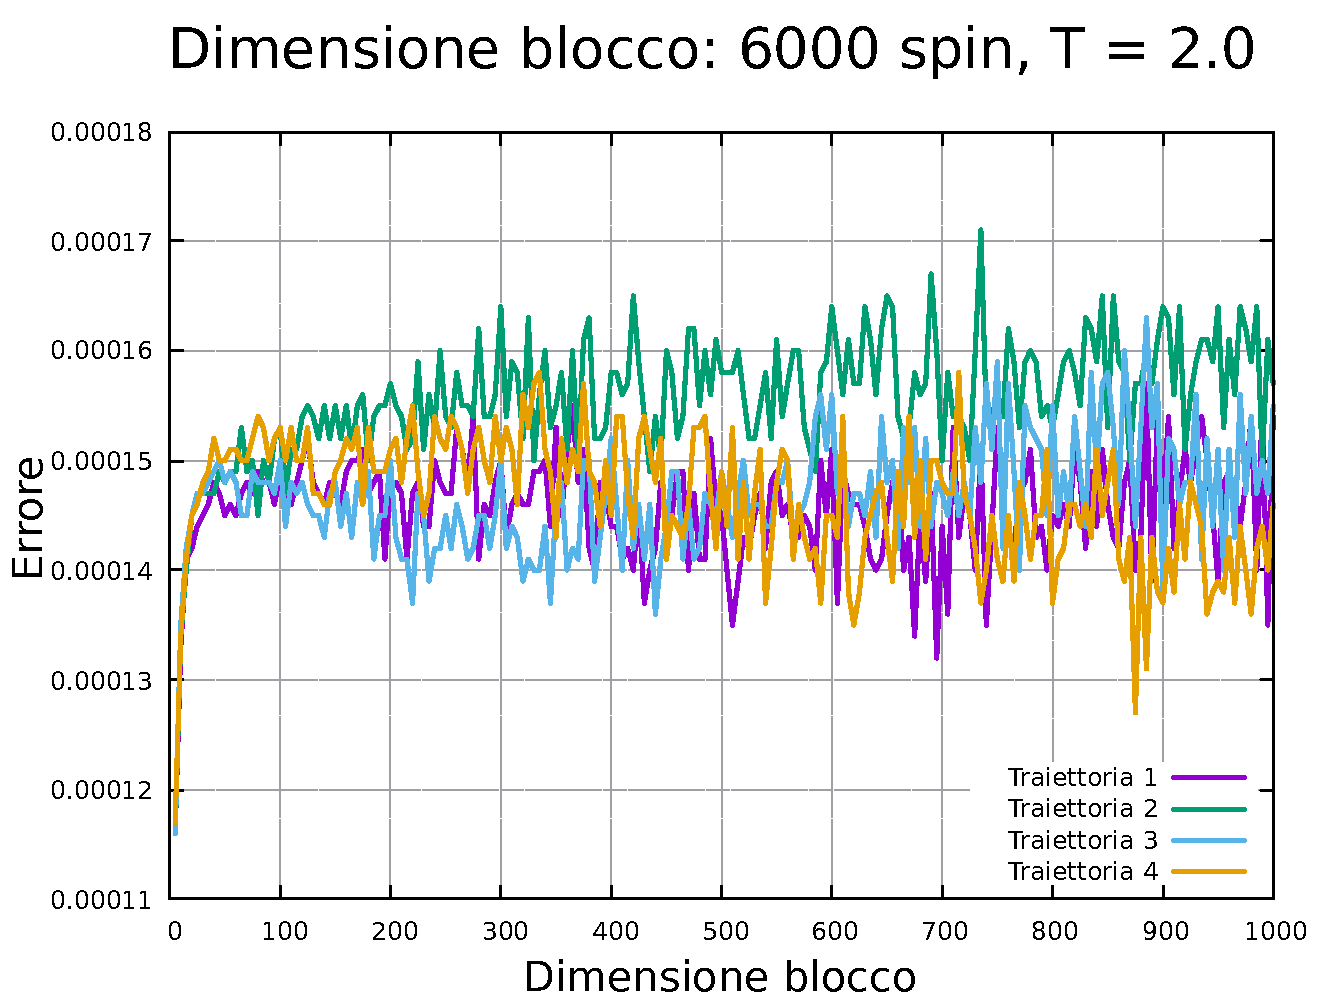
\includegraphics[page=1, width=\textwidth]{Immagini/simIsing1D/magn0.0/lblk/err_6000_2.0.pdf}
      \caption{$T\,=\,2.0$}
    \end{minipage}
    \caption{Errore in funzione della lunghezza dei blocchi per un modello di Ising 1D costituito da 6000 spin.}
\end{figure}

\vspace*{\fill}

\newpage

\vspace*{\fill}

\begin{figure}[htbp]
    \centering
    \begin{minipage}{0.45\textwidth}  
      \centering
      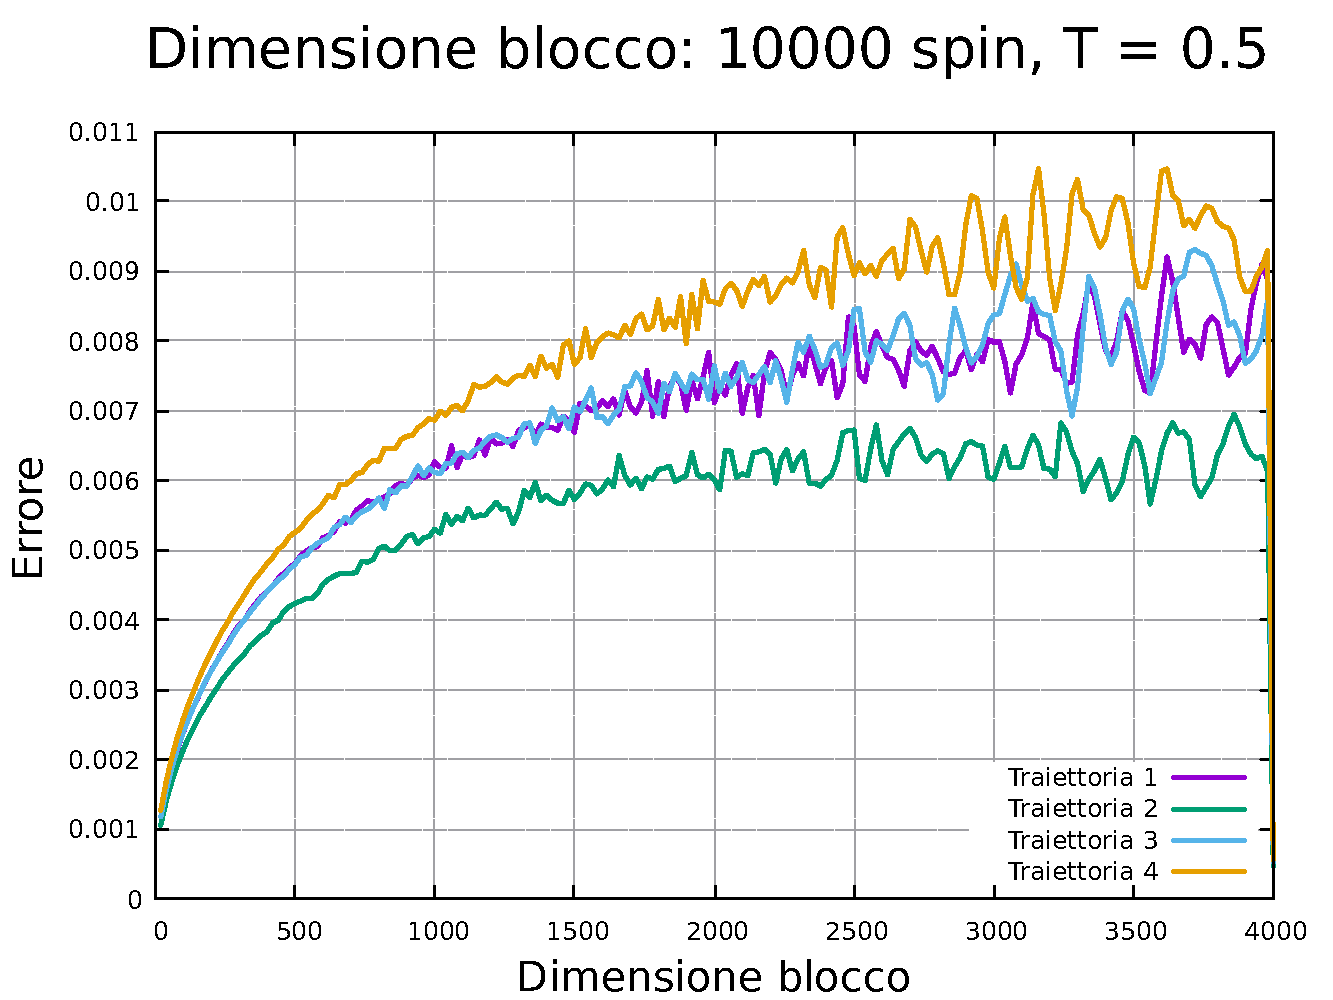
\includegraphics[page=1, width=\textwidth]{Immagini/simIsing1D/magn0.0/lblk/err_10000_0.5.pdf}
      \caption{$T\,=\,0.5$}
    \end{minipage}\hfill
    \begin{minipage}{0.45\textwidth}  
      \centering
      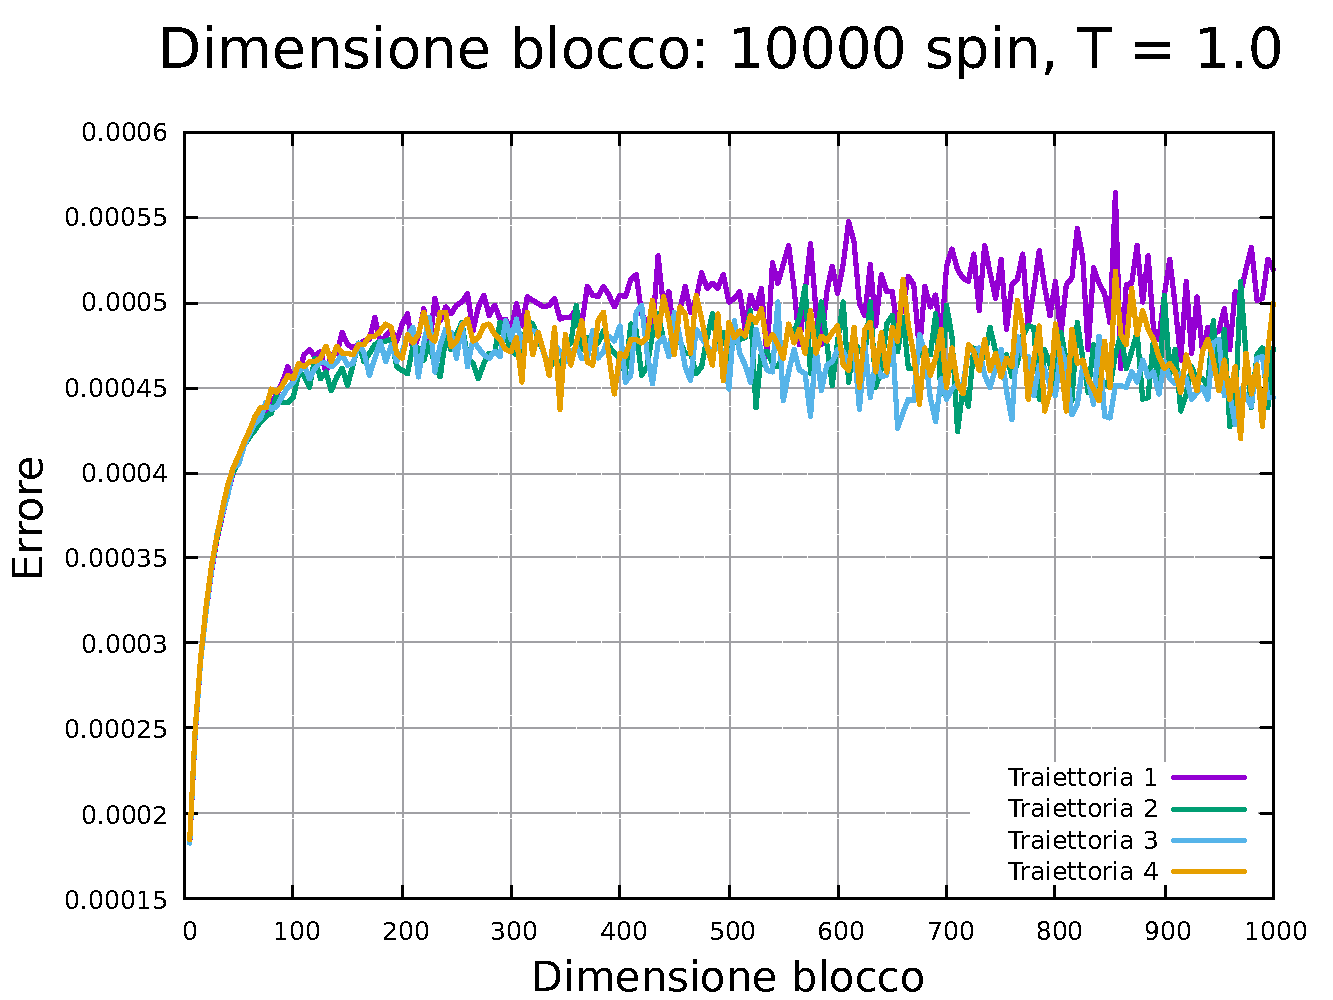
\includegraphics[page=1, width=\textwidth]{Immagini/simIsing1D/magn0.0/lblk/err_10000_1.0.pdf}
      \caption{$T\,=\,1.0$}
    \end{minipage}
    \vskip\baselineskip 
  
    \begin{minipage}{0.45\textwidth}  
      \centering
      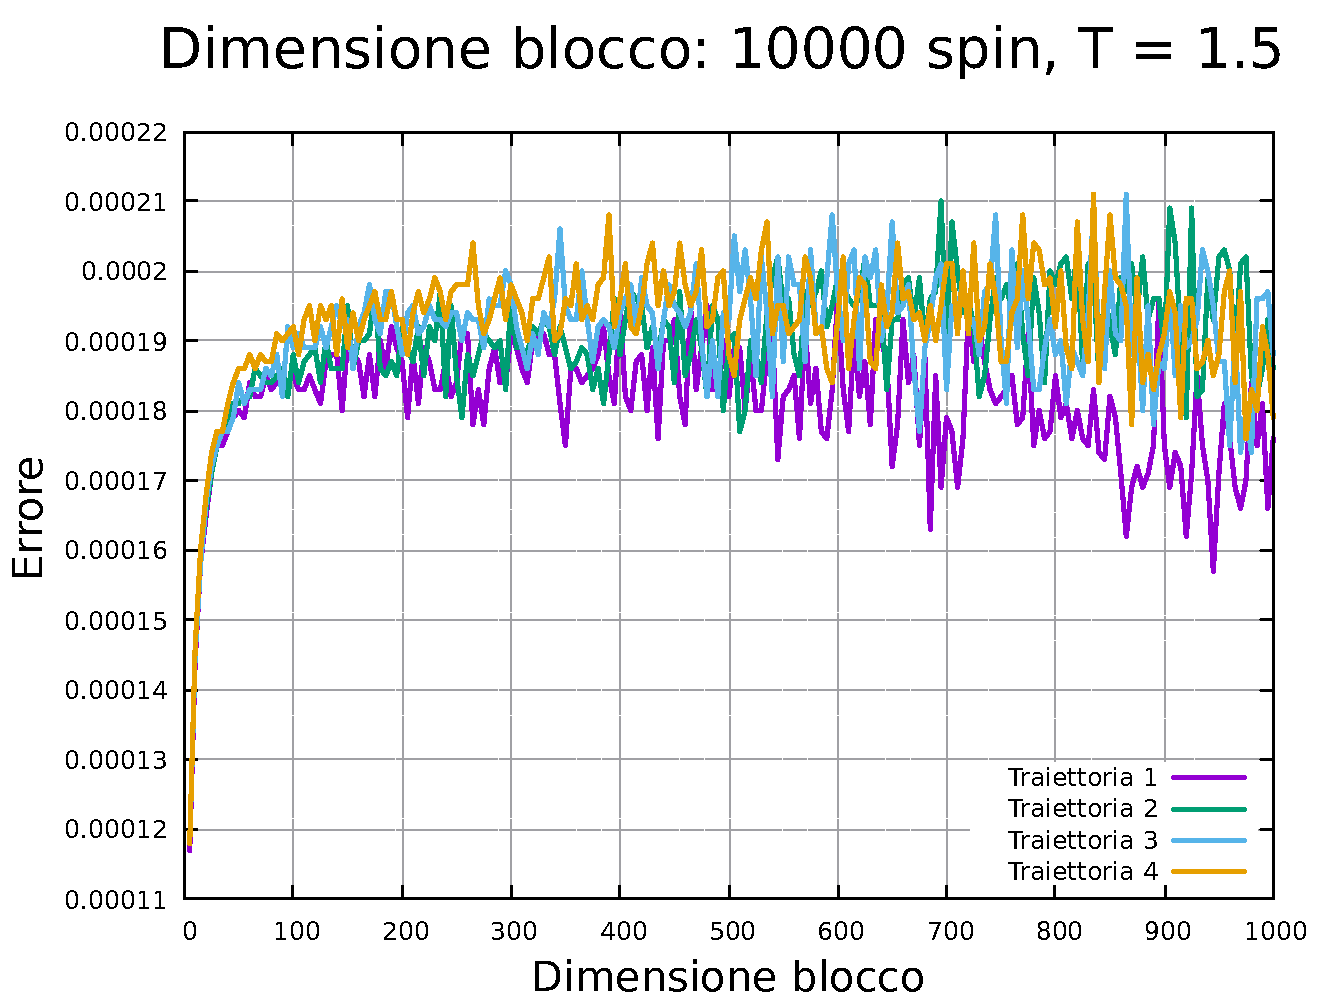
\includegraphics[page=1, width=\textwidth]{Immagini/simIsing1D/magn0.0/lblk/err_10000_1.5.pdf}
      \caption{$T\,=\,1.5$}
    \end{minipage}\hfill
    \begin{minipage}{0.45\textwidth}  
      \centering
      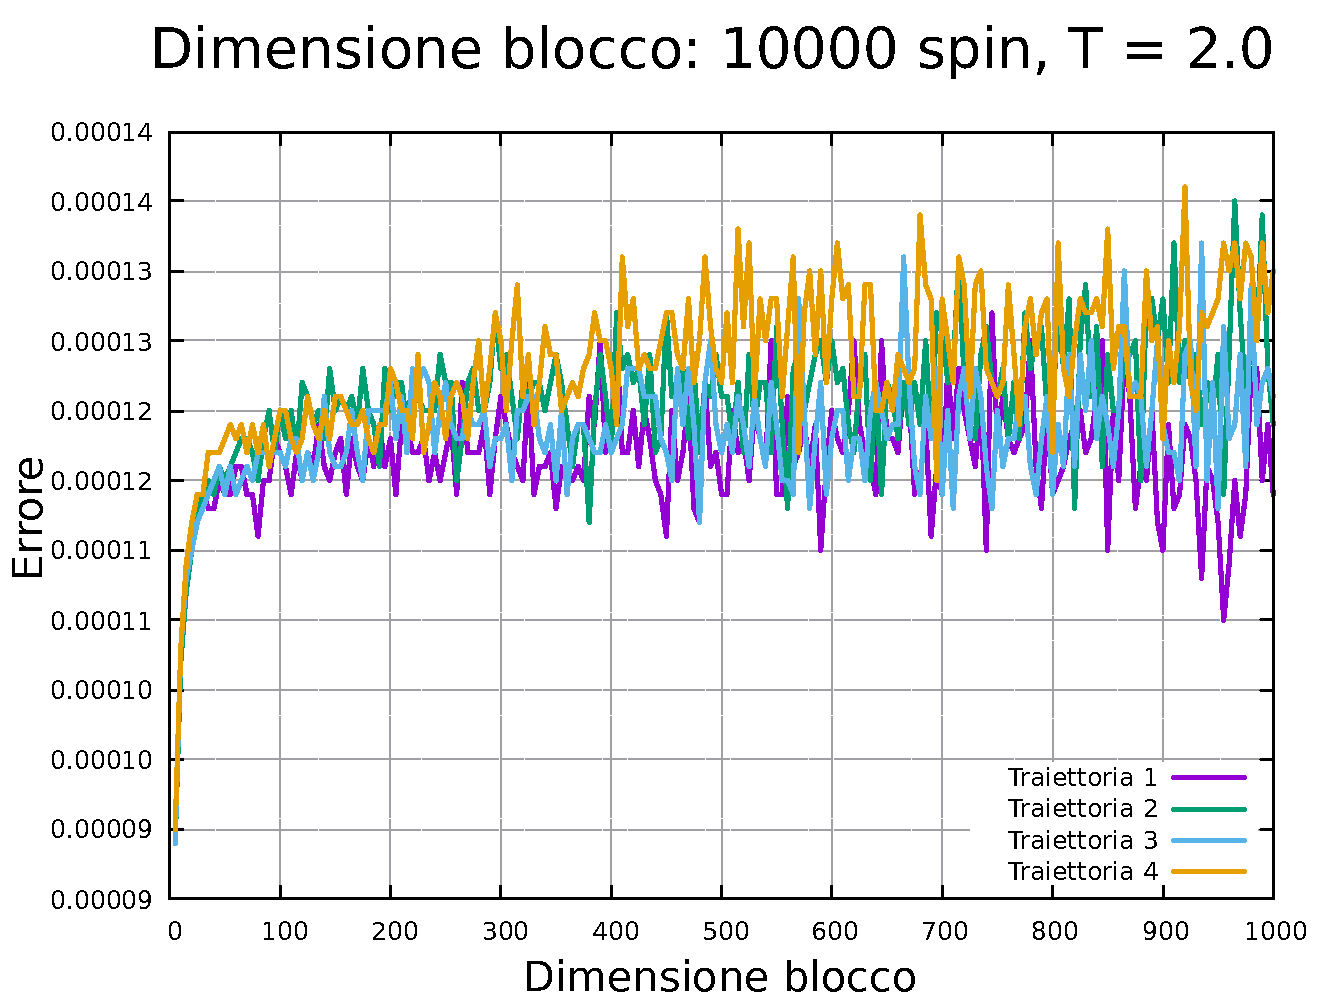
\includegraphics[page=1, width=\textwidth]{Immagini/simIsing1D/magn0.0/lblk/err_10000_2.0.pdf}
      \caption{$T\,=\,2.0$}
    \end{minipage}
    \caption{Errore in funzione della lunghezza dei blocchi per un modello di Ising 1D costituito da 10000 spin.}
\end{figure}

\vspace*{\fill}

\newpage



\subsection{Osservabili}

\vspace*{\fill}

\begin{figure}[htbp]
    \centering
    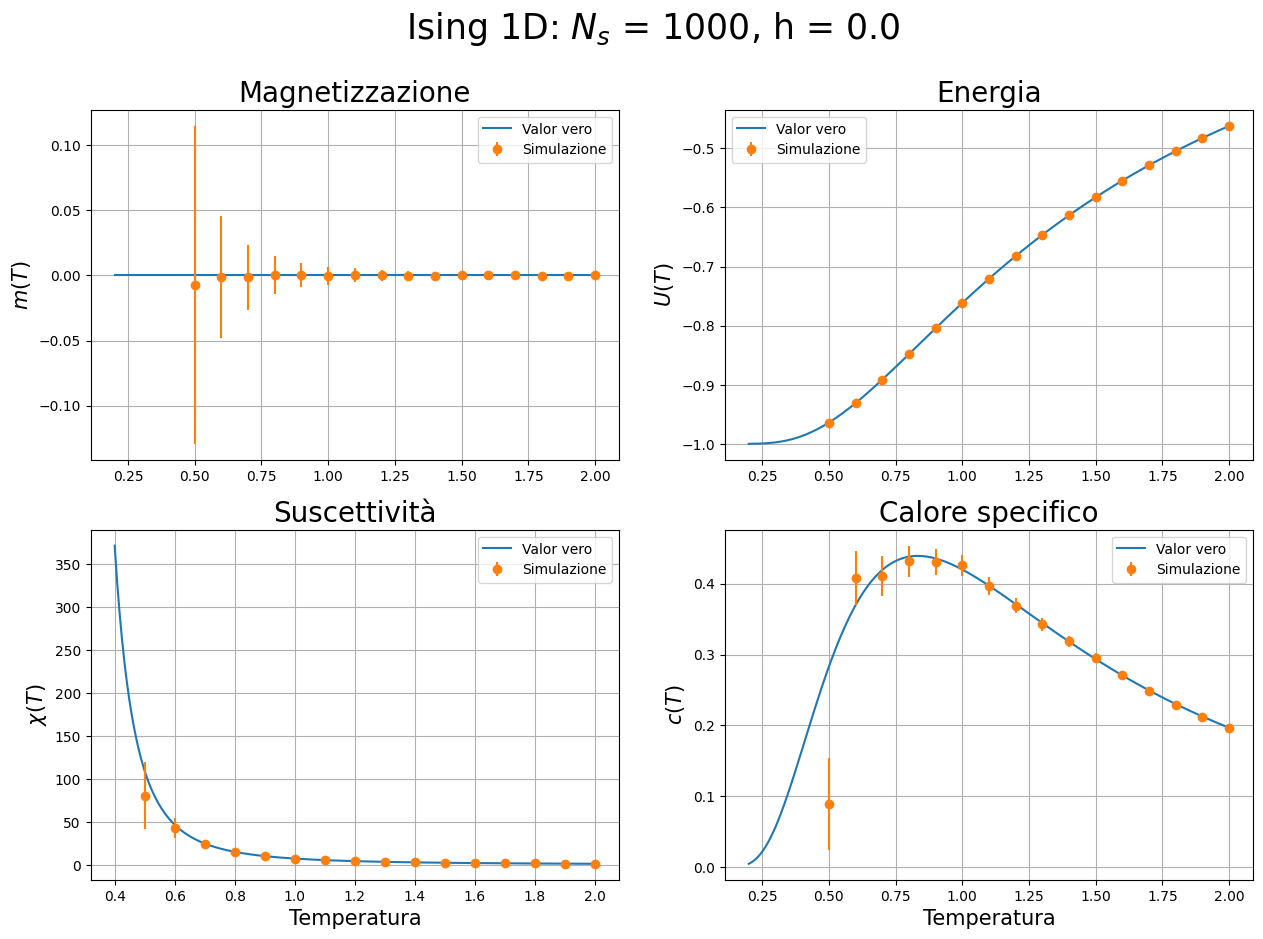
\includegraphics[page=1, width=\textwidth]{Immagini/simIsing1D/obs/obs_1000_0.0.png}
    \caption{Osservabili di un modello di Ising 1D costituito da 1000 spin al variare di T.}
\end{figure}

\vspace*{\fill}

\newpage

\vspace*{\fill}

\begin{figure}[htbp]
    \centering
    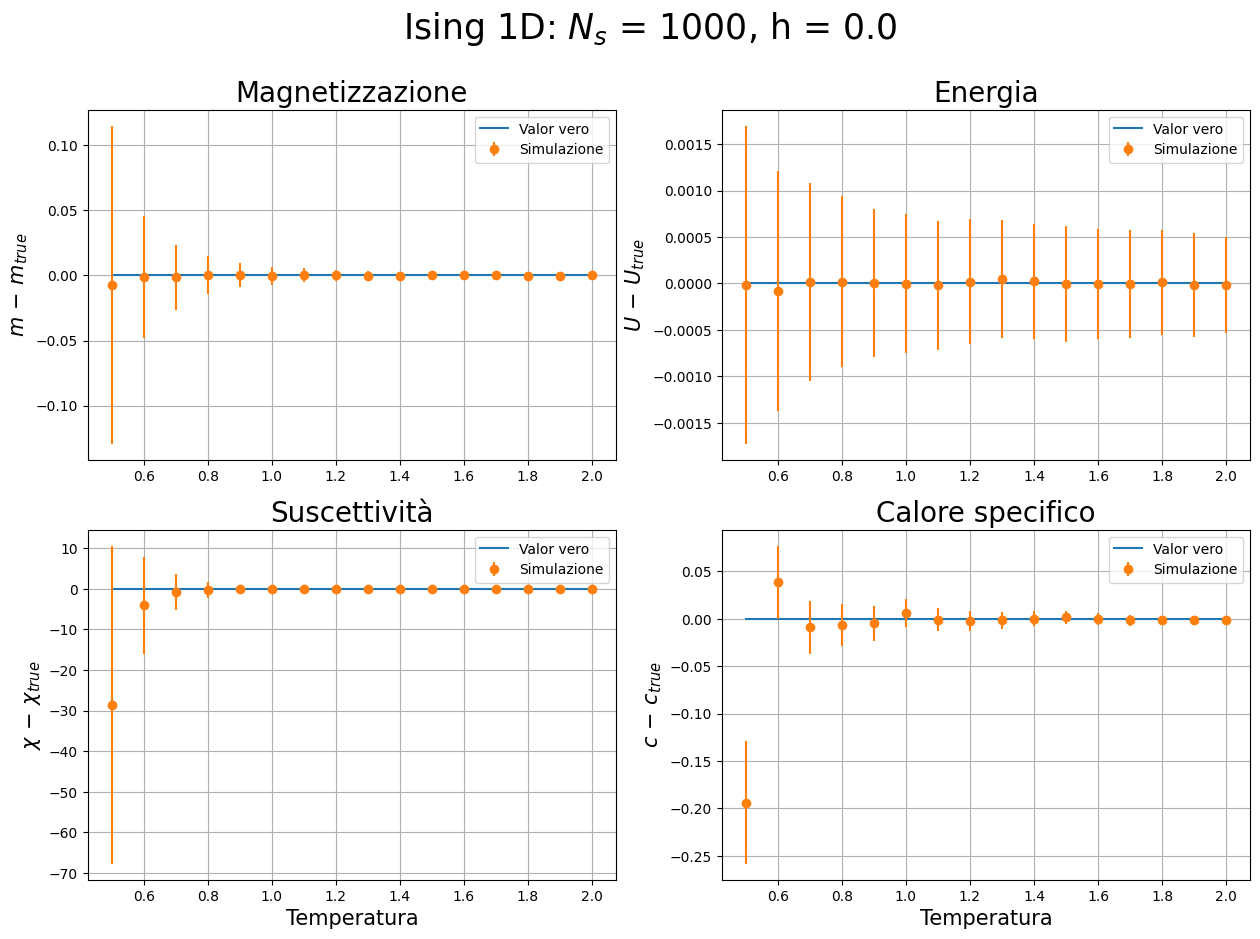
\includegraphics[page=1, width=\textwidth]{Immagini/simIsing1D/obs/obs_1000_0.0_diff.png}
    \caption{Differenza dal valor vero per un modello di Ising 1D costituito da 1000 spin al variare di T.}
\end{figure}

\vspace*{\fill}

\newpage

\vspace*{\fill}

\begin{figure}[htbp]
    \centering
    \includegraphics[page=1, width=\textwidth]{Immagini/simIsing1D/obs/obs_3000_0.0.png}
    \caption{Osservabili di un modello di Ising 1D costituito da 3000 spin al variare di T.}
\end{figure}

\vspace*{\fill}

\newpage

\vspace*{\fill}

\begin{figure}[htbp]
    \centering
    \includegraphics[page=1, width=\textwidth]{Immagini/simIsing1D/obs/obs_3000_0.0_diff.png}
    \caption{Differenza dal valor vero per un modello di Ising 1D costituito da 3000 spin al variare di T.}
\end{figure}

\vspace*{\fill}

\newpage

\vspace*{\fill}

\begin{figure}[htbp]
    \centering
    \includegraphics[page=1, width=\textwidth]{Immagini/simIsing1D/obs/obs_6000_0.0.png}
    \caption{Osservabili di un modello di Ising 1D costituito da 6000 spin al variare di T.}
\end{figure}

\vspace*{\fill}

\newpage

\vspace*{\fill}

\begin{figure}[htbp]
    \centering
    \includegraphics[page=1, width=\textwidth]{Immagini/simIsing1D/obs/obs_6000_0.0_diff.png}
    \caption{Differenza dal valor vero per un modello di Ising 1D costituito da 6000 spin al variare di T.}
\end{figure}

\vspace*{\fill}

\newpage

% \vspace*{\fill}
% 
% \begin{figure}[htbp]
%     \centering
%     \includegraphics[page=1, width=\textwidth]{Immagini/simIsing1D/obs/obs_10000_0.0.png}
%     \caption{Osservabili di un modello di Ising 1D costituito da 10000 spin al variare di T.}
% \end{figure}
% 
% \vspace*{\fill}
% 
% \newpage
% 
% \vspace*{\fill}
% 
% \begin{figure}[htbp]
%     \centering
%     \includegraphics[page=1, width=\textwidth]{Immagini/simIsing1D/obs/obs_10000_0.0_diff.png}
%     \caption{Differenza dal valor vero per un modello di Ising 1D costituito da 10000 spin al variare di T.}
% \end{figure}
% 
% \vspace*{\fill}
% 
% \newpage